\documentclass[12pt, a4paper, twoside, openright]{report}
%\documentclass[12pt, a4paper, twoside, openright]{article}		% 5p gir 2 kolonner pr side. 1p gir 1 kolonne pr side.
\usepackage[T1]{fontenc} 						% Vise norske tegn.
\usepackage[margin=2.5cm]{geometry}
%Options: Sonny, Lenny, Glenn, Conny, Rejne, Bjarne, Bjornstrup
%\usepackage[Bjornstrup]{fncychap}
\usepackage[grey]{quotchap}
% \usepackage[latin1]{inputenc}		% Velger tengsettet i dette dokumentet			
\usepackage[english]{babel}		
\usepackage[utf8]{inputenc}
\usepackage{lmodern}
\usepackage{graphicx}
\usepackage{tikz}
\usetikzlibrary{positioning}
\usepackage{hyperref}
\usepackage{amsmath,amssymb}
\usepackage{esint}
\usepackage[output-decimal-marker = {,}]{siunitx}
\usepackage[font=footnotesize,labelsep=period,labelfont=bf,margin=1cm]{caption}
\usepackage{import}
\usepackage{caption}
\usepackage{subcaption}
\usepackage{lipsum}
\usepackage{fixmath}
\usepackage[numbers]{natbib}
\usepackage[nottoc,numbib]{tocbibind}
\usepackage[toc,page]{appendix}
%\usepackage[raggedright]{titlesec}
%\usepackage{titlesec}
\usepackage{emptypage}
%\let\oldsection\section
%\def\section{\cleardoublepage\oldsection}
%\newcommand{\sectionbreak}{\clearpage}
%\usepackage{afterpage}
%\newcommand\blankpage{%
%    \null
%    \thispagestyle{empty}%
%    \addtocounter{page}{-1}%
%    \newpage}
\usepackage{fancyhdr}
\pagestyle{fancy}
\fancyhf{}
\fancyhead[EL]{\nouppercase\leftmark}
\fancyhead[OR]{\nouppercase\rightmark}
\fancyhead[ER,OL]{\thepage}

\setcounter{totalnumber}{5}
\renewcommand{\textfraction}{0.05}
\renewcommand{\topfraction}{0.95}
\renewcommand{\bottomfraction}{0.95}
\renewcommand{\floatpagefraction}{0.35}
\renewcommand{\d}[1]{\ensuremath{\operatorname{d}\!{#1}}}
\newcommand{\Imag}{{\Im\mathrm{m}}}   % Imaginary part 
\newcommand{\Real}{{\Re\mathrm{e}}}   % Real part
\DeclareRobustCommand{\orderof}{\ensuremath{\mathcal{O}}}
\setlength\parindent{24pt}
\numberwithin{equation}{chapter}
\numberwithin{figure}{chapter}
\numberwithin{table}{chapter}



\setcounter{totalnumber}{5}
\renewcommand{\textfraction}{0.05}
\renewcommand{\topfraction}{0.95}
\renewcommand{\bottomfraction}{0.95}
\renewcommand{\floatpagefraction}{0.35}

\makeatletter
\def\ps@pprintTitle{%
  \let\@oddhead\@empty
  \let\@evenhead\@empty
  \let\@oddfoot\@empty
  \let\@evenfoot\@oddfoot
}
\makeatother

\begin{document}

\begin{titlepage}

\newcommand{\HRule}{\rule{\linewidth}{0.5mm}} % Defines a new command for the horizontal lines, change thickness here

\center % Center everything on the page
 
%----------------------------------------------------------------------------------------
%	HEADING SECTIONS
%----------------------------------------------------------------------------------------

%\textsc{\LARGE Norwegian University of \\ \vspace{0.3cm} Science and Technology}\\[1.5cm] % Name of your university/college
\textsc{\Large Master thesis in applied physics and mathematics}\\[0.5cm] % Major heading such as course name
%\textsc{\large Minor Heading}\\[0.5cm] % Minor heading such as course title

%----------------------------------------------------------------------------------------
%	TITLE SECTION
%----------------------------------------------------------------------------------------

\HRule \\[0.4cm]
%{ \huge \bfseries The dynamics of skyrmions in an electric field}\\[0.4cm] % Title of your document
{ \huge \bfseries Electric control of skyrmion dynamics and spin torque oscillators in magnetic materials with Rashba spin-orbit coupling}\\[0.4cm]
\HRule \\[1.5cm]
 
%----------------------------------------------------------------------------------------
%	AUTHOR SECTION
%----------------------------------------------------------------------------------------

\begin{minipage}{0.4\textwidth}
\begin{flushleft} \large
\emph{Author:}\\
\O yvind \textsc{Johansen} % Your name
\end{flushleft}
\end{minipage}
~
\begin{minipage}{0.4\textwidth}
\begin{flushright} \large
\emph{Supervisor:} \\
Prof. Jacob \textsc{Linder} % Supervisor's Name
\end{flushright}
\end{minipage}\\[4cm]

% If you don't want a supervisor, uncomment the two lines below and remove the section above
%\Large \emph{Author:}\\
%John \textsc{Smith}\\[3cm] % Your name

%----------------------------------------------------------------------------------------
%	DATE SECTION
%----------------------------------------------------------------------------------------

{\large \today}\\[3cm] % Date, change the \today to a set date if you want to be precise

%----------------------------------------------------------------------------------------
%	LOGO SECTION
%----------------------------------------------------------------------------------------


\includegraphics[width=0.5\textwidth]{Figures/ntnu-logo.png} % Include a department/university logo - this will require the graphicx package
 
%----------------------------------------------------------------------------------------

\vfill % Fill the rest of the page with whitespace

\end{titlepage}
\cleardoublepage

%\title{Magnetization dynamics of domain walls and skyrmions in micromagnetics}
%\author{\O yvind Johansen}
%\date{\today}

%\maketitle
%\afterpage{\blankpage}
\pagenumbering{roman}

\chapter*{Abstract}
\addcontentsline{toc}{chapter}{Abstract}
\newpage

\chapter*{Sammendrag}
\addcontentsline{toc}{chapter}{Sammendrag}
\newpage

\chapter*{Preface}
\addcontentsline{toc}{chapter}{Preface}
%\\

\begin{minipage}{0.95\textwidth}
\begin{flushright}
\O yvind Johansen \\
Trondheim, Norway \\ 
June 2016
\end{flushright}
\end{minipage}\\[4cm]

\newpage

\tableofcontents

\newpage
%\afterpage{\blankpage}

\pagenumbering{arabic}

\chapter{Introduction}
% Magnetization dynamics in memory and logic devices
Most of the technological devices we use in our daily lives today are based on electronics, where we utilize the charge of the electron to transfer and process information. In recent decades an alternative to electronics has emerged, and its name is spintronics. Spintronic devices utilize the spin of the electron instead of its charge. These devices have several advantages over electronic devices, such as a lower power consumption and that the materials needed to realize the devices are fairly common metals \cite{Okamoto2014}, whereas electronic devices need rarer semiconductor materials to function. Spintronic devices are widely used in non-volatile memory applications, such as magnetoresistive random access memory (MRAM) \cite{Akerman2005,Katine2008}, racetrack memories \cite{Parkin2008} and spin-transfer torque magnetic random access memory (STT-MRAM) \cite{Kent2015}. Most of these applications are based on the giant magnetoresistance effect (GMR), which is that the resistance of a spin-polarized electrical current passing through a magnetic multilayer system is dependent on the orientation of the magnetic layers. When the magnetic moments of the different layers were anti-aligned the resistance of the current passing through the layers was much greater than the resistance of a current passing through magnetic layers with aligned magnetic moments. The discovery of this effect by Fert \cite{Fert1988} and Gr\"{u}nberg \cite{Grunberg1989} in 1988 was awarded by the Nobel prize in physics in 2007. This effect makes it possible to use magnetic multilayers for information storage in the form of bits, as we have a high-resistance and a low-resistance state, which can be assigned to the values zero and one. In addition, this information is not necessarily lost in the absence of an applied electric current or magnetic field, as the magnetic layers can keep their orientation in an equilibrium state. This makes the spintronic devices particularly interesting for non-volatile memory applications.

Being able store information in magnetic systems is not too interesting by itself, we also need to be able to read and write the information effectively. This is where magnetization dynamics comes into play, a topic that this thesis will mainly revolve around. While it is known that magnetic moments can be manipulated by magnetic fields, this method is often impractical for nano-scale devices due to the large fields required to manipulate the magnetic moments in a very localized region. It has been discovered, however, that the magnetization in a magnetic material can also be manipulated by electrical means. An experiment by Johnson and Silsbee in 1985 showed that the spin direction of the electrons in a current passing through a magnetic layer was aligned with the magnetic moment in the layer \cite{JohnsonSilsbee1985}. The magnetization in the film must therefore have exerted a torque on the spins of the conduction electrons. It is then reasonable to think that the spins of the conduction electrons will also exert a torque on the magnetization in the magnetic layer. This was shown theoretically by Berger \cite{Berger1978,Berger1984,Berger1992,Berger1996} and Sloncewski \cite{Slonczewski1996}, and later observed experimentally \cite{Tsoi1998}. This torque, known as the spin-transfer torque, could be used to switch the magnetization direction of one of the magnetic layers in a multilayer system \cite{Myers1999,Sun1999,Katine2000}. It is therefore a very useful mechanism in writing techniques in spintronic devices. 

% The use of skyrmions vs domain walls (critical current, Joule heating, storage density)
Spin-transfer torques have also been shown to induce a translational motion of magnetic textures, such as domain wall motion \cite{Gan2000,Vernier2004}. This is very useful in information processing, as we can move the information encoded in magnetic domains without any motion of physical components. This is utilized in racetrack memories \cite{Parkin2008}. This motion of magnetic textures is not without problems, however. Ideally we would move these magnetic textures in a pure translational manner, but above some critical current strength the motion of magnetic domain walls has been shown to undergo a Walker breakdown \cite{SchryerWalker1974}. This Walker breakdown is an excitation of a different type of dynamics of the domain wall, in the form of rotational motion. In addition, at the current density needed to move domain walls Joule heating becomes a concern \cite{Yamaguchi2005}, causing energy loss to heat generation and thermal effects in the domain wall motion. Another magnetic texture known as the magnetic skyrmion has been of considerable interest lately, however. This is due to the fact that the critical current necessary to move them has been shown to be as low as $10^6$ A/m$^2$ \cite{Jonietz2010,Schulz2012,Yu2012}, whereas domain walls have a critical current in the range $10^{10}-10^{12}$ A/m$^2$ \cite{Grollier2003,Parkin2008}. This makes it possible to move them without considerable effects from Joule heating. In multiferroic materials it is even possible to create skyrmion based memory devices without any Joule heating effects at all \cite{Mochizuki2015}, as they can there be controlled by electric fields. The dynamics of skyrmions has also been shown to be controllable by electric fields even in ferromagnetic materials \cite{Upadhyaya2015}.  Skyrmions are topologically stable objects, meaning  they are also suitable for non-volatile memory applications. They are also of particular interest due to their ability for an extremely dense storage of information \cite{Fert2013}, as a single skyrmion can span just a few nanometers. In addition, methods that would make it possible to nucleate skyrmions by injection of a spin-polarized current \cite{Sampaio2013}, spin-waves \cite{Liu2015} or by applying mechanical stress \cite{Nii2015} have been suggested. This ability to manipulate skyrmions makes them very attractive in memory applications. The downside of skyrmions with respect to magnetic domain walls is that the skyrmion velocities obtained so far are well below what is achievable with magnetic domain walls \cite{Fert2013,Yang2015}. 

% Applications of spin torque oscillators
A third use of the spin-transfer torque, in addition to magnetization switching and translation of magnetic textures, is the precession of magnetic moments it can induce in magnetic multilayer systems \cite{Tsoi2000,Kiselev2003,Rippard2004}. When the magnetic moments in a multilayer system precess with respect to one another, so the projection of one magnetic moment onto another varies in time, this will cause an oscillation in the resistance of a current passing through the system due to the giant magnetoresistance effect. A direct current passing through the multilayer system will then be transformed into an alternating current. Such a system with a self-sustained precession in the magnetic layers is known as a spin-torque oscillator \cite{Silva2008,Kim2012STO}. These oscillators are able to generate a wide range of frequencies in the output signal, spanning the range of 100s of MHz to 100s of GHz \cite{Katine2008,Silva2008,Sun2008}. In addition, the frequency obtained can easily be tuned by the strength of the applied current. This type of self-sustained precession has been shown to occur in both ferromagnetically \cite{Zhou2013} and antiferromagnetically \cite{Klein2012} coupled magnetic layers, although Ref. \cite{Zhou2013} was unable to reproduce the results of Ref. \cite{Klein2012}. 

% Interest in RSOC and its applications
Both skyrmions and spin-torque oscillators appear in systems with a broken inversion symmetry. Skyrmions appear in chiral magnets, while spin-torque oscillators are based magnetic multilayer systems, which have a broken inversion symmetry at the interfaces of the different layers. When we have a system with broken inversion symmetry a current passing perpendicular to the direction of the asymmetry will induce a spin-orbit coupling in the system, known as Rashba spin-orbit coupling \cite{BychovRashba1984,Heide2006}. This type of spin-orbit coupling has proven to cause interesting effects in many different areas \cite{Manchon2015}, such as the appearance of an intrinsic spin Hall effect \cite{Sinova2004}. The spin-orbit coupling was also an important mechanism in the implementation of the spin field-effect transistor by Datta and Das \cite{DattaDas1990}. One of the advantages of Rashba spin-orbit coupling is its ability to be modified by the application of an electric field via gate voltages \cite{Schultz1996,Nitta1997}. This way the strength of the inversion asymmetry can be controlled to some extent. A discovery that is of particular interest to us is that Rashba spin-orbit coupling can also contribute to magnetization switching and self-sustained oscillations in spin-torque oscillators \cite{Miron2011,Duan2014}.

% General structure of thesis
In this thesis we will study the magnetization dynamics of a single skyrmion (which is driven by spin-transfer torques and inhomogenous electric fields) and spin-torque oscillators, both in the presence of Rashba spin-orbit coupling. We first introduce the micromagnetic model and the Landau--Lifshitz--Gilbert equation as a foundation for our calculations. Before deriving the equations of motion of the skyrmion from the Thiele equation, we briefly discuss the structure, symmetries and dynamical properties of the skyrmion. The analytical solution of the Thiele equation is then compared to a full numerical solution of the Landau--Lifshitz--Gilbert equation. Lastly, we combine analytical and numerical calculations to find the spin-torque oscillator state and its frequency spectrum based on the Landau--Lifshitz--Gilbert--Slonczewski equation. 

\chapter{The micromagnetic model}
In this thesis we will base our work on the micromagnetic model. This model is a semi-classical theory that is conventionally used to describe both the equilibrium and dynamics of the magnetization in a material on a nanometer to micrometer length scale. This length scale is large enough to assume a continuum approximation, we can consider the magnetization as a smooth and continuously varying vector field in space, as it is greater than the typical atomic length scale. On this length scale it is also not necessary to do a full quantum mechanical treatment of the system, making it justifiable to primarily treat quantities as expectation values instead of operators. The length scale is small enough, however, to be able to successfully describe patterns in the magnetization that are observed in nature, such as magnetic domain walls or magnetic skyrmions. This model is also able to describe the motion of such magnetization patterns well, which makes it a highly attractive model in the field of magnetization dynamics.
%\section{Zeeman energy}
%The Zeeman energy is the energy contribution from the interaction between the magnetization $\mathbold{M}(\mathbold{r})$ in the magnetic material and an external magnetic field $\mathbold{H}_Z(\mathbold{r})$. This energy can be expressed as
%\begin{align}
%E_Z = -\mu_0\int \d V \mathbold{M}(\mathbold{r})\cdot\mathbf{H}_Z(\mathbold{r}),
%\end{align}
%with $\mu_0$ being the vacuum permeability.
\section{Energy terms in micromagnetics}
In conventional micromagnetics there are five contributions to the micromagnetic energy. These are the exchange energy, the anisotropic energy, the Zeeman energy, the demagnetization energy, and the magneto-elastic energy. Of these five energies we will only discuss the former three. The demagnetization energy is not considered as it is mainly dominant over larger length scales, and the length scale that we will primarily consider is on the nanometer length scale. The magneto-elastic energy is also neglected, as we will not consider elastic distortion of the lattice. We will, however, also consider energy contributions that are not included in conventional micromagnetics. We will treat these energy contributions in the same manner, assuming a continuum model of the magnetization.
\subsection{Exchange energy} \label{sec:Exchange}
Ferromagnetism occurs in materials where the spins tend to align with each other, and thereby being able to generate an observable magnetic field outside of the material. The mechanism behind this is the exchange interaction between the spins. In ferromagnetic materials the system can lower its energy by having parallel neighboring spins. This is described by the Heisenberg Hamiltonian,
\begin{align}
H = - J\sum_{\langle i,j\rangle} \mathbold{S}_i\cdot\mathbold{S}_j,
\end{align}
with $J$ being the exchange integral which is positive for ferromagnetic materials and $\mathbold{S}$ a dimensionless spin-vector. The spins can be expressed in terms of the magnetization, which is the average magnetic moment. As the magnetic moment and the spin of an electron are anti-parallel, this relation becomes
\begin{align}
\label{eq:ExchangeHamiltonian}
\mathbold{S}_i = -\frac{S}{M_s}\mathbold{M}_i,
\end{align}
with $M_s$ being the saturation magnetization and $S$ the magnitude of the spin. The magnetization is a classical vector, and in micromagnetism it is treated as a slowly varying smooth function. One can therefore perform a Taylor expansion of it. By doing that, one can show \cite{Project} that the energy density can be written as
\begin{align}
\epsilon_{EX} = \frac{\textrm{d} E_{EX}}{\textrm{d} V} = -\frac{A}{M_s^2}\mathbold{M}(\mathbold{r})\mathbold{\nabla}^2\mathbold{M}(\mathbold{r}) = \frac{A}{M_s^2}\partial_i\mathbold{M}(\mathbold{r})\partial_i\mathbold{M}(\mathbold{r}), \label{eq:exchDensity}
\end{align}
with $A$ being the exchange stiffness
\begin{align}
A = \frac{J S^2}{2a}
\end{align}
and $a$ being the lattice constant.

\subsection{Zeeman energy}
When turning on an external magnetic field in a magnetic material, the magnetic moments in the material tend to align with the magnetic field. This is due to the Zeeman interaction, which will go to a lower energy state if the magnetic moments and external field are aligned. The Zeeman interaction energy density is given by
\begin{align}
\epsilon_Z = -\mu_0 \mathbold{M}\cdot\mathbold{H}_Z,
\end{align}
with $\mathbold{H}_Z$ being the external magnetic field.

\subsection{Perpendicular magnetic anisotropy} \label{sec:PMA}
In some magnetic materials we may have something known as magnetic anisotropy. As the name indicates, there is an anisotropy in the material that makes certain magnetization directions more energetically favorable than others. This mostly stems from the spin-orbit coupling. If one considers the rest frame of the electron instead of the proton, the proton is orbiting the electron and thereby causing a temporal varying electric field. Amp\`{e}re's circuital law then says that the electron observes a magnetic field proportional to the orbital motion of the proton. This magnetic field then interacts with the magnetic moment (proportional to the spin) of the electron like in the Zeeman interaction, except here due to internal fields, hence the name spin-orbit coupling. Taking this into consideration as well as the atomic structure in the material, one can see that one could end up with a material where the magnetic field the electrons experience from the spin-orbit coupling would allow one direction to be easier magnetized than others.

In some layered ultrathin film structures, such as Pd/Co \cite{Carcia1985}, it has been discovered that the magnetization has a lower energy when it is perpendicular to the films. This means that the easy axis of the material is perpendicular to the films, and we then have something called perpendicular magnetic anisotropy (PMA). The anisotropic energy is independent of the direction the magnetization has along the easy axis, meaning the energy is the same if the magnetization points into or out of the films. Letting $K$ be the anisotropy constant and $\theta$ the angle to the normal of the films, the anisotropic energy density can then be written as
\begin{align}
\epsilon_{PMA} = K\sin^2\theta \label{eq:PMADensity}
\end{align} 
to the lowest order in $\theta$. Here we have normalized the energy density in such a way that if the magnetization points along the easy axis the energy density is zero.

\subsection{Voltage induced magnetic anisotropy} \label{sec:VIMA}
One form of perpendicular magnetic anisotropy occurs at the interface between certain materials. This has been attributed to the exchange interaction between $p-$ and $d-$oribitals at material interfaces, such as the 3$d$ orbital in Fe and 2$p$ orbital in O at an Fe/MgO interface \cite{Matsukura2015}. As this is a magnetic anisotropy that only occurs at the surface of the material, it will only be of importance in ultra-thin magnetic films where surface effects are of a greater importance. It has also been discovered that one can modify the strength of this surface magnetic anisotropy with an external electric field. The reason for the change of strength in the magnetic anisotropy is the modification of the occupation number in the 3$d$ orbitals in Fe, thereby affecting the $p$-$d$ exchange interaction that is the origin of the magnetic surface anisotropy \cite{Maruyama2009}. It was found that in a thin-film system with an Fe/MgO interface where the Fe layer consisted of only a few monoatomic layers a change of approximately 40\% could be achieved in the magnetic surface anisotropy by application of an external electric field. As it is relatively easy to generate a localized electric field, one can therefore create an energy landscape to influence the dynamics of magnetization patterns. An example of this was shown by Upadhyaya et al. by guiding dipole-dipole interaction skyrmions with voltage gates \cite{Upadhyaya2015}.

As the voltage induced magnetic anisotropy behaves as PMA, the energy density must then have the same form as that of $\epsilon_{PMA}$ in \eqref{eq:PMADensity} and be dependent on the electric field. If one assumes that the modification of the electric field on the PMA is linear in the electric field, the energy density can be written as
\begin{align}
\epsilon_{EF} = \eta E(\mathbold{r}) \sin^2\theta,
\end{align}
where $\eta$ is a materialistic constant describing the strength of the modification of PMA by the electric field, and the electric field strength $E(\mathbold{r})$ is the $z$-component of the electric field as a function of position in the thin film. 

\subsection{Ruderman--Kittel--Kasuya--Yosida interaction}
In metals, there is also another type of exchange interaction between magnetic moments in addition to the one described in Section \ref{sec:Exchange}. This interaction between nuclear magnetic moments is an indirect interaction. First a conduction electron in the atom interacts with the nuclear magnetic moment (proportional to its spin) through the hyperfine interaction. The hyperfine interaction is similar to the spin-orbit coupling discussed in Section \ref{sec:PMA}. Instead of being in the rest frame of the electron, however, we consider the magnetic field seen in the rest frame of the nucleus due to the orbital motion of the electron. In addition, as the electron carries with it an intrinsic magnetic moment, it will generate a magnetic field that will interact with the spin of the nucleus. In short, the hyperfine interaction consists of spin-orbit and spin-spin interactions seen from the rest frame of the nucleus. Going back to the conduction electron that has interacted with the nuclear magnetic moment through the hyperfine interaction, it can also interact with another nuclear magnetic moment after interacting with the first. It can therefore act as a mediating particle for the interaction between the magnetic moments of two different nuclei. This interaction is known as the Ruderman--Kittel--Kasuya--Yosida (RKKY) interaction \cite{RudermanKittel1954, Kasuya1956, Yosida1957, Vleck1962}, and its Hamiltonian is given by
\begin{align}
    \label{eq:RKKYHamiltonian_old}
    H_{\text{RKKY}} = \frac{\mathbold{I}_i\cdot\mathbold{I}_j}{4}\frac{|\Delta k_m k_m|^2m^*}{(2\pi)^3 R_{ij}^4 \hbar^2} \left[2k_mR_{ij}\cos\left(2k_mR_{ij}\right) - \sin \left(2k_mR_{ij}\right)\right].
\end{align}
Here $\mathbold{I}_i$ and $\mathbold{I}_j$ are the nuclear magnetic moments, $R_{ij}$ the distance between the magnetic moments, $k_m$ the wave number of the conduction electrons, $m^*$ the effective mass of the electrons and $\Delta k_m k_m$ is a factor describing the strength of the hyperfine interaction. What is important to note here is that the RKKY Hamiltonian acts similarly to the exchange Hamiltonian \eqref{eq:ExchangeHamiltonian} in a manner that it is a symmetric interaction between spins, and that the coupling strength between the spins is a function of distance. Moreover, unlike the exchange interaction, this function of distance can either be positive or negative depending on the value of $k_mR_{ij}$. This means that we can alter if two magnetic moments are ferromagnetically or antiferromagnetically coupled to each other by increasing or decreasing the distance between them. The way the interaction is formulated in \eqref{eq:RKKYHamiltonian_old} it is between two nuclear magnetic moments. However, the RKKY  interaction can also occur in a multilayer system such as F$_1$/N/F$_2$ where F$_i$ are thin uniformly magnetized magnetic metals and N is a non-magnetic metallic spacer, as shown by Parkin and Mauri in \cite{Parkin1991}. If one lets the magnetization in F$_i$ be $\mathbold{M}_i$, the RKKY interaction energy in F$_i$ can then be written as
\begin{align}
    H_{\text{RKKY}} = -\frac{J_{\text{RKKY}}(R_{ij})}{d_iM_s^2}\mathbold{M}_i\cdot\mathbold{M}_j,
\end{align}
with $J_{\text{RKKY}}(R_{ij})$ being the distance dependent coupling strength between the magnetic moments that can be both positive and negative, and $d_i$ being the thickness of F$_i$. The magnetic layers will then have a ferromagnetic coupling when $J_{\text{RKKY}}>0$ and an antiferromagnetic coupling when $J_{\text{RKKY}}<0$.

\subsection{The Rashba effect}
In materials where the motion of the electrons is confined to a plane, and the inversion symmetry is broken along the axis perpendicular to that plane, there is a splitting of the spin energy levels. Inversion symmetry can for example be broken at the interface between two materials \cite{Heide2006}. The inversion asymmetry causes an electric field perpendicular to the plane of motion, as the gradient of the electrostatic potential becomes non-zero when inversion symmetry is broken ($V(\mathbold{r}) \neq V(-\mathbold{r})$). When particles move in an electric field, they experience a magnetic field which can be seen by performing a Lorentz transformation into the particles' restframe. This magnetic field is proportional to $\mathbold{v}\times\mathbold{E}$. Because of the magnetic field the energy levels become spin dependent, as the field couples to the spin. This is described by the Rashba Hamiltonian \citep{BychovRashba1984}
\begin{align}
H_R &= \frac{\alpha_R}{\hbar}\mathbold{\sigma}\cdot(\mathbold{p}\times\mathbold{\hat{n}}) = \alpha_R (\mathbold{\sigma}\times\mathbold{k})\cdot\mathbold{\hat{n}}.
\label{eq:RashbaH}
\end{align}
Here $\alpha_R$ is the Rashba parameter, $\mathbold{p} = \hbar\mathbold{k}$ the momentum of the electrons, $\mathbold{\hat{n}}$ a unit vector perpendicular to the plane of motion (along the direction of broken inversion symmetry) and $\mathbold{\sigma}$ is a vector of the Pauli matrices. This can be seen as the magnetic field points along the direction $\mathbold{v}\times\mathbold{E}$, and as $\mathbold{p}\propto\mathbold{v}$ and $\mathbold{E}$ points along the direction of broken inversion symmetry given by $\mathbold{\hat{n}}$, the magnetic field therefore points along $\mathbold{p}\times\mathbold{\hat{n}}$. According to the Zeeman energy the energy should be then proportional to $\mathbold{\sigma}\cdot(\mathbold{p}\times\mathbold{\hat{n}})$, and this proportionality constant is given by $\alpha_R$, the value of which contains the physics of the broken inversion symmetry. This effect is a form of spin-orbit interaction, as the spin of the electron ($\propto \mathbold{\sigma}$) interacts with its own motion ($\mathbold{v}$). This effect is therefore also called Rashba spin-orbit coupling (RSOC).

\subsection{The Dzyaloshinskii--Moriya interaction}
The Dzyaloshinskii--Moriya interaction (DMI) is an antisymmetric exchange coupling between spins, given by the Hamiltonian
\begin{align}
H_{DM} = \sum_{\langle i,j\rangle}\mathbold{D}_{ij}\cdot(\mathbold{S}_i\times\mathbold{S}_j). \label{eq:DMIHamiltonian}
\end{align}
This interaction only occurs in materials where the inversion symmetry is broken. The magnitude of $\mathbold{D}_{ij}$ depends on the material properties, and the direction of $\mathbold{D}_{ij}$ depends on the symmetry of the atomic structure in the material. Moriya showed \cite{Moriya1960} that if there is an $n$-fold axis (with $n \geq 2$) along the axis between the particles with spins $\mathbold{S}_i$ and $\mathbold{S}_j$, $\mathbold{D}_{ij}$ will be parallel to that axis. Using that in a Taylor expansion of \eqref{eq:DMIHamiltonian}, it can be shown \cite{Project} that the energy density becomes
\begin{align}
\label{eq:DMBulk}
\epsilon_{DM}^{\textrm{(bulk)}} = \frac{D}{M_s^2}\mathbold{M}\cdot(\mathbold{\nabla}\times\mathbold{M}).
\end{align}
On the other hand, if there is a mirror plane located at the center of the line between the particles with spins $\mathbold{S}_i$ and $\mathbold{S}_j$ that is perpendicular to the axis intersecting them, the vector $\mathbold{D}_{ij}$ lies in the mirror plane. In a more specific case where the interaction between the spins $\mathbold{S}_i$ and $\mathbold{S}_j$ is mediated by a third magnetic particle (different from the other two) located in the mirror plane, $\mathbold{D}_{ij}$ is perpendicular to the triangle spanned by the three particles as illustrated in Figure \ref{fig:InterfacialDMI}. 
%\begin{figure}[h!]
%\begin{center}
%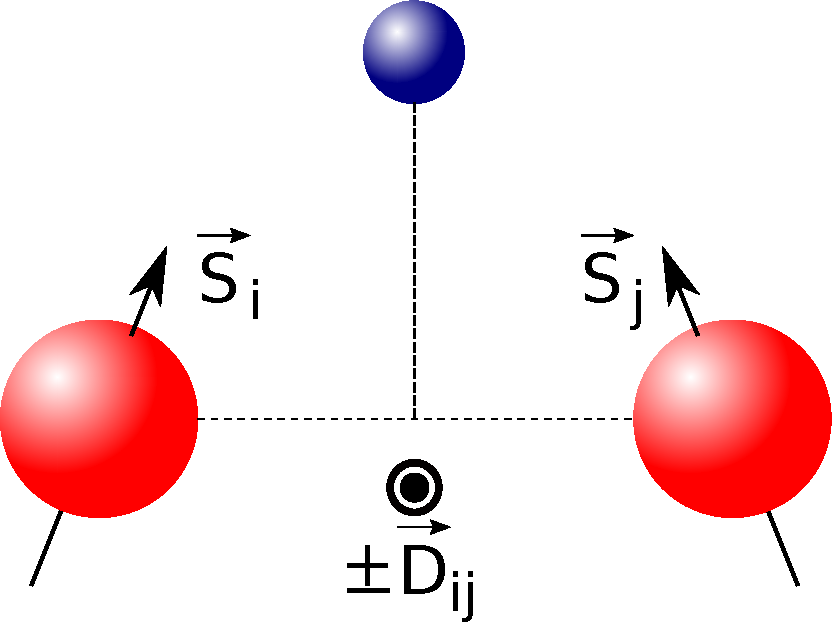
\includegraphics[width=0.6\textwidth]{Figures/InterfacialDMI.pdf} 
%\caption{An illustration of the geometry of an interfacial DMI. The antisymmetric interaction between the spins $\mathbold{S}_i$ and $\mathbold{S}_j$ is mediated by a third magnetic particle in blue. The direction of $\mathbold{D}_{ij}$ is then perpendicular to the plane spanned by the three particles.}
%\label{fig:InterfacialDMI} 
%\end{center}
%\end{figure}
\begin{figure}[h!]
\centering
\begin{tikzpicture}
\node[above right] (img) at (0,0) {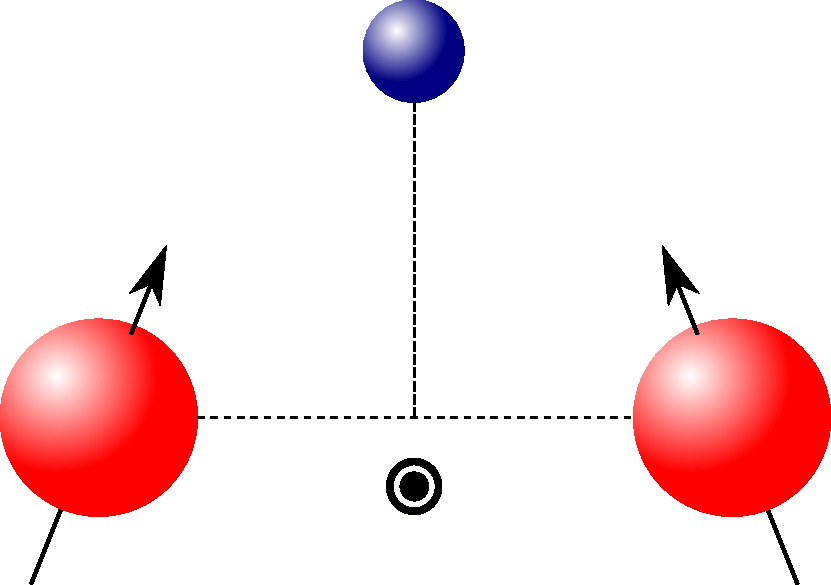
\includegraphics[width=0.6\textwidth]{Figures/InterfacialDMIv2}};
\node at (70pt,110pt) {\Large{$\mathbold{S}_i$}};
\node at (210pt,110pt) {\Large{$\mathbold{S}_j$}};
\node at (140pt,10pt) {\Large{$\pm\mathbold{D}_{ij}$}};
\end{tikzpicture}
        \caption{An illustration of the geometry of an interfacial DMI. The antisymmetric interaction between the spins $\mathbold{S}_i$ and $\mathbold{S}_j$ is mediated by a third magnetic particle in blue. The direction of $\mathbold{D}_{ij}$ is then perpendicular to the plane spanned by the three particles.}
        \label{fig:InterfacialDMI}
\end{figure}
We now assume that the magnetic particles with spins $\mathbold{S}_i$ and $\mathbold{S}_j$ are located in the $xy$-plane, and that the mediating magnetic particle of a different type lies above them. According to symmetry, the vector $\mathbold{D}_{ij}$ is then given by $\mathbold{D}_{ij} = D/a\mathbold{\hat{y}}$ if $i$ and $j$ are nearest neighbours in the $x$-direction, and $\mathbold{D}_{ij} = -D/a\mathbold{\hat{x}}$ if $i$ and $j$ are nearest neighbours in the $y$-direction. Here $a$ is the lattice constant and $D$ a constant that can be both positive and negative. We have for simplicity assumed an equal interaction in all directions in the $xy$-plane. Using this result, we explicitly derive the expression for the interfacial DMI energy density for reasons we will see in Section \ref{sec:Parity}. As the spin can be written in terms of the magnetization as $\mathbold{S} = -\mathbold{M}S/M_s$, the Dzyaloshinskii--Moriya Hamiltonian can be written as
\begin{align}
    H_{DM} = \frac{1}{M_s^2}\sum_{\langle i,j\rangle} \mathbold{D}_{ij}\cdot\left( \mathbold{M}_i\times\mathbold{M}_j\right)
\end{align}
where the $S^2$ has been included in the magnitude of $\mathbold{D}_{ij}$. As mentioned earlier, we can do a Taylor expansion of the magnetization as it is a continious function in the micromagnetic model. To first order this Taylor expansion becomes
\begin{align}
    \mathbold{M}_{i+1} \approx \mathbold{M}_i + a\frac{\partial\mathbold{M}_i}{\partial x}
\end{align}
in the $x$-direction. An entirely equivalent expansion can also be done in the $y$-direction. The expansion in the $z$-direction is ignored as $\mathbold{D}_{ij}$ does not have a $z$-component. The energy density can then be calculated to be
\begin{subequations}
\begin{align}
\nonumber\epsilon_{DM}^{\textrm{(interface)}} &= 
\frac{D}{M_s^2}\left[\hat{y}\cdot\left(\mathbold{M}\times\frac{\partial\mathbold{M}}{\partial x}\right) - \hat{x}\cdot\left(\mathbold{M}\times\frac{\partial\mathbold{M}}{\partial y}\right)\right] \\
\nonumber&= \frac{D}{M_s^2} \bigg[\left(M_z\frac{\partial M_x}{\partial x} - M_x \frac{\partial M_z}{\partial x}\right)(\mathbold{\hat{y}}\cdot(\mathbold{\hat{z}}\times\mathbold{\hat{x}}))\\
\label{eq:DMInterfaceCrossP}
&\hspace{10.4mm}- \left(M_y\frac{\partial M_z}{\partial y} - M_z \frac{\partial M_y}{\partial y}\right)(\mathbold{\hat{x}}\cdot(\mathbold{\hat{y}}\times\mathbold{\hat{z}}))\bigg] \\
\label{eq:DMInterface}
&= \frac{D}{M_s^2}\left[M_z(\mathbold{\nabla}\cdot\mathbold{M})-(\mathbold{M}\cdot\mathbold{\nabla})M_z\right].
\end{align}
\end{subequations}
The observant reader may have noticed that both the Rashba spin-orbit coupling and Dzyaloshinskii-Moriya interaction occur in materials with inversion asymmetry. Dzyaloshinskii first introduced DMI based on a phenemenological reasoning \citep{Dzyaloshinskii1958} to describe what had been observed experimentally, and Moriya later proposed that the microscopic mechanism behind this was spin-orbit coupling \cite{Moriya1960}. In thin-film system it is then reasonable to assume that Rashba spin-orbit coupling can be the mechanism behind DMI. This was in fact shown mathematically by Kim \textit{et al.} \citep{DMIfromRashba_Kim}. They started with the model Hamiltonian
\begin{align}
H = H_{\textrm{kin}} + H_R + H_E = \frac{\mathbold{p}^2}{2m_e} + \frac{\alpha_R}{\hbar}\mathbold{\sigma}\cdot(\mathbold{p}\times\mathbold{\hat{n}}) + J\mathbold{\sigma}\cdot\mathbold{\hat{M}}
\end{align}
that includes the kinetic energy of electrons confined to a plane, a Rashba spin-orbit coupling and the symmetric exchange energy between the spins. A unitary transformation was then performed on the Hamiltonian to remove the explicit Rashba Hamiltonian from the model, so that the transformed Hamiltonian could be written as $H' = U^{\dagger} H U = H_{\textrm{kin}} + H_E' + \orderof(\alpha_R^2)$. This unitary transformation, defined by
\begin{align}
U = \exp\left[-i\frac{\alpha_R m_e}{\hbar^2}\mathbold{\sigma}\cdot(\mathbold{r}\times\mathbold{\hat{n}})\right],
\end{align}
does not change the eigenvalues of the system, and the physics in the transformed Hamiltonian is therefore the same as the original model Hamiltonian. It was then shown that the transformed symmetric exchange energy included an interfacial DMI term with the strength of the parameter $D$ being
\begin{align}
\label{eq:DalphaR}
D = \frac{4\alpha_Rm_e A}{\hbar^2}.
\end{align}

\subsection{Pinning potentials}
With the exception of the RKKY interaction and voltage induced magnetic anisotropy, the free energy terms discussed so far are not explicitly dependent on position, but rather dependent on the magnetization profile $\mathbold{M}(\mathbold{r})$. If we were then to consider a system where the RKKY interaction and voltage induced magnetic anisotropy do not contribute to the free energy, and only the remaining energy terms discussed do, a given magnetization pattern $\mathbold{M}(\mathbold{r})$ will have the same free energy independent of where in the material it is localized. In other words, $\mathbold{M}(\mathbold{r})$ and $\mathbold{M}(\mathbold{r}-\mathbold{r}_0)$ have the same energy for any choice of $\mathbold{r}_0$. However, a realistic material will have impurities, and with the impurities local energy variations that are known as pinning centers appear. These pinning centers can make a certain position in the material for a magnetization pattern such as a domain wall or a magnetic skyrmion (a magnetization pattern that we will discuss in the next chapter) more energetically favorable to be localized. When considering the dynamics of magnetization patterns that are pinned in these pinning centers, one will need to supply a certain amount of energy for the magnetization pattern to move across the energy barrier that keeps the pattern localized in the pinning center (FIND CITATION). There are several mechanisms that can cause these local energy variations to occur. In \cite{LiuLi2013} Liu and Li proposed that by modifying the local density of itinerant electrons the exchange stiffness $A$ and DMI strength $D$ could become spatially dependent. When this is done the free energy becomes explicitly dependent on position, and due to the damping in the system any magnetization pattern will relax to its local minimum in the free energy. Another way to introduce pinning centers is to have spatial variations in the perpendicular magnetic anisotropy. This can be realized by having notches in the surface of the magnetic material \cite{Sampaio2013}. It is also possible to have pinning centers in the material by having a hole in the magnetic material \cite{Muller2015}, where for example certain atoms in a crystalline magnetic material are removed or replaced by non-magnetic atoms. 

\section{The Landau--Lifshitz--Gilbert equation}
The key equation in the micromagnetic model is the Landau--Lifsthitz--Gilbert equation, which is based on the behavior of magnetic moments in magnetic fields. Magnetic moments are known to precess around magnetic fields when they are not perfectly aligned. This is known as Larmor precession. The magnetization in a magnet will therefore also perform Larmor precession, as the magnetization is the magnetic moment in a unit volume. This precession can be described by
\begin{align}
\frac{\textrm{d}\mathbold{M}}{\textrm{d}t} = -\gamma\mathbold{M}\times\mathbold{H},
\end{align}
where $\gamma$ is the gyromagnetic ratio defined by
\begin{align}
\gamma = \frac{g_e\mu_0\mu_B}{\hbar}
\end{align}
where $g_e \approx 2$ is the $g$-factor, $\mu_0$ the vacuum permeability and $\mu_B$ is the Bohr magneton. In addition to performing a precessing motion around the magnetic field, the magnetization will eventually relax parallel to the field to minimize the energy of the system. This can be modeled by introducing a damping term that is perpendicular to the magnetization and the precession of the magnetization. The precessional and damped precessional motions are illustrated in Figure \ref{fig:Precessions}. Originally Landau and Lifshitz proposed \cite{LandauLifshitz1935} a damping term of the form
\begin{align}
\frac{\textrm{d}\mathbold{M}}{\textrm{d}t} = -\gamma\mathbold{M}\times(\mathbold{H}+\frac{\alpha}{M_s}\mathbold{M}\times\mathbold{H}),
\end{align}
but it was discovered that this did not agree well with experiments in systems with a large damping parameter $\alpha$. Therefore Gilbert proposed a damping term that included the time-derivative of the magnetization instead \cite{Gilbert2004Classics}, which agreed much better with experiments \cite{GilbertKelly1955}, of the form
\begin{align}
\label{eq:LLG}
\frac{\textrm{d}\mathbold{M}}{\textrm{d}t} = -\gamma\mathbold{M}\times\mathbold{H}+\frac{\alpha}{M_s}\mathbold{M}\times\frac{\textrm{d}\mathbold{M}}{\textrm{d}t}.
\end{align}
This is known as the Landau--Lifshitz--Gilbert equation, and is the equation that governs the dynamics in the micromagnetic model.
\begin{figure}[h!]
\centering
\begin{subfigure}{.3\textwidth}
  \centering
  \begin{tikzpicture}
\node[above right] (img) at (0,0) {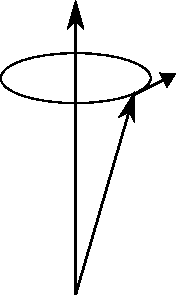
\includegraphics[width=0.7\textwidth]{Figures/Precessionv2}};
\node at (85pt,90pt) {\Large{$\mathbold{M}$}};
\node at (110pt,140pt) {\Large{$-\gamma\mathbold{M}\times\mathbold{H}$}};
\node at (20pt,150pt) {\Large{$\mathbold{H}$}};
\end{tikzpicture}
  \caption{}
\end{subfigure}%
\hspace{1cm}
\begin{subfigure}{.33\textwidth}
  \centering
  \begin{tikzpicture}
\node[above right] (img) at (0,0) {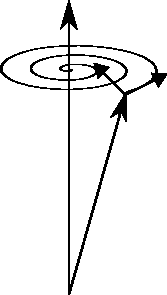
\includegraphics[width=0.6\textwidth]{Figures/DampedPrecessionv2}};
\node at (85pt,90pt) {\Large{$\mathbold{M}$}};
\node at (110pt,140pt) {\Large{$-\gamma\mathbold{M}\times\mathbold{H}$}};
\node at (-10pt,100pt) {\Large{$\alpha\mathbold{M}\times\partial_t\mathbold{M}$}};
\node at (20pt,150pt) {\Large{$\mathbold{H}$}};
\end{tikzpicture}
  \caption{}
\end{subfigure}
\caption{The precession of the magnetization vector around a magnetic field. In \textbf{(a)} the precession is undamped and so the magnetization performs counter-clockwise circular rotations around the magnetic field. In \textbf{(b)} the damping component pointing towards the magnetic field causes a spiralling motion of the magnetization vector that eventually aligns the magnetization with the magnetic field.}
\label{fig:Precessions}
\end{figure}
It should be noted that the magnetic field $\mathbold{H}$ that the magnetization precesses around is not only an external magnetic field applied to the system, but it is the effective magnetic field experienced locally by the magnetization. The direction of this magnetic field represents the direction in which the magnetization will have a minimum in the micromagnetic energy, and the effective field can therefore be written in terms of the micromagnetic energy. The effective field in the absence of an external field is given by
\begin{align}
\label{eq:EffectiveField}
\nonumber\mathbold{H}_{\textrm{eff}} &= -\frac{1}{\mu_0}\frac{\delta\epsilon[\mathbold{M}]}{\delta\mathbold{M}} \\
&= \frac{2A}{\mu_0M_s}\mathbold{\nabla}^2\mathbold{m}+\frac{2(K+\eta E)}{\mu_0M_s}m_z\mathbold{\hat{z}} + \frac{2D}{\mu_0M_s}\left(\frac{\partial m_z}{\partial x}\mathbold{\hat{x}}+\frac{\partial m_z}{\partial y}\mathbold{\hat{y}}-(\mathbold{\nabla}\cdot\mathbold{m})\mathbold{\hat{z}}\right),
\end{align}
with $\mathbold{m}$ being a unit vector in the direction of the magnetization. Here the symmetric exchange interaction, perpendicular and voltage induced magnetic anisotropy and interfacial DMI have been taken into consideration in the effective field.

Another thing to notice about the LLG equation is that only the direction of the magnetization $\mathbold{M}$ and not its magnitude changes with time. This can be seen by multiplying \eqref{eq:LLG} by $\mathbold{M}$ from the left:
\begin{align}
\mathbold{M}\cdot\frac{\textrm{d}\mathbold{M}}{\textrm{d}t} = \frac{1}{2}\frac{\textrm{d}}{\textrm{d}t} \mathbold{M}^2 =  \mathbold{M}\cdot\left(-\gamma\mathbold{M}\times\mathbold{H}+\frac{\alpha}{M_s}\mathbold{M}\times\frac{\textrm{d}\mathbold{M}}{\textrm{d}t}\right) = 0.
\end{align}
In other words the LLG equation conserves the magnitude of the magnetization, meaning $\frac{\textrm{d} M_s}{\textrm{d}t} = 0$.

\section{Spin-transfer torques}
The LLG equation presented in \eqref{eq:LLG} describes the dynamics of magnetic moments in the presence of external magnetic fields and internal effective fields that try to minimize the energy of the system. However, there are also other means of inducing dynamics of the magnetization in a material. The LLG equation can be extended to include these effects by adding torques to the right hand side of the equation (note that these torques will not have the same units as a mechanical torque, but the effect is well described by the term torque as it appears as a rotation of the magnetization direction). One method that has shown promise in inducing magnetization dynamics is the spin-transfer torque. In \cite{Berger1978} Berger noted that when you apply a current through a magnetic domain wall, the main effect was not a scattering of the electrons, but that the domain wall tended to follow the motion of the electrons. When a spin-polarized current is passing through a magnetic material, the conduction electrons will want to align their magnetic moments with the local magnetization in the material to reduce their energy. The way the electrons reach a lower energy state is by the torque acting on them from the local magnetization due to the fact that they are not aligned (or anti-aligned). Since the conduction electrons experience a torque when passing through a magnetization not parallel to their own magnetic moments, Newton's third law dictates that there must be an equal and opposite torque acting on the local magnetization. In other words, through a means of conserving angular momentum the conduction electrons transfer some of their spin to the local magnetization, hence the term spin-transfer torque (STT). Slonczewski introduced this torque in the LLG equation for the case of STT acting on a magnetic multilayer system \cite{Slonczewski1996}. This torque was observed experimentally a few years after the publications by Berger and Slonczewski \cite{Tsoi1998,Myers1999}.

\subsection{Adiabatic spin-transfer torque} \label{sec:AdSTT}
To start off the introduction of spin-transfer torques we will first discuss them qualitatively in what is known as the adiabatic regime. In this regime it is assumed that the magnetic moments of the conduction electrons passing through the magnetic material relaxes fast enough to always follow the local magnetization. If we then consider a current passing through a magnetic layer with a magnetization direction $\mathbold{m}_i = \mathbold{M}_i/M_s$, the magnetic moment of the electrons will be parallel to $\mathbold{m}_i$. Not long after passing through $\mathbold{m}_i$, the electrons pass through another magnetic material with a magnetization direction $\mathbold{m}_j$ which is tilted with respect to $\mathbold{m}_i$. Since the electrons have a magnetic moment that is not aligned with $\mathbold{m}_j$, this magnetization will lead to a torque acting on the conduction electrons to make their magnetic moments relax to be aligned with $\mathbold{m}_j$ instead of $\mathbold{m}_i$. As we mentioned earlier, there is then an equal torque acting on $\mathbold{m}_j$ in the opposite direction, attempting to align it with the magnetic moment of the electrons, which is $\mathbold{m}_i$ at the time of incidence. If we then assume that the magnitude of $\mathbold{m}_i$ and $\mathbold{m}_j$ are equal, the torque acting on $\mathbold{m}_j$ must then be proportional to the component of $\mathbold{m}_i$ which is perpendicular to $\mathbold{m}_j$. This means that the torque is proportional to $\mathbold{m}_i-(\mathbold{m}_i\cdot\mathbold{m}_j)\mathbold{m}_j$, as illustrated in Figure \ref{fig:AdSTT}.
%\begin{figure}[h!]
%  \centering
%  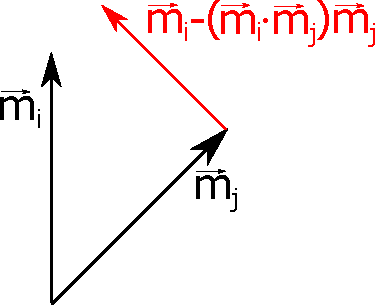
\includegraphics[width=0.4\linewidth]{Figures/AdiabaticSTT}
%\caption{The adiabatic spin-transfer torque acting on a magnetic moment $\mathbold{m}_j$ from a spin-polarized current having passed through the magnetic moment $\mathbold{m}_i$ is proportional to the component of $\mathbold{m}_i$ perpendicular to $\mathbold{m}_j$.}
%\label{fig:AdSTT}
%\end{figure}

\begin{figure}[h!]
\centering
\begin{tikzpicture}
\node[above right] (img) at (0,0) {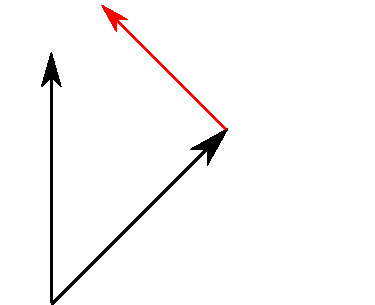
\includegraphics[width=0.4\textwidth]{Figures/AdiabaticSTTv2}};
\node at (5pt,110pt) {\Large{$\mathbold{m}_i$}};
\node at (120pt,60pt) {\Large{$\mathbold{m}_j$}};
\node at (150pt,140pt) {\textcolor{red}{\Large{$\mathbold{m}_i-\left(\mathbold{m}_i\cdot\mathbold{m}_j\right)\mathbold{m}_j$}}};
\end{tikzpicture}
        \caption{The adiabatic spin-transfer torque acting on a magnetic moment $\mathbold{m}_j$ from a spin-polarized current having passed through the magnetic moment $\mathbold{m}_i$ is proportional to the component of $\mathbold{m}_i$ perpendicular to $\mathbold{m}_j$.}
        \label{fig:AdSTT}
\end{figure}

This discussion was for two discrete magnetic moments. Let us now consider a case where the magnetization in a material varies slowly in a way that can be described by a function of position, such as a magnetic domain wall. We can still use the result from before, but instead of $\mathbold{m}_j$ being a magnetic moment in a direction independent of the direction of $\mathbold{m}_i$, there is only an infinitesimal change in $\mathbold{m}_j$ from $\mathbold{m}_i$. So when the electrons arrive at the magnetization at a position $x+\d x$ (here assuming the electrons flow in the positive $x$-direction), their magnetic moment are aligned with the magnetization at the position $x$. Since the magnetization varies slowly, we can do a Taylor expansion to approximate the magnetization at position $x+\d x$ as a function of the magnetization at position $x$:
\begin{align}
    \mathbold{m}(x+\d x) \approx \mathbold{m}(x) + \d x\partial_x \mathbold{m}(x).
\end{align}
Typically $\d x$ would be on the length scale of the lattice constant. Using this expansion we can then find the direction of the torque acting on the magnetization at $x+\d x$ from the current which has a polarization along the magnetization at $x$:
\begin{align}
\nonumber&\hspace{5.5mm}\mathbold{m}(x)-\left[\mathbold{m}(x)\cdot\mathbold{m}(x+\d x)\right]\mathbold{m}(x+\d x) \\
\nonumber&\approx \mathbold{m}(x)-\left[1 + \d x \mathbold{m}(x)\cdot\partial_x \mathbold{m}(x)\right]\left[\mathbold{m}(x) + \d x\partial_x \mathbold{m}(x)\right] \\
&= -\d x \partial_x \mathbold{m}(x). \label{eq:DiffSTTterm}
\end{align}
Here we have used that $\mathbold{m}(x)\cdot\partial_x \mathbold{m}(x) = 0$ as the magnitude of $\mathbold{m}$ is assumed to be constant for all positions. As we can see the result is somewhat different than for the two discrete magnetic moments as we have a differential in the torque, but the physical interpretation of the result is still the same. When the magnetic moments of the conduction electrons follow the local magnetization, their magnetic moment is adjusted from $\mathbold{m}(x)$ to $\mathbold{m}(x) + \d x \partial_x \mathbold{m}(x)$. The direction of the torque acting on the magnetization at $x +\d x$ must then be in the opposite direction of this change, along $-\d x \partial_x \mathbold{m}(x)$. Remember that what we have discussed so far has only been the direction of the torque acting on the local magnetization, and not its magnitude. A pre-factor must then be included that reflects how much spin is transferred from each electron to the local magnetization, the frequency of each electron passing through the magnetization, and how many of these electrons that are polarized of the magnetization at the previous position. Each electron has a magnetic moment $\mathbold{\mu} = \mu_B \mathbold{m}$, with $\mathbold{m}$ being a unit vector in the direction of the magnetization. The frequency of the electrons passing through the magnetization can be expressed in terms of the current, and since the magnetization is a volume average of the magnetic moments in the material, we want the current density to describe the rate of change to the magnetization. Letting the current passing through per cross-sectional area be $j$, the current density is $j/d_j$ with $d_j$ being the thickness of the material with magnetization $\mathbold{M}_j$. Assuming a portion $P$ of the electrons in the current are polarized, the frequency of each electron transferring its magnetic moment to the magnetic material per volume unit is $jP/(-ed)$, where we have divided the current by its charge carrier. The adiabatic spin-transfer torque acting on a magnetization $\mathbold{M}_j$ after a current passing through a magnetization $\mathbold{M}_i$ is then
\begin{align}
    \mathbold{T}_{STT}^{\textrm{(adiabatic)}} = -\frac{\mu_B j P}{e d_j} (\mathbold{m}_i-(\mathbold{m}_i\cdot\mathbold{m}_j)\mathbold{m}_j)
    = -\frac{\gamma \hbar jP}{2 e \mu_0 d}\mathbold{m}_j\times\left(\mathbold{m}_i\times\mathbold{m}_j\right).
    \label{eq:STT_Adiabatic_Macro}
\end{align}
In a material with a slowly varying magnetization, the thickness of the magnetization goes from $d_j$ to $\d x$. Using the expression found in \eqref{eq:DiffSTTterm} and that the current is moving in the direction $\mathbold{\hat{j}}$, the adiabatic STT in this case becomes
\begin{align}
 \mathbold{T}_{STT}^{\textrm{(adiabatic)}} = \frac{\mu_B j P}{e M_s} (\mathbold{\hat{j}}\cdot\mathbold{\nabla})\mathbold{M}(\mathbold{r}). \label{eq:AdSTTnonuniform}
\end{align}
These torques can then be included in the right hand side of the LLG equation in \eqref{eq:LLG} to describe the dynamics of adiabatic STTs.

\subsection{General spin-transfer torque} \label{sec:GeneralSTT}
So far we have discussed how STT terms would appear in the LLG equation if the magnetic moments of the conduction electrons follow the local magnetization adiabatically. We will now derive the STT terms for a slowly varying magnetization more rigidly based on the spin continuity equation. This will be done for a more general case where the magnetic moments of the conduction electron can have a small component perpendicular to the local magnetization. This derivation mainly follows the derivation by Zhang and Li \cite{ZhangLi-04}. We start by considering the spin continuity equation, given by
\begin{align}
\partial_t\mathbold{s} + \mathbold{\nabla}\hat{J} = \frac{1}{i\hbar} \left[\mathbold{s}, H_{sd}\right] - \Gamma(\mathbold{s}).
\end{align}
Here $\mathbold{s}$ is the spin operator for the conduction electrons, $\hat{J}$ the spin-current operator, $\Gamma(\mathbold{s})$ the relaxation rate of the conduction electrons due to scattering, and $H_{sd}$ the s-d Hamiltonian
\begin{align}
H_{sd} = -J_{\textrm{ex}}\mathbold{s}\cdot\mathbold{S}
\end{align}
which describes the (anti)ferromagnetic coupling between the itinerant spins $\mathbold{s}$ and local spins $\mathbold{S}$ depending on the sign of the coupling strength $J_{\textrm{ex}}$. In the micromagnetic model we are in a semi-classical limit, and we will therefore not treat the local spins quantum mechanically as operators, but as expectation values. The spins of the conduction electrons, however, we will still treat as operators for now. We proceed by calculating the commutator
\begin{align}
\left[\mathbold{s}, H_{sd}\right]_i = -J_{\textrm{ex}} \left[s_i, s_j S_j\right] = -J_{\textrm{ex}}\left[s_i, s_j\right] S_j.
\end{align}
Here we assume the Einstein summation convention. Note that $S_j$ can be pulled out of the commutators as it is not treated as an operator. The spin operators satisfy the commutation relation
\begin{align}
\left[s_i, s_j\right] = i\hbar\varepsilon_{ijk}s_k,
\end{align}
which can be obtained from the Pauli matrix commutation relation as $s_i = \hbar \sigma_i/2$. We then find that
\begin{align}
\frac{1}{i\hbar}\left[\mathbold{s}, H_{sd}\right] = -J_{\textrm{ex}}\mathbold{S}\times\mathbold{s}.
\end{align}
From now on we will also treat the remaining operators as expectation values. We make the ansatz that the spin density $\mathbold{m}$ of the conduction electrons are mainly parallel to the local magnetization $\mathbold{M}$, but allow a small perpendicular component $\delta\mathbold{m}$:
\begin{align}
    \mathbold{m} = \langle\mathbold{s}\rangle = \frac{m_0}{M_s} \mathbold{M} + \delta\mathbold{m}.
\end{align}
Note here that the ratio $m_0/M_s$ is very small, as the magnetization of the current is far below saturation. Moving on to the expectation value of the spin-current, we can write this as a tensor product between the velocity of the electrons, and their spin: $\langle\hat{J}\rangle = \mathbold{v}\otimes\mathbold{s}$. Instead of writing this expectation value in terms of the velocity $\mathbold{v}$ and spin $\mathbold{s}$, we want to write it in terms of the current density and magnetization. Using that $\mathbold{s} \approx \mu_B\mathbold{M}/M_s$ and following a similar approach as in the last section to rewrite the velocity in terms of the current $j$ per unit area, we find that
\begin{align}
\langle\hat{J}\rangle = -\frac{\mu_B P}{eM_s} \mathbold{j}\otimes\mathbold{M}.
\end{align}
Note that here we have assumed the spin current is adiabatic. To be exact one needs to include a non-adiabatic spin-current term $\delta\langle\hat{J}\rangle$, but it is assumed this is negligible. The product $\mathbold{\hat{\nabla}}\langle\hat{J}\rangle$ in the spin continuity equation then becomes
\begin{align}
\mathbold{\hat{\nabla}}\langle\hat{J}\rangle = -\frac{\mu_B P}{e M_s}\left(\mathbold{j}\cdot\mathbold{\nabla}\right)\mathbold{M}
\end{align}
when one assumes a uniform charge current density $\mathbold{j}$. Lastly, we approximate the relaxation rate due to scattering $\Gamma(\mathbold{s})$ by the expectation value 
\begin{align}
\langle\Gamma(\mathbold{s})\rangle \approx \frac{\delta\mathbold{m}}{\tau_{\textrm{sf}}},
\end{align}
with $\tau_{\textrm{sf}}$ being the spin-flip relaxation time. The spin continuity equation then becomes
\begin{align}
\partial_t\mathbold{m} -\frac{\mu_B P}{e M_s}\left(\mathbold{j}\cdot\mathbold{\nabla}\right)\mathbold{M} =   -\frac{J_{\textrm{ex}} S}{M_s}\mathbold{m}\times\mathbold{M} - \frac{\delta\mathbold{m}}{\tau_{\textrm{sf}}} =    -\frac{1}{\tau_{\textrm{ex}}M_s}\delta\mathbold{m}\times\mathbold{M} - \frac{\delta\mathbold{m}}{\tau_{\textrm{sf}}} \label{eq:SpinContinuityEq}
\end{align}
where we have introduced the spin relaxation $\tau_{\textrm{ex}} = (J_{\textrm{ex}}S)^{-1}$ time due to the exchange interaction. The first term appearing on the right hand side is a torque acting on the spin of the electrons due to an interaction with the local magnetization. As we have discussed earlier, Newton's third law then dictates that there must be an equal torque acting on $\mathbold{M}$ in the opposite direction, leaving us with the spin-transfer torque
\begin{align}
\mathbold{T}_{STT} = \frac{1}{\tau_{\textrm{ex}}M_s}\delta\mathbold{m}\times\mathbold{M}.
\end{align}
To determine this torque we must first find $\delta\mathbold{m}$. We can do this based on \eqref{eq:SpinContinuityEq}, but first we find an expression for $\delta \mathbold{m} \times \mathbold{M}$, which we can obtain by taking the cross product of \eqref{eq:SpinContinuityEq} with $\mathbold{M}$ from the right. We then find that
\begin{align}
\delta\mathbold{m}\times\mathbold{M} = \tau_{\textrm{sf}}\left[\frac{m_0}{M_s}\mathbold{M}\times\partial_t\mathbold{M} - \frac{\mu_B P}{e M_s} \mathbold{M}\times(\mathbold{j}\cdot\mathbold{\nabla})\mathbold{M} + \frac{M_s}{\tau_{\textrm{ex}}}\delta\mathbold{m} \right]
\end{align}
where we have neglected the time derivative of $\delta\mathbold{m}$. Inserting the expression for $\delta\mathbold{m}$ from \eqref{eq:SpinContinuityEq} into the expression above, we finally find that the total spin-transfer torque becomes
\begin{align}
\mathbold{T}_{STT} = \frac{1}{1+\beta^2} \left[ \frac{\beta m_0}{M_s^2}\mathbold{M}\times\partial_t\mathbold{M} - \frac{m_0}{M_s} \partial_t\mathbold{M} + \frac{\mu_B P}{e M_s} (\mathbold{j}\cdot\mathbold{\nabla})\mathbold{M} - \frac{\beta \mu_B P}{e M_s^2} \mathbold{M}\times(\mathbold{j}\cdot\mathbold{\nabla})\mathbold{M}\right],
\end{align}
where we have introduced the ratio $\beta = \tau_{\textrm{ex}}/\tau_{\textrm{sf}}$. The first two terms on the right hand side are of a form that already appear in the LLG equation, and introduce no new physics. In addition, they are proportional to $m_0/M_s$, and are therefore negligible. The third term we recognize being the adiabatic STT term in \eqref{eq:AdSTTnonuniform} that we found in the previous section, with an additional factor $(1+\beta^2)^{-1}$. The last term is of particular interest, as it is on a form that we have not seen before. As we can see, the term is perpendicular to the adiabatic STT and contains an additional factor $\beta$. In the adiabatic regime, which we considered in the previous section, $\beta \rightarrow 0$ as the spin-flip relaxation time is much greater than the exchange relaxation time when the conduction electrons follow the local magnetization adiabatically. The last term therefore only appears when we are not in the adiabatic regime, and is therefore called the non-adiabatic STT. This torque, which is caused by the magnetic moments of the itinerant electrons that are not aligned with the local magnetization, will twist the magnetization out of the plane spanned by the magnetization in that area. 


%\section{Spin-Hall effect}

%\section{Spin orbit torques}

%\section{Rashba spin-orbit coupling}

%\section{Magnons}

\chapter{Skyrmions, their symmetries and dynamics} \label{chap:Skyrmions}
The micromagnetic model introduced in the previous chapter is able to describe many different magnetization patterns that are static solutions of the LLG equation, one of them being magnetic skyrmions which we will introduce in this chapter. Here we will discuss their topology, what mechanisms are needed to stabilize them, and symmetry considerations of both the skyrmion profile and the LLG equation. Moreover, we will introduce the Thiele equation, which is a simplification of the LLG equation under the ansatz that the skyrmion moves rigidly. The Thiele equation is an algebraic vector equation in the velocity components of the skyrmion, making it much easier to solve than the LLG equation which is a partial differential equation. We also touch upon the subject of Berry phases and the topological Hall effect to describe some of the dynamical properties of skyrmions, but save the full analytical and numerical solution of the skyrmion velocity for Chapter \ref{chap:SkyrmionDynamics}.

\section{Skyrmions} \label{sec:Skyrmions}
In certain types of materials, such as chiral magnets, an exotic magnetization pattern has been found to occur. This magnetization pattern, known as a skyrmion, is a vortex-like magnetization structure with non-trivial topology. The term skyrmion originates from the physicist Tony Skyrme, who described baryons and mesons as topological solitons \cite{Skyrme1962}. While Skyrme had nothing to do directly with magnetic skyrmions, which we consider in this thesis, his name was used because the skyrmion has a non-trivial topology and is therefore also a topological soliton. By a non-trivial topology we mean that the magnetization of the skyrmion wraps around the unit sphere, so that it has a non-zero skyrmion number \cite{Heinze2011}
\begin{align}
\label{eq:SkyrmionNumber}
N_{\textrm{sk}} = \frac{1}{4\pi}\int \mathbold{\hat{M}}\cdot(\partial_x \mathbold{\hat{M}} \times \partial_y \mathbold{\hat{M}}) \d x \d y.
\end{align}
Skyrmions have an integer skyrmion number, while vortices have a half-integer skyrmion number \cite{Tretiakov2007}. Skyrmions have been of particular interest in recent time, it was only first observed experimentally in 2009 \cite{Muhlbauer2009}. The reason for the interest for magnetic skyrmions in spintronics is that it has been shown skyrmions can be moved with a current density several orders of magnitude smaller than the critical current density needed to move magnetic domain walls \cite{Jonietz2010}. In addition, due to the non-trivial topology of the skyrmion, which acts as a knot in the magnetization, it will require a significant amount of energy to untie this knot and destroy the skyrmion, which makes it a stable information carrier. The information can be encoded by the direction of the magnetization in the skyrmion core, which can be up or down, and therefore acts as a bit. Skyrmions can also be useful for a compact data storage in form of skyrmion crystals \cite{Fert2013}, as the typical length-scale of skyrmions can be on the nanometer scale, depending on the stabilizing mechanism \cite{Nagaosa2013}. 

The magnetization of the skyrmion can be written in cartesian coordinates as
\begin{align}
\label{eq:SkyrmionMVec}
\mathbold{M}(\rho, \phi) = M_s
\begin{pmatrix}
\cos\Phi(\phi)\sin\theta(\rho) \\ \sin\Phi(\phi)\sin\theta(\rho) \\ \cos\theta(\rho)
\end{pmatrix}.
\end{align}
As the out-of-plane component (here the $z$-component) of the magnetization in the skyrmion is rotationally symmetric around the skyrmion's core, the out-of-plane angle $\theta$ can be written as a function of $\rho$ only, with $\rho$ being the distance to the skyrmion's core. The in-plane magnetization angle $\Phi$ is assumed to be a linear function of the azimuthal angle $\phi$, such that
\begin{align}
\Phi = m\phi + \psi.
\end{align}
An illustration of the angle $\Phi$ is shown in Figure \ref{fig:PhiFig}.
\begin{figure}[h!]
\centering
  \centering
    \begin{tikzpicture}
\node[above right] (img) at (0,0) {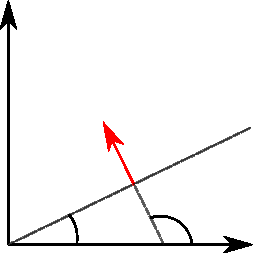
\includegraphics[width=0.4\textwidth]{Figures/SkyrmionAnglesv2}};
\node at (180pt,20pt) {\Large{$x$}};
\node at (20pt,180pt) {\Large{$y$}};
\node at (70pt,23pt) {\Large{$\phi$}};
\node at (140pt,35pt) {\Large{$\Phi$}};
\node at (80pt,110pt) {\textcolor{red}{\Large{$\left(m_x,m_y\right)$}}};
\end{tikzpicture}
\caption{The definitions of the angles $\Phi$ and $\phi$. In this case $\Phi = \phi+\pi/2$, in other words it can be described by $\Phi =m\phi+\psi$ with $m=1$ and $\psi=\pi/2$.}
\label{fig:PhiFig}
\end{figure}
Due to the periodical nature of the angles, $m$ is constrained to be an integer. The phase difference $\psi$ between $\Phi$ and $m\phi$ is a constant called the helicity of the skyrmion. If one plugs in the ansatz \eqref{eq:SkyrmionMVec} into \eqref{eq:SkyrmionNumber}, one finds that
\begin{align}
N_{\textrm{sk}} = \frac{m}{4\pi}\int_0^{2\pi}\d\phi \int_0^{\infty}\d \rho \sin\theta(\rho) \frac{\partial\theta(\rho)}{\partial\rho} = - \frac{m}{2} \cos(\theta(\rho))|_{(\rho = 0)}^{(\rho=\infty)}.
\end{align}
Unless $m$ is an even number, one must require that $\theta(\rho = 0) = 0$ and $\theta(\rho = \infty) = \pi$, or $\theta(\rho = 0) = \pi$ and $\theta(\rho = \infty) = 0$ for the skyrmion number to be an integer and not a half-integer.

The skyrmion needs a certain type of physical mechanism in the material to be a stable state. This mechanism will allow a lower energy state by having the neighbouring spins not be entirely parallel to each other, like the symmetric exchange interaction wants them to be. One of these mechanisms is the Dzyaloshinskii--Moriya interaction, which is the stabilizing mechanism of skyrmions we will consider in this thesis. Other mechanisms that can also cause the magnetic skyrmion to be a stable state are long-ranged magnetic dipolar interactions \cite{Lin1973}, frustrated exchange interactions \cite{Okubo2012} and four-spin exchange interactions \cite{Heinze2011}. If we consider the interfacial DMI energy density in \eqref{eq:DMInterface} and plug in our ansatz for the magnetization of the skyrmion, one finds that
\begin{align}
\epsilon_{DM}^{\textrm{(interface)}} = D\cos((m-1)\phi + \psi)\left(\frac{\partial\theta}{\partial\rho} + \frac{m}{\rho}\sin\theta\cos\theta\right).
\end{align}
For the DMI to have a net energy contribution, we must remove the dependence on $\phi$ as the average of a harmonic function over the plane will be zero. We therefore require that $m = 1$, which is not an even number, meaning we must apply the boundary conditions for $\theta(\rho)$ mentioned earlier. The helicity $\psi$ is then chosen to minimize the energy contribution from DMI, which leaves us with the two options $\psi = 0$ and $\psi = \pi$, depending on the sign of $D$ and the $\theta$ profile. Due to the boundary conditions for $\theta$, the magnetization in the core of the skyrmion points in the opposite direction of the magnetization far away from the skyrmion core. The magnetization direction far away from the core must therefore be a stable direction in the energy. This can be done in a system with an easy axis parallel to that direction. If we consider a skyrmion in a thin film, which makes sense with our choice of interfacial DMI, the easy axis must be perpendicular to that film. In other words, we need a thin-film system with perpendicular magnetic anisotropy. Finally, as our system is ferromagnetic, we also need to include the symmetric exchange interaction. This is also necessary if we want to treat the skyrmion in the micromagnetic model, where we assume that the magnetization can be estimated by a smooth function. This assumption was for example used in the Taylor expansion of the DMI Hamiltonian. Our model then has the energy density given by
\begin{align}
\nonumber \epsilon &= \epsilon_E + \epsilon_{PMA} + \epsilon_{DM}^{\textrm{(interface)}} \\
&=A \left[\left(\frac{\partial\theta}{\partial\rho}\right)^2 + \frac{\sin^2\theta}{\rho^2}\right] + K\sin^2\theta + D\cos\psi\left(\frac{\partial\theta}{\partial\rho} + \frac{\sin\theta\cos\theta}{\rho}\right),
\end{align}
assuming a magnetization profile given by \eqref{eq:SkyrmionMVec}. The energy is independent of $\phi$ due to our choice of $m$, but it remains a function of $\theta$ and $\rho$. As the skyrmion is a ground state, we can find the function $\theta(\rho)$ by minimizing the energy. Using the condition
\begin{align}
\frac{\delta\epsilon(\theta, \rho)}{\delta\theta(\rho)} = \frac{\partial\epsilon}{\partial\theta} - \frac{\textrm{d}}{\textrm{d}\rho} \frac{\partial\epsilon}{\partial (\frac{\partial\theta}{\partial \rho})} = 0
\end{align}
and introducing the dimensionless length $\tilde{\rho} = \rho D/A$, one ends up with the following differential equation for $\theta(\rho)$:
\begin{align}
\label{eq:ODEtheta}
\frac{\partial^2\theta}{\partial\tilde{\rho}^2} + \frac{1}{\tilde{\rho}}\frac{\partial\theta}{\partial\tilde{\rho}} - \frac{\sin\theta\cos\theta}{\tilde{\rho}^2}+\cos\psi\frac{\sin^2\theta}{\tilde{\rho}}-\frac{AK}{D^2}\sin\theta\cos\theta = 0.
\end{align}
Definining the ratio $AK/D^2$ as a parameter $C$, one can solve this equation numerically for a given $C$. Some numerical solutions are shown in Figure \ref{fig:ThetaProfile} when the boundary conditions $\theta(\rho = 0) = \pi$ and $\theta(\rho = \infty)$ have been used. It should be noted that this differential equation only has a solution when $\cos\psi = 1$ for the chosen boundary conditions. The solutions for the different helicities $\psi_1 = 0$ and $\psi_2 = \pi$ have a simple relation, however. This relation can be verified to be
\begin{align}
\label{eq:ThetaHelicityRelation}
\theta_{\psi_1}(\rho) = \pi - \theta_{\psi_2}(\rho),
\end{align}
as $\cos\psi$ is antisymmetric under a swap in helicities, and $\frac{\partial^2\theta}{\partial\tilde{\rho}^2}$, $\frac{\partial\theta}{\partial\tilde{\rho}}$, $\cos\theta_{\psi_i}$ are all antisymmetric under the relation above.
\begin{figure}[h!]
\begin{center}
\begin{tikzpicture}
\node[above right] (img) at (0,0)
{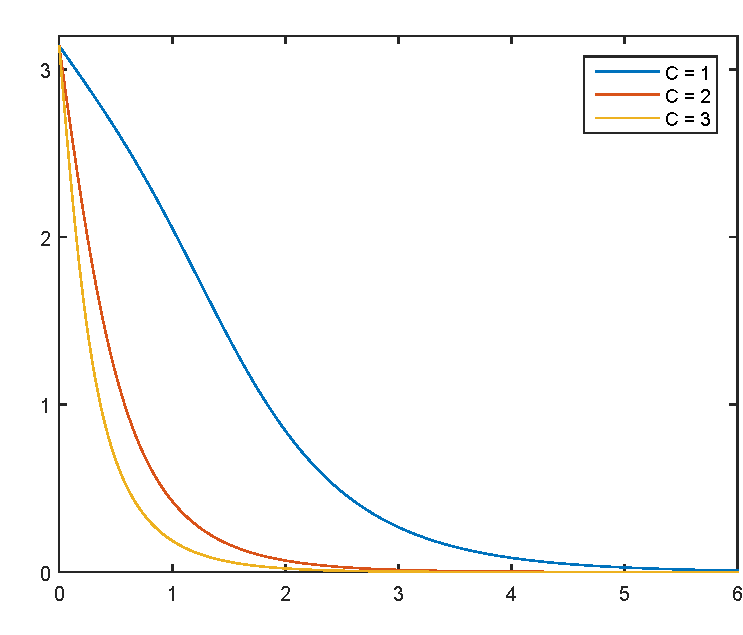
\includegraphics[width=0.6\textwidth]{Figures/SkyrmionRadialProfilesv2.pdf} };
 \node [right=of img,rotate=90,anchor=north,yshift=10.7cm,xshift=0.2cm] {$\theta(\tilde{r})$}; 
 \node at (150pt,10pt) {\Large{$\tilde{r}$}};
\end{tikzpicture}
%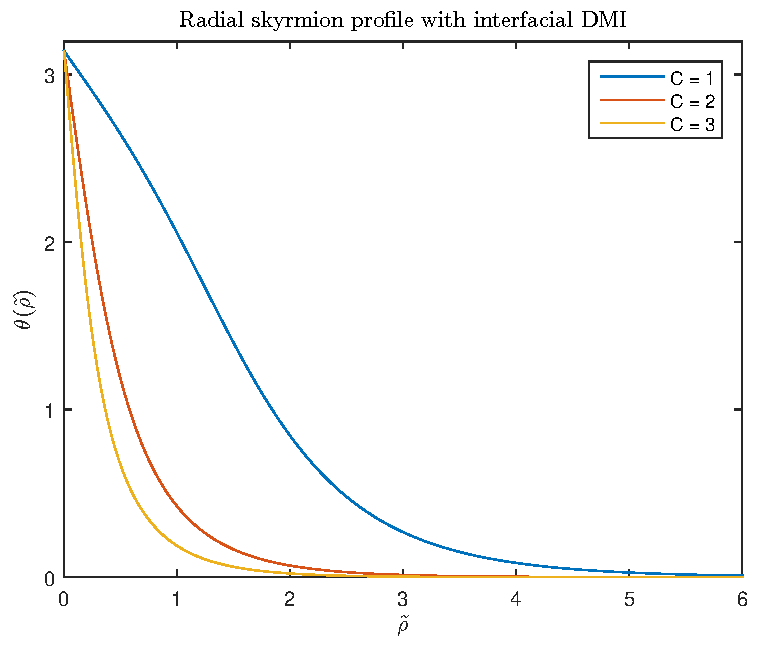
\includegraphics[width=0.6\textwidth]{Figures/SkyrmionRadialProfiles.pdf} 
\caption{The solution of the out-of-plane angle $\theta$ of the skyrmion profile for different values of $C$.}
\label{fig:ThetaProfile} 
\end{center}
\end{figure}
The two different skyrmions for the two different choices in helicities $\psi$ are illustrated in Figure \ref{fig:HedgehogSkyrmions}. This type of skyrmions is called a hedgehog skyrmion, due to the magnetization pattern that curves into or away from the core.
\begin{figure}[h!]
\centering
\begin{subfigure}{.49\textwidth}
  \centering
  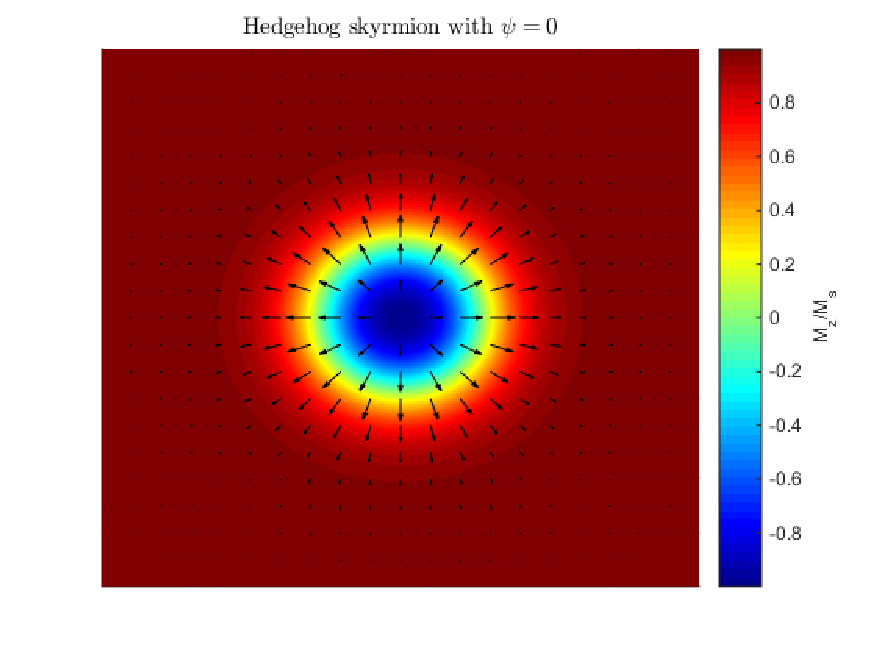
\includegraphics[width=\linewidth]{Figures/HedgehogSkyrmionPsi0.pdf}
  \caption{}
  \label{fig:HedgehogSkyrmion1}
\end{subfigure}
\begin{subfigure}{.49\textwidth}
  \centering
  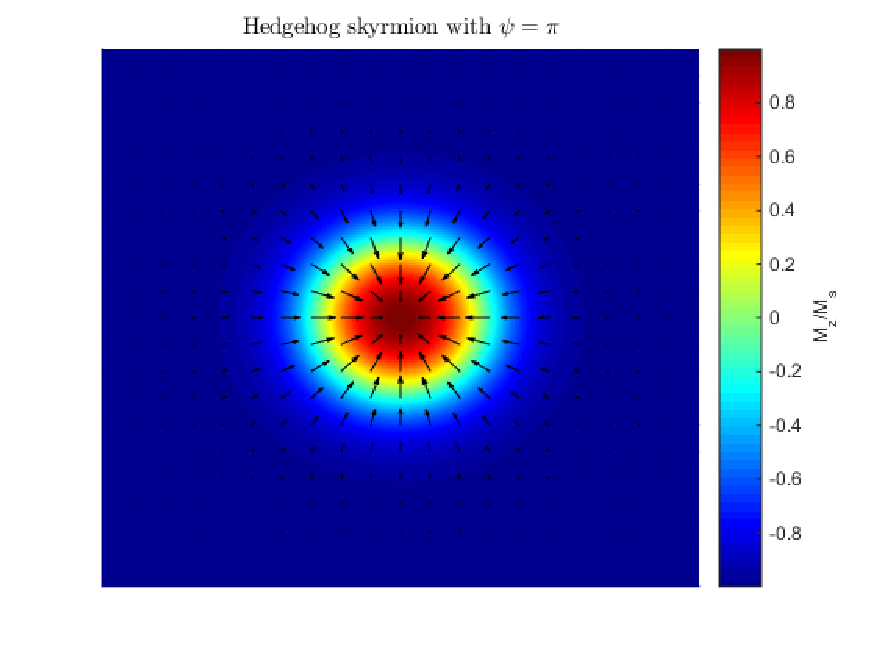
\includegraphics[width=\linewidth]{Figures/HedgehogSkyrmionPsiPi.pdf}
  \caption{}
  \label{fig:HedgehogSkyrmion2}
\end{subfigure}
\newline
\begin{subfigure}{.49\textwidth}
  \centering
  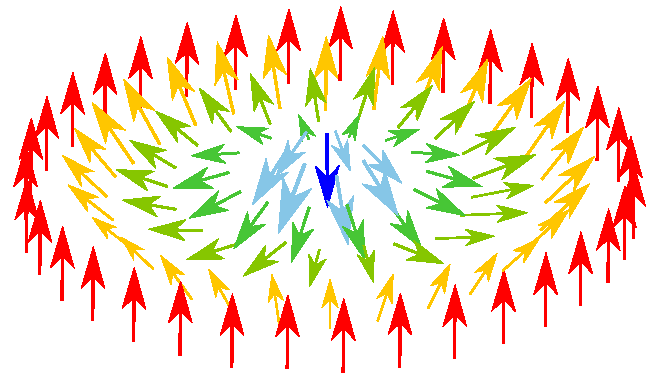
\includegraphics[width=\linewidth]{Figures/HedgehogSkyrmion}
  \caption{}
  \label{fig:HedgehogSkyrmion3}
\end{subfigure}
\caption{A hedgehog skyrmion with a helicity \textbf{(a)} $\psi = 0$ and \textbf{(b)} $\psi = \pi$. The in-plane component of the magnetization is visualized by the vectors, while the $z$-component is shown in the background color. A 3D representation of a hedgehog skyrmion with $\psi = 0$ is shown in \textbf{(c)}, this figure is based on a figure in \cite{EverschorDissertation}.}
\label{fig:HedgehogSkyrmions}
\end{figure}

The results shown so far are based on a system that is stabilized by the interfacial form of DMI. Skyrmions can also be stabilized by the bulk form of DMI, however. Using the ansatz of the skyrmion magnetization profile in \eqref{eq:SkyrmionMVec} in the expression for bulk DMI given by \eqref{eq:DMBulk}, we find the same energy density as for the interfacial DMI $\epsilon_{DM}^{\textrm{(interface)}}$ with the substitution $\cos\psi \rightarrow \sin\psi$. In other words, the skyrmion stabilized by the bulk DMI will have helicities $\psi=\pm\pi/2$, and the $\theta(\rho)$ profile will be the same as for the hedgehog skyrmions stabilized by the interfacial DMI. These types of skyrmions are called spiral skyrmions, as the in-plane magnetization either spirals clockwise or counter-clockwise around the core. From now on we will mostly consider hedgehog skyrmions stabilized by the interfacial form of DMI, as that is the form of DMI that is found in layered thin-film systems that we will study.

\section{Symmetries}
Before moving on to the dynamical properties of the skyrmions we will take a brief interlude to discuss the symmetries of the skyrmion and the LLG equation. This will help us to get further insight into how the different terms in the LLG equation work, and how the skyrmion solutions are related to each other.
\subsection{Time reversal}
Time reversal (or T-symmetry) is a transformation where one reverses the time ($t \rightarrow -t$) as the name indicates. Physical laws that are symmetric under time reversal are reversible processes, while physical laws that break the time reversal symmetry are irreversible processes. Physical variables are either even or odd during time reversal. If they are even they are symmetric under time reversal, and if they are odd they are asymmetric during time reversal. To discuss whether the LLG equation breaks time reversal we need to know how the magnetization $\mathbold{M}$ and the magnetic field $\mathbold{H}$ transform (the constants $\alpha$, $M_s$ and $\gamma$ are all even under time reversal, as they are unrelated to the weak force). It turns out that both $\mathbold{M}$ and $\mathbold{H}$ are odd during time reversal. If we then apply the time reversal transformation to the LLG equation, we end up with
\begin{align}
\label{eq:LLG_TR}
\frac{\textrm{d}\mathbold{M}}{\textrm{d}t} = -\gamma\mathbold{M}\times\mathbold{H}-\frac{\alpha}{M_s}\mathbold{M}\times\frac{\textrm{d}\mathbold{M}}{\textrm{d}t}.
\end{align}
Comparing this to the LLG equation in \eqref{eq:LLG} we see that the LLG equation breaks T-symmetry due to the damping term proportional to $\alpha$. The damping is a dissipative motion, and is therefore an irreversible process. The precession of the magnetization around the magnetic field on the other hand does not break T-symmetry, and is therefore a reversible process.

\subsection{Parity and chirality} \label{sec:Parity}
Parity is a transformation operation which changes the sign of all three cartesian coordinates simultaneously ($\mathbold{r}\rightarrow-\mathbold{r}$), in other words it is a point reflection through the origin. 
%In cylindrical coordinates a parity transformation can be written as $\rho \rightarrow \rho$, $\phi \rightarrow \phi \pm \pi$, $z \rightarrow -z$. Let us now first consider the parity transformation of a magnetic skyrmion. The skyrmion depends on the cylindrical coordinates $\rho$ and $\phi$, as seen from \eqref{eq:SkyrmionMVec}. There is no explicit dependence on $z$, meaning the magnetization pattern is isotropic in the $z$-direction. Since $\rho$ is even under the parity transformation, the entire effect of the operation lies in the change in $\phi$. We remember that the in-plane angle of the magnetization $\Phi$ was given by $\Phi = \phi + \psi$. After a parity transformation this becomes $\Phi = \phi + \psi \pm \pi$. The helicity $\psi$ is a constant, and we can therefore include the change $\pm\pi$ in the helicity of the skyrmion. A magnetic skyrmion has two possible helicities (a hedgehog skyrmion stabilized by interfacial DMI can have $\psi = 0$ or $\psi = \pi$, while a spiral skyrmion stabilized by bulk DMI can have $\psi = \pm\pi/2$) that are a constant $\pi$ apart from each other. A parity transformation then transforms the helicity of the magnetic skyrmion to its other possible value. As a cross-check we also see that two consecutive parity transformations become an identity transformation. In other words, the magnetization pattern of the skyrmion breaks parity. This is a result of the Dzyaloshinskii--Moriya interaction, which is an interaction that violates parity. 
To dicuss parity we first introduce the notion of pseudovectors and pseudoscalars. Normally, vectors are odd under a parity transformation, meaning the transformation changes the sign of the vector, while scalars are even under a parity transformation. Pseudovectors and pseudoscalars behave the opposite way, however. A pseudovector will behave as a vector during a rotation, but during a reflection it behaves differently. An example of a pseudovector is the antisymmetric cross-product between two vectors, which is illustrated in Figure \ref{fig:Parity}. 
\begin{figure}[h!]
\centering
\begin{subfigure}{.43\textwidth}
  \centering
    \begin{tikzpicture}
\node[above right] (img) at (0,0) {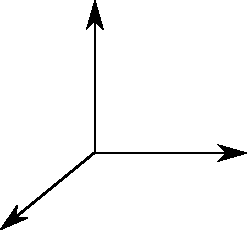
\includegraphics[width=1\textwidth]{Figures/Cartesianv2}};
\node at (40pt,15pt) {\Large{$\mathbold{\hat{x}}$}};
\node at (95pt,175pt) {\Large{$\mathbold{\hat{z}}$}};
\node at (190pt,85pt) {\Large{$\mathbold{\hat{y}}$}};
\end{tikzpicture}
  \caption{}
\end{subfigure}%
\hspace{1cm}
\begin{subfigure}{.33\textwidth}
  \centering
    \begin{tikzpicture}
\node[above right] (img) at (0,0) {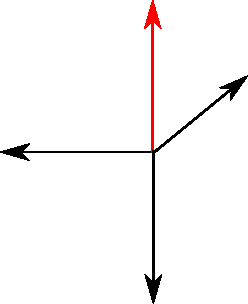
\includegraphics[width=1\textwidth]{Figures/Parityv2}};
\node at (10pt,80pt) {\Large{$\mathbold{\hat{y}}'$}};
\node at (80pt,15pt) {\Large{$\mathbold{\hat{z}}'$}};
\node at (150pt,150pt) {\Large{$\mathbold{\hat{x}}'$}};
\node at (60pt,175pt) {\textcolor{red}{\Large{$\mathbold{\hat{x}}'\times\mathbold{\hat{y}}'$}}};
\end{tikzpicture}
  \caption{}
\end{subfigure}
\caption{An illustration of how cross-products do not transform as vectors under parity. In \textbf{(a)} we see a cartesian coordinate system. Performing a parity transformation on this right-handed coordinate system gives us the left-handed coordinate system in \textbf{(b)}. The pseudovector $\mathbold{\hat{x}}\times\mathbold{\hat{y}}$, which in our right-handed system is equal to $\mathbold{\hat{z}}$, is even under the parity transformation, while the vector $\mathbold{\hat{z}}$ is odd. }
\label{fig:Parity}
\end{figure}
A pseudoscalar is the symmetric dot-product between a pseudovector and a vector. When studying the parity of an expression, the folowing relations may be useful:
\begin{subequations}
\begin{align}
    \label{eq:Pseudovector}
    \textrm{vector}\times\textrm{vector} &= \textrm{pseudovector}, \\
    \label{eq:Vector}
    \textrm{vector}\times\textrm{pseudovector} &= \textrm{vector}, \\
    \label{eq:PseudovectorPseudo}
    \textrm{pseudovector}\times\textrm{pseudovector} &= \textrm{pseudovector}, \\
    \label{eq:Scalar}
    \textrm{vector}\cdot\textrm{vector} &= \textrm{scalar}, \\
    \label{eq:Pseudoscalar}
    \textrm{vector}\cdot\textrm{pseudovector} &= \textrm{pseudoscalar}, \\
    \label{eq:ScalarPseudo}
    \textrm{pseudovector}\cdot\textrm{pseudovector} &= \textrm{scalar}.
\end{align}
\end{subequations}
Now we must consider how the vectors in our equations transform under a parity operation. The relevant vectors are $\mathbold{M}$, $\mathbold{H}$, $\mathbold{E}$, $\mathbold{\nabla}$, $\mathbold{\hat{x}}$, $\mathbold{\hat{y}}$ and $\mathbold{\hat{z}}$. The magnetization and magnetic field are both pseudovectors, and are even under a parity transformation (FIND CITATION). The unit vectors in cartesian coordinates are ordinary vectors, and therefore odd under a parity transformation. As a consequence, the components of the magnetization $M_x$, $M_y$ and $M_z$ are all pseudoscalars, which can be seen from \eqref{eq:Pseudoscalar}. The electric field is also odd under a parity transformation (FIND CITATION), which means that the electric field components behave as scalars, as seen from \eqref{eq:Scalar}. Lastly the $\mathbold{\nabla}$ operator also transforms as a vector, and is therefore odd under parity.

We now have all the results we need to consider the parity of the LLG equation, the effective field, the micromagnetic energy and the skyrmion magnetization. Starting off with the LLG equation \eqref{eq:LLG}, we see that it does not break parity explicitly as long as $\mathbold{H}$ is even under a parity transformation by using the relation in \eqref{eq:PseudovectorPseudo}. When considering the micromagnetic energy terms, all are found to be even under a parity transformation with the exception of the DMI terms (which holds true for both the bulk form of DMI in \eqref{eq:DMBulk} and the interfacial form in \eqref{eq:DMInterface}). At first glance, however, it may seem like the interfacial form of the DMI energy density in \eqref{eq:DMInterface} is even under parity. The reason for this is that while going from the original expression in \eqref{eq:DMIHamiltonian} (which is seen to break parity from \eqref{eq:PseudovectorPseudo} as $\mathbold{D}_{ij}$ is a vector and $\mathbold{S} \propto \mathbold{M}$ is a pseudovector) we have eliminated a cross product. As one can see in \eqref{eq:DMInterfaceCrossP} we have terms that go as $\mathbold{\hat{x}}\cdot(\mathbold{\hat{y}}\times\mathbold{\hat{z}})$ and $\mathbold{\hat{y}}\cdot(\mathbold{\hat{z}}\times\mathbold{\hat{x}})$. In \eqref{eq:DMInterface} these vector expressions are simplified to be unity, which is correct, but hides some of the information when we want to study parity. As $\mathbold{\hat{y}}\times\mathbold{\hat{z}}$ and $\mathbold{\hat{z}}\times\mathbold{\hat{x}}$ are pseudovectors, $\mathbold{\hat{x}}\cdot(\mathbold{\hat{y}}\times\mathbold{\hat{z}})$ and $\mathbold{\hat{y}}\cdot(\mathbold{\hat{z}}\times\mathbold{\hat{x}})$ are in fact pseudoscalars which we can see from \eqref{eq:Pseudoscalar}. So in reality there is a unity pseudoscalar lurking in the expression in \eqref{eq:DMInterface}, making it seem like it is even under parity while in reality it is not. This same pseudoscalar is carried onwards to the DMI term in the effective field in \eqref{eq:EffectiveField}, making part of the effective field odd under parity and thereby violating parity in the LLG equation.

%In summary, it is found that the Dzyaloshinskii--Moriya interaction is the cause of the parity violation in the LLG equation and the skyrmion magnetization pattern, regardless if it is in its bulk or interfacial form.

Moving on to the skyrmion magnetization pattern we use that $\mathbold{M}$ is even under parity, while its components $M_x$, $M_y$ and $M_z$ are not. Remembering that $\mathbold{\hat{M}} = \left(\cos\Phi\sin\theta, \sin\Phi\sin\theta, \cos\theta\right)$ we see that all the components are odd under parity if $\Phi$ transforms as $\Phi \rightarrow \Phi \pm \pi$ and $\theta$ transforms as $\theta\rightarrow\pi-\theta$. This is reminiscent of something we have seen earlier. In Section \ref{sec:Skyrmions} we noted that the solutions for the two different helicities were related by \eqref{eq:ThetaHelicityRelation}, which is the same as the way $\theta$ transforms under parity. In addition the two possible helicities for the different types of skyrmions, hedgehog and spiral, are always a phase $\pm\pi$ apart. The term $\pm\pi$ in the transformation of $\Phi$ under parity can then be included in the helicity, meaning the parity transformation changes the helicity of the skyrmion. The two possible solutions of the skyrmions, such as the hedgehog skyrmions in Figure \ref{fig:HedgehogSkyrmion1} and \ref{fig:HedgehogSkyrmion2}, are therefore related to each other via parity. If the skyrmion in \ref{fig:HedgehogSkyrmion1} is the solution in a right-handed coordinate system, the skyrmion in \ref{fig:HedgehogSkyrmion2} is the same solution in a left-handed coordinate system, and vice versa.
\begin{figure}[h!]
\centering
\begin{subfigure}{.39\textwidth}
  \centering
  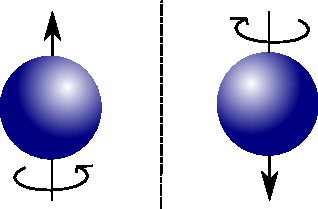
\includegraphics[width=1.0\linewidth]{Figures/UpDownSpinMirror}
  \caption{}
\end{subfigure}%
\hspace{1cm}
\begin{subfigure}{.5\textwidth}
  \centering
  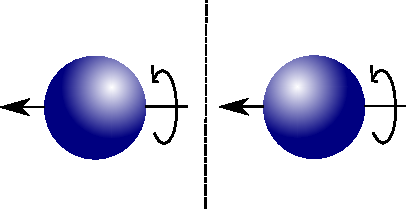
\includegraphics[width=1.0\linewidth]{Figures/LeftSpinMirror}
  \caption{}
\end{subfigure}
\caption{An electron that has a spin vector parallel to a mirror plane will have its spin reversed in its mirror image, as shown in \textbf{(a)}. An electron with a spin perpendicular to the mirror plane, however, will have the same spin as its mirror image as shown in \textbf{(b)}.}
\label{fig:SpinMirror}
\end{figure}
\begin{figure}[h!]
\centering
\begin{subfigure}{.95\textwidth}
  \centering
  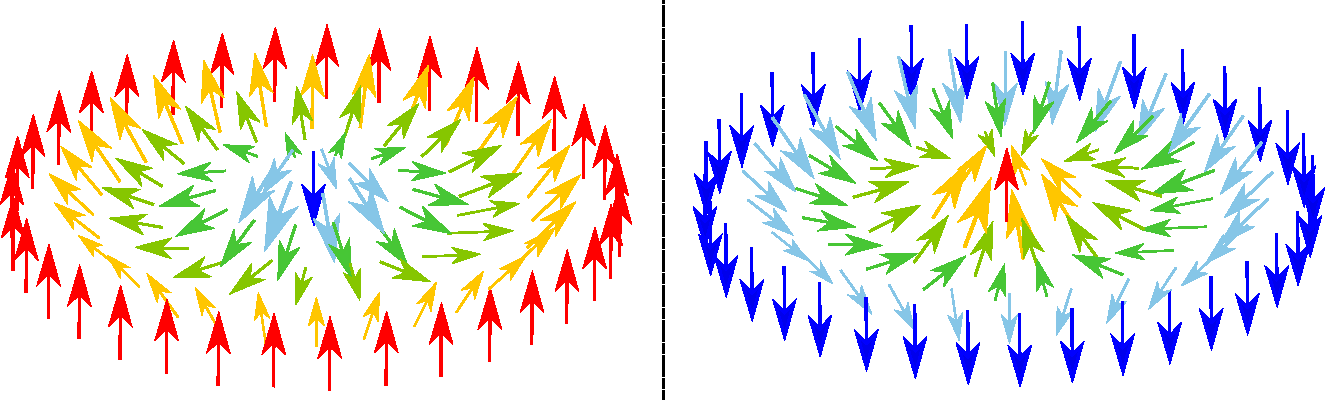
\includegraphics[width=\linewidth]{Figures/MirroredHedgehogSkyrmion.pdf}
  \caption{}
  \label{fig:MirrorHedgehog}
\end{subfigure}

\begin{subfigure}{.95\textwidth}
  \centering
  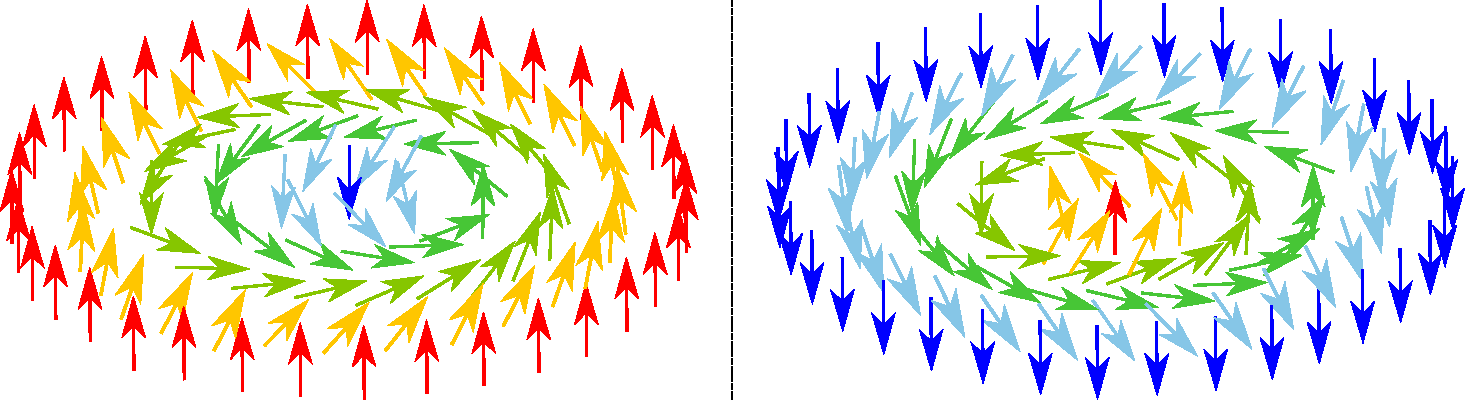
\includegraphics[width=\linewidth]{Figures/MirroredSpiralSkyrmionv2.pdf}
  \caption{}
  \label{fig:MirrorSpiral}
\end{subfigure}
\caption{The mirror images of \textbf{(a)} a hedgehog skyrmion, and \textbf{(b)} a spiral skyrmion. The mirror images can not be aligned with the original image, and the skyrmions are therefore chiral objects. The skyrmion figures are based on the figures in \cite{EverschorDissertation}.}
\label{fig:ChiralitySkyrmions}
\end{figure}

As a final comment on the symmetries of the skyrmions, we want to discuss their chirality. An object is defined to be chiral if its mirror image or reflection is impossible to align with the original object. The most common example of chirality is hands. When holding your right hand in front of a mirror, the image you see in the mirror is that of a left hand. Obviously, a right hand and a left hand are distinct, and can therefore not be aligned with each other. Hands are then chiral objects. When we are considering a mirror image of a skyrmion, we need to be careful regarding what we take the mirror image of. The mirror image of a skyrmion is \textit{not} the mirror image of the skyrmion magnetization vector field. The magnetization of the skyrmion stems from the average magnetic moment inside a small volume, and the magnetic moment is proportional to the spinning of the electron. As we see in Figure \ref{fig:SpinMirror}, when we mirror the spinning motion of the electron the spin vector is not its mirror image. The component of the spin vector parallel to the mirror plane is flipped, while the perpendicular component is the same for both the original electron and its mirror image. This type of behavior occurs for the mirror image of pseudovectors (also known as axial vectors). As the magnetization is also a pseudovector, the mirror images of the skyrmion profiles will behave in the same manner, and are as shown in Figure \ref{fig:ChiralitySkyrmions}. No matter how one rotates the mirror images of the skyrmion magnetization, one can not align them with the original skyrmion. The skyrmions are therefore chiral. This is a consequence of the broken parity of the skyrmion magnetization profile due to the Dzyaloshinskii--Moriya interaction. If the parity transformation of an object is not an identity transformation, it is a chiral object.

\section{The Thiele equation}
In the special case of a time-dependent magnetization pattern that can be written as $\mathbold{M}(\mathbold{r}-\mathbold{R}(t))$, Thiele recognized \cite{Thiele1973} that the time derivative can be written as 
\begin{align}
\label{eq:ThieleRelation}
\frac{\textrm{d} \mathbold{M}}{\textrm{d} t} = \frac{\partial \mathbold{R}}{\partial t}\frac{\partial \mathbold{M}}{\partial \mathbold{R}} = \frac{\partial \mathbold{R}}{\partial t} (-\frac{\partial \mathbold{M}}{\partial \mathbold{r}}) = -(\mathbold{v}\cdot\nabla)\mathbold{M}.
\end{align}
The form $\mathbold{M}(\mathbold{r}-\mathbold{R}(t))$ indicates that the magnetization pattern performs a translation without deformation of the original magnetization profile. Once the equilibrium profile at some time $t_0$ is known, the motion of the entire magnetization pattern can be described by the time-dependent position of some distinct part of the magnetization pattern, like the skyrmion core. If one replaces all time derivatives with Thiele's relation as given above in the LLG equation, one can rewrite the LLG equation to the Thiele equation (as shown by Kr\"{u}ger in \cite{krugerDissertation}):
\begin{align}
\label{eq:Thiele}
\mathbold{F} + \mathbold{G}\times(\mathbold{v}+b_J\mathbold{\hat{j}}_e) + D(\alpha\mathbold{v}+\beta b_J\mathbold{\hat{j}}_e) = 0.
\end{align}
This is a force equation with the definitions
\begin{subequations}
\label{eq:ThieleFGD}
\begin{align}
\label{eq:ThieleF}
\mathbold{F} &= -\frac{\partial E}{\partial \mathbold{R}} = -\mu_0\int \d V\sum_k (\mathbold{\nabla}M_k)(H_k), \\
\label{eq:ThieleG}
\mathbold{G} &= \frac{2\pi M_s\mu_0 d}{\gamma'}\left[\cos\theta\right]_{\theta(r=0)}^{\theta(r=\infty)} \mathbold{\hat{z}},\\
\label{eq:ThieleD}
D &= - \frac{\pi M_s \mu_0 d}{\gamma '} \int_0^{\infty} \d r \left(r\left(\frac{\partial \theta}{\partial r}\right)^2+\frac{\sin^2\theta}{r}\right),
\end{align}
\end{subequations}
where $d$ is the thickness of the film. The vector $\mathbold{F}$ is a force originating from an inhomogenous energy landscape or a magnetic field that is not parallel to the local magnetization (in other words a field not aligned with the effective field). $\mathbold{G}$ is a gyrovector that only depends on the direction of the magnetization in the skyrmion core and far away from the core. The force in the Thiele equation that is dependent on $\mathbold{G}$ is often called the Magnus force, and is a counter force to the Lorentz forces from emergent electromagnetic fields around the skyrmion \cite{Everschor-Sitte2014}, which we will discuss in the next section. Lastly, $D$ denotes the strength of a dissipative force that moves the skyrmion in the direction of the electron flow and it is dependent on the radial profile of the out-of-plane angle $\theta$ of the skyrmion. An illustration of the force balance in the Thiele equation is shown in Figure \ref{fig:Thiele}. The Thiele equation is less rigid than the LLG equation due to the ansatz that there is an absence of deformation of the skyrmion, but in the case of a pure translational motion of the skyrmion the Thiele and LLG equations are entirely equivalent.
\begin{figure}[h!]
\centering
  \centering
    \begin{tikzpicture}
\node[above right] (img) at (0,0) {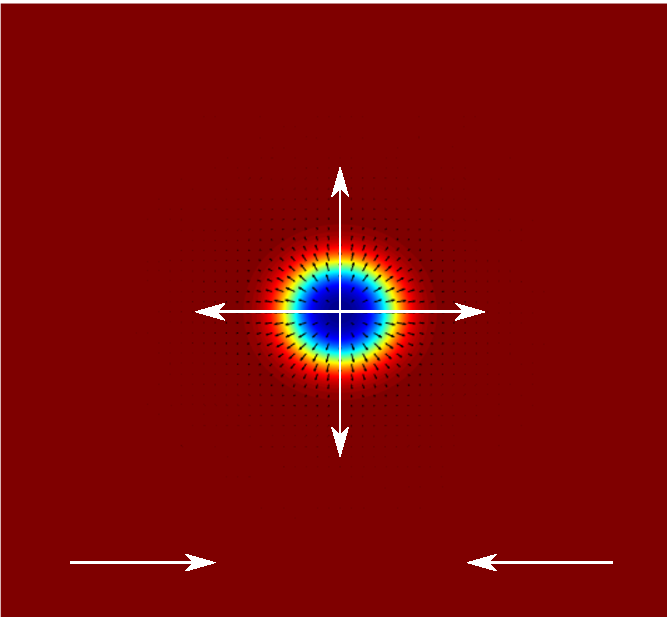
\includegraphics[width=0.6\textwidth]{Figures/SkyrmionThielev2}};
\node at (60pt,40pt) {\textcolor{white}{\Large{$\mathbold{\hat{j}}$}}};
\node at (230pt,40pt) {\textcolor{white}{\Large{$\mathbold{v}$}}};
\node at (50pt,130pt) {\textcolor{white}{\Large{$D\beta b_J\mathbold{\hat{j}}$}}};
\node at (230pt,130pt) {\textcolor{white}{\Large{$D\alpha \mathbold{v}$}}};
\node at (140pt,60pt) {\textcolor{white}{\Large{$\mathbold{G}\times \mathbold{v}$}}};
\node at (147pt,200pt) {\textcolor{white}{\Large{$\mathbold{G}\times b_J\mathbold{\hat{j}}$}}};
\end{tikzpicture}
\caption{An example of the forces in the Thiele equation. In the example shown $\alpha=\beta$ and $\mathbold{v}=-b_J\mathbold{\hat{j}}$. The forces vetors are only there to show direction, and not magnitude. The goal of the Thiele equation is finding a velocity $\mathbold{v}$ that makes all the forces add up to zero.}
\label{fig:Thiele}
\end{figure}

\section{Berry phase, emergent fields, and the topological Hall effect} \label{sec:Berry}
When discussing the dynamics of skyrmions, it will be useful to have some knowledge on Berry phases. The Berry phase \cite{Berry1984}, also known as a geometric phase, is a rotational angle gained by a vector when it undergoes parallel transport on a closed path on a curved surface, as illustrated in Figure \ref{fig:Berry}.
\begin{figure}[h!]
\centering
  \centering
  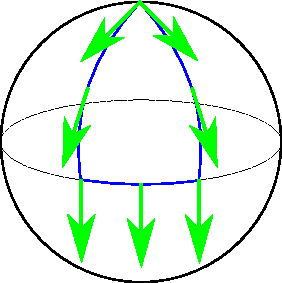
\includegraphics[width=.4\linewidth]{Figures/BerryPhase}
\caption{When a vector undergoes a parallel transport along a closed path on a sphere, it will not be in the same state when arriving back at its starting point. It is rotated with respect to the initial vector, and this rotational angle is known as the Berry phase.}
\label{fig:Berry}
\end{figure}
If the closed path was in a plane, however, the vector will not gain a rotation along its cycle. Skyrmions are magnetization patterns that can be located in a plane, so why is then the Berry phase of interest when electrons move in that plane? When we first started discussing skyrmions, we said that the skyrmion wraps around the unit sphere. In other words, while the magnetization of the skyrmion is located in a plane, the topology of the magnetization pattern behaves in a way so that it can be described as lying on a spherical surface \cite{Everschor-Sitte2014}. 
\begin{figure}[h!]
\centering
\begin{subfigure}{.5\textwidth}
  \centering
  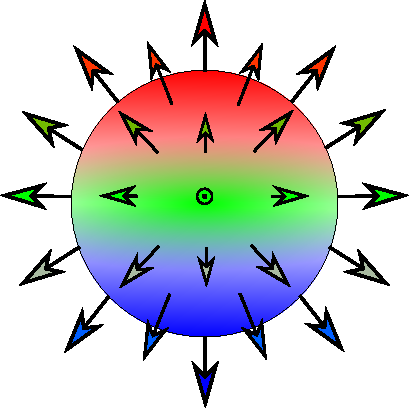
\includegraphics[width=1.0\linewidth]{Figures/HedgehogSphere}
  \caption{}
\end{subfigure}%
\hspace{1cm}
\begin{subfigure}{.35\textwidth}
  \centering
  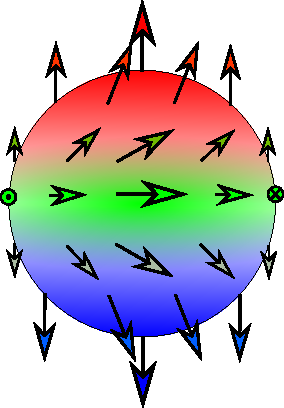
\includegraphics[width=1.0\linewidth]{Figures/SpiralSphere}
  \caption{}
\end{subfigure}
\caption{Skyrmions magnetization patterns mapped onto a spherical surface. The magnetization at $r=0$ is at the bottom of the sphere, while the magnetization at $r=\infty$ is at the top. In \textbf{(a)} we see a hedgehog skyrmion with $\psi = 0$, while in \textbf{(b)} we see a spiral skyrmion with $\psi = \pi/2$.}
\label{fig:SkyrmionSphere}
\end{figure}
This is illustrated in Figure \ref{fig:SkyrmionSphere}. So despite the fact that the conduction electrons from an applied current are moving in a plane, their magnetic moment will still gain a Berry phase when following the magnetization of the skyrmion adiabatically due to the topology of the skyrmion \cite{Tatara2007, Binz2008}. When moving through the skyrmion magnetization, the conduction electrons path is then bent away from the initial direction of the current. This can be seen as a force acting on the conduction electrons, and then there must be an equal force acting in the opposite direction on the skyrmion magnetization. This movement perpendicular to the current direction is known as the topological Hall effect \cite{Ye1999}, as it depends entirely on the topology of the magnetization.

Another way one can look at the cause of the topological Hall effect is the emergent fields approach. Far away from the skyrmion core the magnetization is uniformly pointing in the same direction, while in the vicinity of the skyrmion it has a spatial variation. The spatial variation in the magnetization causes a local variation in the magnetic field that deviates from the uniform field far away from the skyrmion core. The magnetic field can then be written as a superposition of a uniform magnetic field and an emergent magnetic field in the vicinity of the skyrmion, with the components of the emergent magnetic field being given by \cite{Nagaosa2012, Schulz2012}
\begin{align}
    \mathbold{B}_i^e = \frac{\hbar}{2e}\varepsilon_{ijk}\mathbold{\hat{M}}\cdot(\partial_j\mathbold{\hat{M}}\times \partial_k \mathbold{\hat{M}}).
\end{align}
This total magnetic flux from this emergent field is quantized by the skyrmion number $N_{\textrm{sk}}$ given by \eqref{eq:SkyrmionNumber}, which can be seen by integrating the expression above over the skyrmion plane. This magnetic field then causes the conduction electrons to experience a Lorentz force
\begin{align}
    \mathbold{F}_{\textrm{Lorentz}} = q(\mathbold{E} + \mathbold{v}\times\mathbold{B}).
\end{align}
As the emergent magnetic field is spatially varying in the vicinity of the skyrmion, the Lorentz force acting on the conduction electrons around the skyrmion differs from the Lorentz force acting on them far away from the core. If one assumes the skyrmion magnetization to be localized in the $xy$-plane and to be isotropic in the $z$-direction, then the emergent field $\mathbold{B}_i^e$ points along the $z$-axis. This means that the Lorentz force originating from the emergent magnetic field is localized in the $xy$-plane, and is perpendicular to the motion of the conduction electrons. This bending of the electrons' motion can induce a motion of the skyrmion perpendicular to the direction of the current. In addition to the emergent magnetic field, there will also be an emergent electric field once the skyrmion magnetization starts moving, for example due to spin-transfer torques where the magnetic moment of the conduction electrons is transferred to the local magnetization. As seen from the Maxwell--Faraday equation,
\begin{align}
    \nabla\times\mathbold{E} = -\partial_t\mathbold{B},
\end{align}
once the magnetization pattern starts moving the emergent magnetic field will become time dependent, and thereby induce an emergent electric field. This emergent field is given by
\begin{align}
\label{eq:EmergentE}
\mathbold{E}_i^e = \frac{\hbar}{e} \mathbold{\hat{M}}\cdot(\partial_i\mathbold{\hat{M}}\times\partial_t\mathbold{\hat{M}}).
\end{align}
This electric field will also cause the electrons to feel a Lorentz force, and as we can see from the expression above this force is perpendicular to the motion of the skyrmion. Through these emergent fields we can then get an intuitive explanation of the topological Hall effect.

\chapter{Electric control of skyrmion motion} \label{chap:SkyrmionDynamics}
Since it was shown theoretically by Berger \cite{Berger1978,Berger1984,Berger1992,Berger1996} and Slonczewski \cite{Slonczewski1996} that a spin-polarized current could exert a torque on the magnetization in magnetic materials, there has been a lot of focus on electrical control of magnetization dynamics. Through the spin-transfer torque mechanism, one was able to switch the magnetization direction in a magnetic layer solely by applying a current through the material \cite{Myers1999,Sun1999,Katine2000}. This magnetization switching could for example be achieved by a current induced motion of magnetic domain walls \cite{Yamanouchi2004,Yamaguchi2004,Saitoh2004,Yamanouchi2006}. 

It has been shown that skyrmions can also be moved by applying a current, and they can be moved by a much weaker current than magnetic domain walls \cite{Jonietz2010,Yu2012}, which is the reason for the new interest in them. Recently it has also been shown that the motion of skyrmions can also be guided through the means of electric fields \cite{Upadhyaya2015}. It has also been discovered that through the help of constricted geometries and electrical currents, we can create skyrmions in chiral magnets \cite{Iwasaki2013,Sampaio2013,Jiang2015}. In addition we are able to detect skyrmions with an unpolarized current \cite{Monchesky2015}. These new developments will greatly help us in utilizing magnetic skyrmions in memory applications, such as racetracks. 

The goal of this chapter is to study the equations of motion for the skyrmion, both analytically and numerically, so that we can see how we can steer the motion of the skyrmion in the direction we want. We will consider the motion due to an inhomogeneous electric field and an electric current, which will cause the magnetization to experience Rashba fields due to the broken inversion symmetry. An understanding of how we can control the motion of skyrmions by electrical means will be very useful in regards to how we can utilize skyrmions in memory applications.
\section{Skyrmion velocity}
The extended LLG equation that includes Rashba spin-orbit coupling and spin-transfer torques is given by
\begin{align}
\nonumber \frac{\partial \mathbold{M}}{\partial t} &= -\gamma'\mathbold{M}\times(\mathbold{H}_{\text{eff}}+\mathbold{H}_R-\frac{\beta}{M_s} \mathbold{M}\times\mathbold{H}_R) \\
&\hspace{4.5mm}+\frac{\alpha}{M_s}\mathbold{M}\times\frac{\partial\mathbold{M}}{\partial t} + b_J (\mathbold{\hat{j}}_e\cdot\mathbold{\nabla})\mathbold{M} - \frac{\beta b_J}{M_s} \mathbold{M}\times(\mathbold{\hat{j}}_e\cdot\mathbold{\nabla})\mathbold{M}, 
\label{eq:LLG_EC}
\end{align}
with the Rashba field $\mathbold{H}_R$ being given by
\begin{align}
\mathbold{H}_R = \frac{\alpha_R m_e}{\hbar \mu_0\mu_B}b_J (\mathbold{\hat{z}}\times\mathbold{\hat{j}}_e) = C_R b_J (\mathbold{\hat{z}}\times\mathbold{\hat{j}}_e)
\end{align}
and $b_J$ being a characteristic velocity
\begin{align}
    b_J = \frac{1}{1+\beta^2}\frac{\mu_B P j}{e M_s}.
\end{align}
This result was derived by Kim et al. in \cite{Kim2012} in a manner similar to the approach in Section \ref{sec:GeneralSTT}, where the Rashba Hamiltonian \eqref{eq:RashbaH} was included in the derivation with the s-d Hamiltonian. We now want to find this equation in the Thiele formalism, as it then goes from being a partial differential equation to being an algebraic equation in the velocity components. The terms involving the Rashba field $\mathbold{H}_R$ act as a magnetic field in the LLG equation, and we can therefore use the definition of the force from a magnetic field that is not aligned with the effective field in the Thiele equation as given by \eqref{eq:ThieleF}:
\begin{align}
\mathbold{F}_R &= -\mu_0\int \d V\sum_k (\mathbold{\nabla}M_k)\left[\mathbold{H}_R - \frac{\beta}{M_s}\mathbold{M}\times\mathbold{H}_R\right]_k.
\end{align}
This expression is calculated in Appendix \ref{app:F_RashbaThiele} and is found to be
\begin{align}
\mathbold{F}_R = -\mu_0 \pi\beta C_R b_J M_s d \int_0^{\infty} \d r \left(\frac{\partial \theta}{\partial r} r + \sin\theta\cos\theta \right) \mathbold{\hat{x}}
\end{align}
for a hedgehog skyrmion with $\psi = 0$ and $\theta(r=0)=\pi, \theta(r=\infty)=0$. We have assumed that the direction of the current is $\mathbold{\hat{j}}_e = \mathbold{\hat{x}}$. We will only consider these choices for the remainder of this chapter. This is reasonable, as for our particular choice of geometry with thin films (which is necessary to get a significant contribution from the electric field control) hedgehog skyrmions have the lowest energy due to interfacial DMI. We are also free to define the direction along the current to be the $x$-direction.

We now have the force resulting from Rashba spin-orbit coupling, the next step is then to find the force from an inhomogenous electric field. If we consider an electric field with a constant gradient, the field can then be written in cartesian and skyrmion coordinates as
\begin{subequations}
\begin{align}
E(\mathbold{r}) &= E_x x + E_y y \\
&= E_x x_0 + E_y y_0 + E_x r \cos\phi + E_y r \sin\phi,
\end{align}
\end{subequations}
with $\left( x_0,y_0\right)$ indicating the location of the skyrmion core. If we integrate this energy density over the entire film, we then find that the total energy contribution from the electric field becomes
\begin{align}
\nonumber U_{EF} &= \int \d V \epsilon_{EF} \\
\nonumber &= \eta \int_0^d \d z \int_0^{2\pi}\d \phi \int_0^{\infty}\d r\left( E_x x_0 + E_y y_0 + E_x r \cos\phi + E_y r \sin\phi \right) r \sin^2\theta \\
&= 2\pi\eta d\left(E_x x_0 + E_y y_0\right)\int_0^{\infty}\d r r \sin^2\theta.
\end{align}
Remembering that a gradient of the free micromagnetic energy will result in a force in the Thiele equation, as described by \eqref{eq:ThieleF}, we can write the force resulting from the inhomogenous electric field as
\begin{align}
\nonumber\mathbold{F}_E &= -\mathbold{\nabla}U_{EF} \\
&= -2\pi \eta d \left(E_x \mathbold{\hat{x}} + E_y \mathbold{\hat{y}}\right) \int_0^{\infty}\d r r \sin^2\theta.
\end{align}
The final equation in the Thiele formalism for our model can then be written as
\begin{align}
\mathbold{F}_R+\mathbold{F}_E + \mathbold{G} \times\left(\mathbold{v}+b_J\mathbold{\hat{j}}_e\right) + D\left(\alpha\mathbold{v}+\beta b_J \mathbold{\hat{j}}_e\right) = 0,
\end{align}
where we remember the definitions of the gyrovector $\mathbold{G}$ and dissipation factor $D$ to be
\begin{subequations}
\begin{align}
\mathbold{G} &= \frac{2\pi M_s\mu_0 d}{\gamma'}\left[\cos\theta\right]_{\theta(r=0)}^{\theta(r=\infty)} \mathbold{\hat{z}}\\
D &= - \frac{\pi M_s \mu_0 d}{\gamma '} \int_0^{\infty} \d r \left(r\left(\frac{\partial \theta}{\partial r}\right)^2+\frac{\sin^2\theta}{r}\right).
\end{align}
\end{subequations}
If we divide this equation by the length of $\mathbold{G}$, the non-trivial equations we end up with are
\begin{subequations}
\label{eq:EquationsMotionElectricControl}
\begin{align}
- R b_J - C_E E_x - \dot{y}_0 - \alpha_C \dot{x}_0 - \beta_C b_J &= 0, \\
-C_E E_y + \dot{x}_0 + b_J -\alpha_C\dot{y}_0 &= 0,
\end{align}
\end{subequations}
where we have made the following definitions:
\begin{subequations}
\begin{align}
\alpha_C &= \frac{\alpha}{4} \int_0^{\infty} \d r \left(r\left(\frac{\partial \theta}{\partial r}\right)^2+\frac{\sin^2\theta}{r}\right), \\
\beta_C &=\frac{\beta}{4} \int_0^{\infty} \d r \left(r\left(\frac{\partial \theta}{\partial r}\right)^2+\frac{\sin^2\theta}{r}\right), \\
R &= \frac{\gamma'\beta C_R}{4} \int_0^{\infty} \d r \left(\frac{\partial \theta}{\partial r} r + \sin\theta\cos\theta \right), \label{eq:Rconst}\\
C_E &= \frac{\gamma' \eta}{2\mu_0 M_s}\int_0^{\infty}\d r r\sin^2\theta.
\end{align}
\end{subequations}
Solving the equations in \eqref{eq:EquationsMotionElectricControl} for $\dot{x}_0$ and $\dot{y}_0$ one finally ends up with the velocity components of the motion of a skyrmion under the influence of spin-transfer torque, Rashba spin-orbit coupling and an inhomogenous electric field:
\begin{subequations}
\label{eq:ElectricalSkyrmionVComponents}
\begin{align}
\dot{x}_0 &= - \frac{1+\alpha_C(\beta_C + R)}{\alpha_C^2+1}b_J + \frac{C_E}{\alpha_C^2+1}E_y - \frac{\alpha_C C_E}{\alpha_C^2+1}E_x, \\
\dot{y}_0 &= \frac{\alpha_C-(\beta_C + R)}{\alpha_C^2+1}b_J - \frac{C_E}{\alpha_C^2+1}E_x - \frac{\alpha_C C_E}{\alpha_C^2+1}E_y.
\end{align}
\end{subequations}
From this result we can see the effects of RSOC and an electric field gradient on the velocity of the skyrmion center of mass. The RSOC has the same impact on the motion as the non-adiabatic STT, and appears as a correction to $\beta_C$ in the equations of motion. Note that only the term proportional to $\beta\mathbold{M}\times\mathbold{H}_R$ has an impact on the skyrmion dynamics, as a constant magnetic field like $\mathbold{H}$ can not induce a rigid motion of the skyrmion because there is no energy gain for it to move elsewhere. The constant field $\mathbold{H}_R$ can, however, induce a deformation of the skyrmion. For example, a constant external magnetic field pointing along the $z$-direction perpendicular to the skyrmion plane has an effect on the skyrmion size, much like magnetic anisotropy. If this external field is alternating, the field can cause the skyrmion size to shrink and increase periodically \cite{Mochizuki2012}, and in nanodots it can even be used to switch the magnetization of the core \cite{Zhang2015}. In our case the magnetic field experienced due to the Rashba effect lies in the skyrmion plane, and one would therefore expect it to have other deformation modes than a field pointing perpendicular to the skyrmion plane. To understand the effect of the non-uniform Rashba field proportional to $\beta\mathbold{M}\times\mathbold{H}_R$ we can compare it to the adiabatic STT in \eqref{eq:STT_Adiabatic_Macro}. The term in the LLG equation can be written as $\gamma\beta\mathbold{M}\times(\mathbold{M}\times\mathbold{H}_R)/M_s = -(\gamma\beta C_R b_J/M_s)\mathbold{M}\times(\mathbold{\hat{H}}_R\times\mathbold{M})$. This is very similar to the adiabatic STT acting on a magnetization $\mathbold{M}_j$ from a current that was polarized by passing through a magnetization $\mathbold{M}_i$. This torque was proportional to $-\mathbold{M}_j\times(\mathbold{M}_i\times\mathbold{M}_j)$. With the exception of the different torque magnitudes, the only difference is that the polarizing magnetic layer $\mathbold{M}_i$ is replaced by the Rashba field $\mathbold{H}_R$. This torque then originates from the conduction electrons that are polarized in the direction of the Rashba field. The direction of this field is given by $\mathbold{\hat{H}}_R=\mathbold{\hat{z}}\times\mathbold{\hat{j}}_e$. When the current is passing in the $x$-direction as we have considered so far, this field points in the $y$-direction. As this is generates a component of the spin polarization of the current that can be perpendicular to the local magnetization, it would explain why the torque behaves as the non-adiabatic STT. We now compare the driving torque resulting from RSOC more closely to the non-adiabatic STT. The driving torque from RSOC can be written as
\begin{align}
    \nonumber \gamma\beta\mathbold{m}\times\left(\mathbold{M}\times\mathbold{H}_R\right) &= \gamma\beta M_s\left(\left(\mathbold{m}\cdot\mathbold{H}_R\right)\mathbold{m}-\mathbold{H}_R\right) \\
    &=     
    \gamma\beta M_s C_R b_J
    \begin{pmatrix}
     \sin^2\theta\sin\Phi\cos\Phi \\
     \sin^2\theta\sin^2\Phi-1 \\
     \sin\theta\cos\theta\sin\Phi
    \end{pmatrix},
\end{align}
while the non-adiabatic STT can be written as 
\begin{align}
    -\beta b_J\mathbold{m}\times\left(\mathbold{\hat{j}}_e\cdot\mathbold{\nabla}\right)\mathbold{M} =     
    -\beta b_J M_s
    \begin{pmatrix}
     -\sin\Phi\cos\phi\partial_r\theta + \sin\theta\cos\theta\cos\Phi\sin\phi/r \\
     \cos\Phi\cos\phi\partial_r\theta + \sin\theta\cos\theta\sin\Phi\sin\phi/r \\
     -\sin^2\theta\sin\phi/r
    \end{pmatrix},
\end{align}
where we have used that $\partial_x\theta = -\sin\phi/r\partial_r\theta$ and $\partial_x\Phi = -\sin\phi/r$. If we integrate over the skyrmion plane, the only non-vanishing components in both torques in the $\psi=0$ case ($\Phi=\phi$) is the $y$-component. In addition, we see by performing this integration that we get the integral appearing in the RSOC term in \eqref{eq:Rconst}.

The electric field gradient introduces new terms to the velocity of the skyrmion. We can see that the skyrmion tends to move in a direction perpendicular to the electric field gradient, along $\mathbold{\hat{z}}\times(-\nabla E)$. In addition to the motion perpendicular to the gradient, the Gilbert damping also causes a damped motion in the opposite direction of the field gradient, moving the skyrmion to a lower energy state. The damped motion is relatively easy to understand, as it is nothing else than a relaxation of the magnetization to a lower energy. The motion of the skyrmion along the equipotential lines is a bit less intuitive, however. The reason for this motion is the Magnus force, resulting from the topology of the skyrmion. Initially the skyrmion experiences a force against the electric field gradient. At this point this is the only force acting on the skyrmion, as the Magnus force is only existent when the skyrmion moves. The skyrmion therefore drifts down to a lower energy state to begin with. However, as the the skyrmion starts to move the Magnus force kicks in, as the motion of the skyrmion induces an emergent electric field perpendicular to its motion, as described in Section \ref{sec:Berry}. This new force changes the direction of the skyrmion motion, until the motion is such that the Magnus force and the force from the inhomogeneous energy landscape cancel out, as illustrated in Figure \ref{fig:SkyrmionPotentialLineMotion}. The resulting motion is a Hall-like motion along the equipotential lines. This behaviour that we see from the electric field is analogous to the motion a skyrmion would have in the presence of an electric field in multiferroic insulators \cite{Liu2013}. The mechanism behind the motion due to the electric field is different, however. In multiferroic insulators the electric field couples to the dipole moment of the skyrmion, while in this ferromagnetic metal the motion is caused by a shift in the energy landscape due to the modification of the anisotropic energy by the voltage induced magnetic anisotropy. 

\begin{figure}[h!]
\centering
  \centering
  \begin{tikzpicture}
\node[above right] (img) at (0,0) {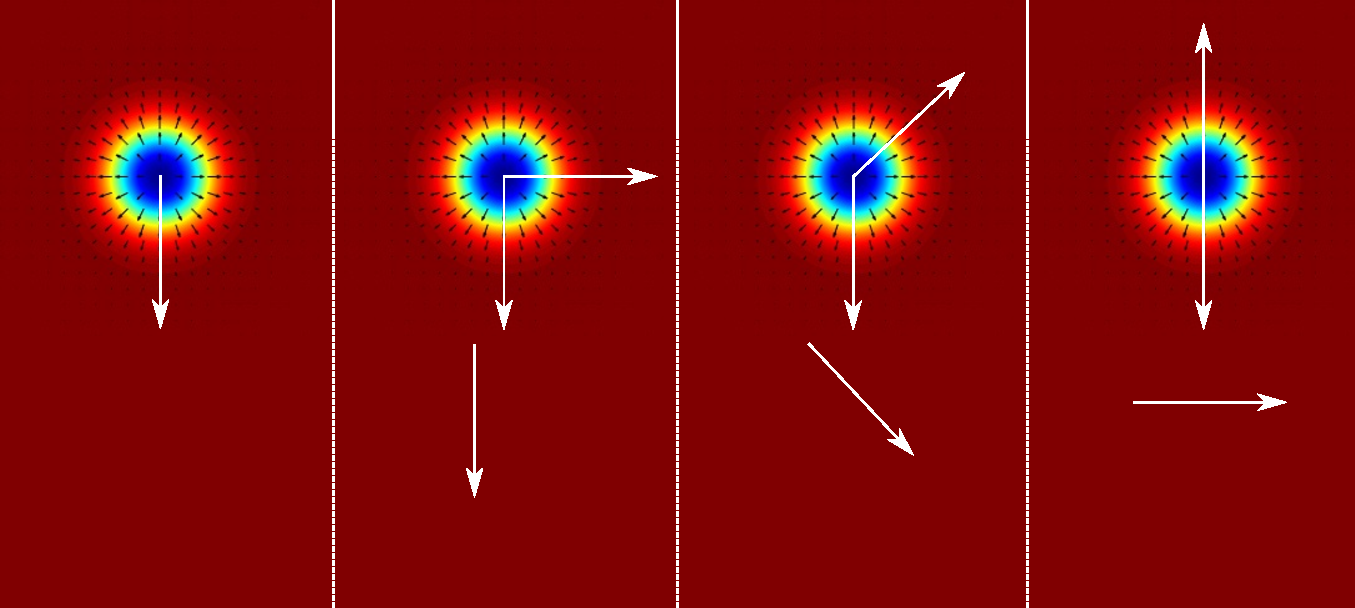
\includegraphics[width=1\textwidth]{Figures/SkyrmionPotentialLineMotionv2}};
\node at (60pt,15pt) {\textcolor{white}{\Large{$t = t_0$}}};
\node at (177pt,15pt) {\textcolor{white}{\Large{$t = t_1$}}};
\node at (294pt,15pt) {\textcolor{white}{\Large{$t = t_2$}}};
\node at (411pt,15pt) {\textcolor{white}{\Large{$t = t_3$}}};
\node at (40pt,120pt) {\textcolor{white}{\Large{$\mathbold{F}_E$}}};
\node at (155pt,120pt) {\textcolor{white}{\Large{$\mathbold{F}_E$}}};
\node at (270pt,120pt) {\textcolor{white}{\Large{$\mathbold{F}_E$}}};
\node at (385pt,120pt) {\textcolor{white}{\Large{$\mathbold{F}_E$}}};
\node at (60pt,60pt) {\textcolor{white}{\Large{$\mathbold{v}=0$}}};
\node at (175pt,60pt) {\textcolor{white}{\Large{$\mathbold{v}$}}};
\node at (290pt,60pt) {\textcolor{white}{\Large{$\mathbold{v}$}}};
\node at (405pt,60pt) {\textcolor{white}{\Large{$\mathbold{v}$}}};
\node at (200pt,180pt) {\textcolor{white}{\Large{$\mathbold{G}\times\mathbold{v}$}}};
\node at (290pt,180pt) {\textcolor{white}{\Large{$\mathbold{G}\times\mathbold{v}$}}};
\node at (380pt,180pt) {\textcolor{white}{\Large{$\mathbold{G}\times\mathbold{v}$}}};
\end{tikzpicture}
\caption{The initial motion due to the force from the spatially varying electric field is redirected due to the appearance of the Magnus force when the skyrmion starts to move. In equilibrium we have a Hall-like motion along the equipotential lines in the absence of Gilbert damping.}
\label{fig:SkyrmionPotentialLineMotion}
\end{figure}

\section{Numerical integrals}
The solution of the skyrmion velocity depends on parameters that are functions of three different integrals. These integrals depend on the solution of $\theta(r)$ that is obtained numerically by solving \eqref{eq:ODEtheta}. As our solution of $\theta$ is a numerical function, the integrals have to be calculated numerically as well. In \eqref{eq:ODEtheta} the only variable parameter is the skyrmion parameter $C = AK/D^2$, so the integrals can be expressed as functions of $C$ and for some of the integrals a dimensional scaling factor. The three integrals that we need to evaluate are
\begin{subequations}
\begin{align}
I_1 &= \int_0^{\infty} \textrm{d} \tilde{r} \left(\tilde{r}\left(\frac{\partial \theta}{\partial \tilde{r}}\right)^2+\frac{\sin^2\theta}{\tilde{r}}\right), \\
I_2 &= \frac{A}{D} \int_0^{\infty} \textrm{d} \tilde{r} \left(\frac{\partial \theta}{\partial \tilde{r}} \tilde{r} + \sin\theta\cos\theta \right), \\
I_3 &= \frac{A^2}{D^2}\int_0^{\infty} \textrm{d} \tilde{r} \tilde{r}\sin^2\theta.
\end{align}
\end{subequations}
Here the solution of $\theta$ inside the integrals is given in the dimensionless length scale $\tilde{r} = r\cdot D/A$. The resulting integrals as functions of $C$ are shown in Figure \ref{fig:ThetaInts}.
\begin{figure}[h!]
\centering
\begin{subfigure}{.49\textwidth}
  \centering
  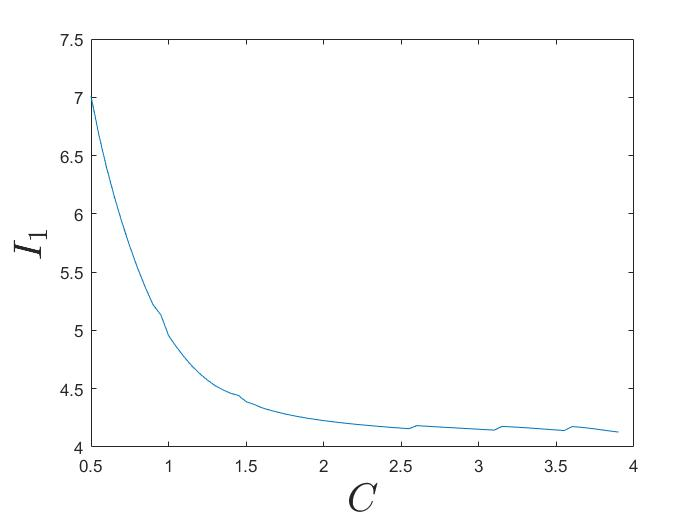
\includegraphics[width=\linewidth]{Figures/I1Plot.jpg}
  \caption{}
  \label{fig:ThetaInt1}
\end{subfigure}
\begin{subfigure}{.49\textwidth}
  \centering
  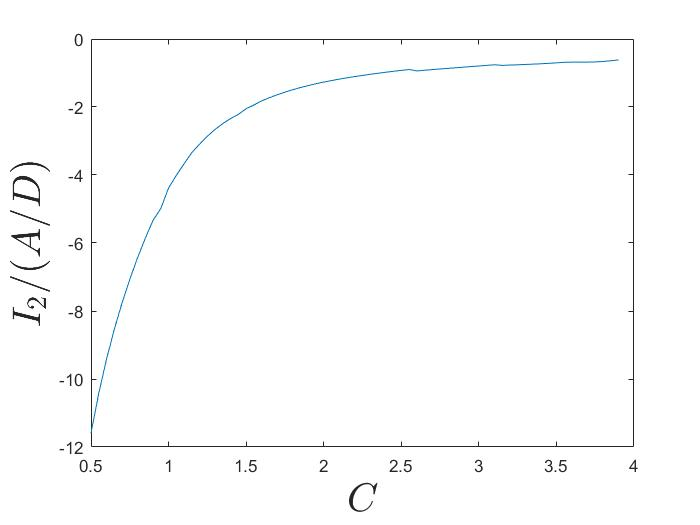
\includegraphics[width=\linewidth]{Figures/I2Plot.jpg}
  \caption{}
  \label{fig:ThetaInt2}
\end{subfigure}
\linebreak
\begin{subfigure}{.49\textwidth}
  \centering
  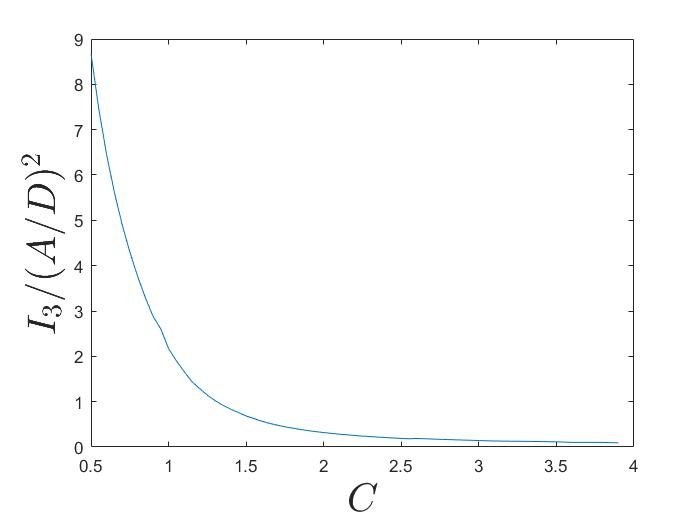
\includegraphics[width=\linewidth]{Figures/I3Plot.jpg}
  \caption{}
  \label{fig:ThetaInt3}
\end{subfigure}
\caption{Numerical evaluations of the integrals \textbf{(a)} $I_1$, \textbf{(b)} $I_2$ and \textbf{(c)} $I_3$ as a function of the skyrmion parameter $C$.}
\label{fig:ThetaInts}
\end{figure}

\section{Pinning, threshold currents and field gradients}
As with domain walls, there is also a threshold current or field that is necessary for skyrmions to start moving, even though our previous results do not reflect this. In the case of skyrmions this threshold current is much weaker than the case of domain walls \cite{Jonietz2010}. The reason for this reluctance to move is pinning centers, which have much less impact on the motion of skyrmions than that of domain walls, but have an impact nonetheless. To model the effect of pinning centers on skyrmion motions at low current densities or weak electric fields, one can introduce a pinning force in the Thiele equation \eqref{eq:Thiele}. The equation of interest then becomes
\begin{align}
\label{eq:PinningThiele}
\mathbold{F}_{\textrm{pin}}+\mathbold{F}_R+\mathbold{F}_E + \mathbold{G} \times\left(\mathbold{v}+b_J\mathbold{\hat{j}}_e\right) + D\left(\alpha\mathbold{v}+\beta b_J \mathbold{\hat{j}}_e\right) = 0.
\end{align}
The phenemenological pinning force $\mathbold{F}_{\textrm{pin}}$ is usually written as \cite{Everschor2012, IwasakiNagaosa2013}.
\begin{align}
\mathbold{F}_{\textrm{pin}} = -4\pi v_{\textrm{pin}} f(\frac{v}{v_{\textrm{pin}}}) \frac{\mathbold{v}}{v},
\end{align}
where the function $f(\frac{v}{v_{\textrm{pin}}})$ goes towards unity for small skyrmion velocities $v$. This is to ensure that the force does not vanish as $v\rightarrow 0$, but there is a constant force barrier that the skyrmion needs to overcome to have a velocity greater than zero. In the low velocity limit one therefore approximates the pinning force by
\begin{align}
\mathbold{F}_{\textrm{pin}} = - v_{\textrm{pin}} \frac{\mathbold{v}}{v},
\end{align}
where the forces are normalized in a way so that the gyrovector $\mathbold{G} = (0, 0, 1)$. The non-trivial equations we then get from \eqref{eq:PinningThiele} are
\begin{subequations}
\label{eq:PinningThieleComponents}
\begin{align}
\label{eq:PinningThieleA}
-\dot{y}_0 - \beta_Cb_J - \alpha_C\dot{x}_0 - v_{\textrm{pin}}\frac{\dot{x}_0}{v} + F_x &= 0, \\
\label{eq:PinningThieleB}
b_J + \dot{x}_0 - \alpha_C\dot{y}_0 - v_{\textrm{pin}}\frac{\dot{y}_0}{v} + F_y &= 0,
\end{align}
\end{subequations}
where $F_x$ and $F_y$ are the $x-$ and $y-$ components of the total force $\mathbold{F}_R + \mathbold{F}_E$ resulting from Rashba spin-orbit coupling and voltage induced magnetic anisotropy respectively. In the case of $F_x = F_y = 0$, one can see that if one makes the substitution
\begin{align}
\alpha_C \rightarrow \alpha_C+\frac{v_{\textrm{pin}}}{v}
\end{align}
the equations of motion are exactly the same as for the case of the motion of a skyrmion due to a spin-polarized current. The solutions of $\dot{x}_0$ and $\dot{y}_0$ are known in this case, and one can therefore make the substitution of $\alpha_C$ above into these solutions to get the solutions in the presence of pinning:
\begin{subequations}
\begin{align}
\dot{x}_0 &= -\frac{1+(\alpha_C+\frac{v_{\textrm{pin}}}{v})\beta_C}{(\alpha_C+\frac{v_{\textrm{pin}}}{v})^2+1}b_J, \\
\dot{y}_0 &= \frac{(\alpha_C+\frac{v_{\textrm{pin}}}{v}) - \beta_C}{(\alpha_C+\frac{v_{\textrm{pin}}}{v})^2+1}b_J.
\end{align}
\end{subequations}
As one can see, these solutions depend on the total skyrmion velocity $v$. To determine this velocity we use the relation $v^2 = \dot{x}_0^2+\dot{y}_0^2$ and the solutions above, which gives us the equation
\begin{align}
v^2 = \frac{\beta_C^2+1}{(\alpha_C+\frac{v_{\textrm{pin}}}{v})^2+1}b_J^2.
\end{align}
Rearranging this equation one can get the following second order equation in $v$:
\begin{align}
(\alpha_C^2+1)v^2+(2\alpha_Cv_{\textrm{pin}})v + (v_{\textrm{pin}}^2-(\beta_C^2+1)b_J^2) = 0.
\end{align}
The solution to this equation is given by
\begin{align}
v = \frac{\sqrt{(\alpha_Cv_{\textrm{pin}})^2+(\alpha_C^2+1)\left[(\beta_C^2+1)b_J^2-v_{\textrm{pin}}^2\right]}-\alpha_Cv_{\textrm{pin}}}{\alpha_C^2+1},
\end{align}
where the positive solution has been chosen as that is the only solution that can give a positive $v$. This solution in $v$ differs from the solution given by Iwasaki et al. \cite{IwasakiNagaosa2013} by the term outside of the square root, but the solutions of $\dot{x}_0$ and $\dot{y}_0$ are in agreement. As our solution of $v$ is consistent with our solutions of $\dot{x}_0$ and $\dot{y}_0$, and if one plugs our solutions into the equations in \eqref{eq:PinningThieleComponents} they are satisfied in the case $F_x = F_y = 0$, it is concluded that our solutions are correct. 

So far we have only discussed pinning of the spin-polarized current driven skyrmion motion, but it is also of interest to find the same results in the presence of Rashba spin-orbit coupling and an imhomogenous electric field perpendicular to the film. In other words, we must solve \eqref{eq:PinningThieleComponents} when $F_x \neq 0$ and $F_y \neq 0$. We apply the same trick again where we try to incorporate $F_x$ and $F_y$ into similar variables in the equations we already have a solution for. $F_x$ and $F_y$ are both independent of $\dot{x}_0$, $\dot{y}_0$ and $v$, we must therefore try to include them in other terms also independent of these variables. In \eqref{eq:PinningThieleA} the only term independent of these is $-\beta_Cb_J$, and in \eqref{eq:PinningThieleB} the term is $b_J$. If we define new variables $\tilde{\beta}_C$ and $\tilde{b}_J$ that satisfy
\begin{subequations}
\begin{align}
-\tilde{\beta}_C\tilde{b}_J &= -\beta_Cb_J + F_x, \\
\tilde{b}_J &= b_J + F_y,
\end{align}
\end{subequations}
meaning they have the following definitions:
\begin{subequations}
\begin{align}
\tilde{\beta}_C &= \frac{\beta_Cb_J-F_x}{b_J+F_y}, \\
\tilde{b}_J &= b_J + F_y,
\end{align}
\end{subequations}
the equations have the same form as before with $\beta_C \rightarrow \tilde{\beta}_C$ and $b_J \rightarrow \tilde{b}_J$. The total force components resulting from $\mathbold{F}_R+\mathbold{F}_E$ are
\begin{subequations}
\begin{align}
F_x &= -C_E E_x - Rb_J, \\
F_y &= -C_E E_y.
\end{align}
\end{subequations}
If we plug these into $\tilde{\beta}_C$ and $\tilde{b}_J$ and make the substitutions in our previous solutions of $\dot{x}_0$, $\dot{y}_0$ and $v$ from the current driven case, we end up with the solutions
\begin{subequations}
\begin{align}
\dot{x}_0 &= -\frac{1+(\alpha_C+\frac{v_{\textrm{pin}}}{v})(\beta_C+R)}{(\alpha_C+\frac{v_{\textrm{pin}}}{v})^2+1}b_J + \frac{C_E}{(\alpha_C+\frac{v_{\textrm{pin}}}{v})^2+1}E_y - \frac{(\alpha_C+\frac{v_{\textrm{pin}}}{v})C_E}{(\alpha_C+\frac{v_{\textrm{pin}}}{v})^2+1}E_x, \\
\dot{y}_0 &= \frac{(\alpha_C+\frac{v_{\textrm{pin}}}{v})-\beta_C - R}{(\alpha_C+\frac{v_{\textrm{pin}}}{v})^2+1}b_J - \frac{C_E}{(\alpha_C+\frac{v_{\textrm{pin}}}{v})^2+1}E_x - \frac{(\alpha_C+\frac{v_{\textrm{pin}}}{v}) C_E}{(\alpha_C+\frac{v_{\textrm{pin}}}{v})^2+1}E_y, \\
\label{eq:PinningVElectrical}
v &= \frac{\sqrt{(\alpha_Cv_{\textrm{pin}})^2+(\alpha_C^2+1)\left[(\beta_Cb_J+Rb_J+
C_EE_x)^2+(b_J-C_EE_y)^2-v_{\textrm{pin}}^2\right]}-\alpha_Cv_{\textrm{pin}}}{\alpha_C^2+1}.
\end{align}
\end{subequations}
It can be seen that in the limit of no pinning ($v_{\textrm{pin}} \rightarrow 0$) the results for $\dot{x}_0$ and $\dot{y}_0$ are in agreement with \eqref{eq:ElectricalSkyrmionVComponents}. From the expression for $v$ in \eqref{eq:PinningVElectrical} it is also possible to determine the threshold current or electric field gradient necessary for the solution of $v$ to be greater than zero. If we first consider the case where the skyrmion motion is solely driven by a spin-polarized current, one finds that the skyrmion moves when $b_J > b_J^{\textrm{(crit)}}$ with
\begin{align}
b_J^{\textrm{(crit)}} = \frac{1}{1+\beta^2} \frac{\mu_BP}{eM_s}j_e^{\textrm{(crit)}}= \frac{v_{\textrm{pin}}}{\sqrt{(\beta_C+R)^2+1}}.
\end{align}
In the field driven case where the skyrmion motion is solely driven by an inhomogenous electric field applied perpendicular to the film, one finds that the skyrmion moves when the field gradient $E_g = \sqrt{E_x^2+E_y^2}$ is greater than some critical value
\begin{align}
E_g^{\textrm{(crit)}} = \frac{v_{\textrm{pin}}}{C_E}.
\end{align}
The numerical values of $b_J^{\text{(crit)}}$ and $E_g^{\text{(crit)}}$ for different values of the skyrmion parameter $C$ are shown in Figure \ref{fig:CritCurrentField}. As one can see, the behavior of the critical current and field gradient are quite different. The critical current is a strictly decreasing function of $C$, but the decrease is only significant for high values of $\beta$. The critical field gradient, however, is a strictly increasing function of $C$, and increases significantly from $C = 0.5$ to $C = 2.5$. If the unit length $A/D$ is kept constant, the size of the skyrmion decreases with increasing $C$ (which can be seen from Figure \ref{fig:ThetaProfile}). Still assuming that $A/D$ is kept constant, one sees that in the current driven case smaller skyrmions have a lower critical current, while in the electric field driven case larger skyrmions have a lower critical field gradient. This can be understood rather intuitively. The non-adiabatic spin-transfer torque acts as a drag force on the skyrmion in the Thiele equation. This drag force attempts to move the skyrmion in the direction of the conduction electrons. Normally the total non-adiabatic STT is larger for larger skyrmions, but with the presence of RSOC we get an effectively reduced non-adiabatic STT. This reduction is greater for larger skyrmions due to the larger area where the conduction electrons polarized along the Rashba field can transfer their spin to the local magnetization. Because of this effective reduction of the non-adiabatic STT larger skyrmions experience less drag along the motion of the conduction electrons, and smaller skyrmions then require a smaller current to be moved than large ones. If RSOC was not present the situation would be reversed, as there is no reduction of the drag resulting from non-adiabatic STT, and larger skyrmions would have a lower critical current due to the larger drag force acting on them. For the electric field driven case the spatial variation of the free energy has a larger impact on a large skyrmion than a small skyrmion.

\begin{figure}[h!]
\centering
\begin{subfigure}{.49\textwidth}
  \centering
  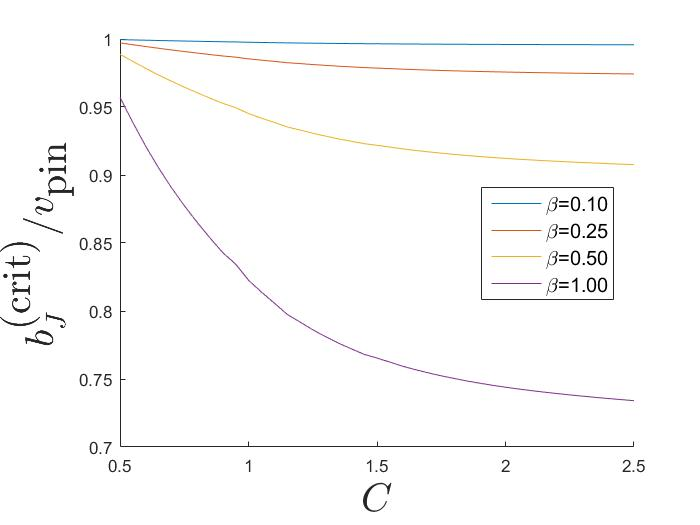
\includegraphics[width=\linewidth]{Figures/CritCurrent.jpg}
  \caption{}
  \label{fig:CritCurrent}
\end{subfigure}
\begin{subfigure}{.49\textwidth}
  \centering
  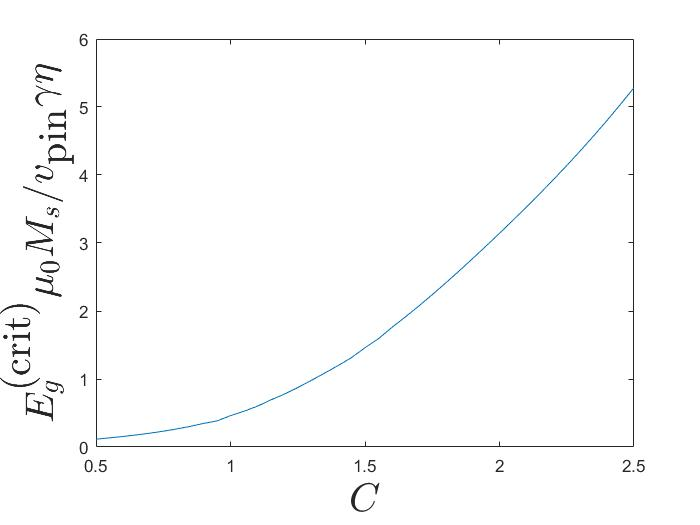
\includegraphics[width=\linewidth]{Figures/CritField.jpg}
  \caption{}
  \label{fig:CritField}
\end{subfigure}
\caption{\textbf{(a)} The critical current density and \textbf{(b)} the critical field gradient as a function of the skyrmion parameter $C$.}
\label{fig:CritCurrentField}
\end{figure}

\section{Numerical simulations}
In our analytical calculations in the previous sections we have solved the Thiele equation, which is a simplification of the LLG equation. The Thiele equation assumes that we have a rigid motion of the skyrmion, so that the motion of the skyrmion can be described by the motion of a key feature of the magnetization pattern such as the skyrmion core. Because of this, the Thiele equation can not describe whether the skyrmion becomes deformed during its motion or not. In some of the cases we have considered so far it is likely that there will at least be certain deformation of the skyrmion profile. The presence of RSOC and application of an electric field gradient to the system will cause the magnetization to experience magnetic fields that are not aligned with the effective field that stabilizes the skyrmion. To judge if our analytical results have any merit, we therefore solve the LLG equation numerically where we make no assumptions regarding the rigidness of the skyrmion motion. We can then compare our analytical results in the Thiele framework with the numerical results in the LLG framework to see if a rigid motion is a good approximation or not.
\subsection{The LLG equation as a parabolic equation}
The LLG equation is a partial differential equation that is first order in time, and contains first and second order spatial derivatives through the effective field from DMI and the exchange interaction in the skyrmion case. It should then be possible to write the LLG equation on the following form:
\begin{align}
\label{eq:LLG_PDE}
\bar{d}\mathbold{\dot{m}} - \nabla\cdot(\mathbold{\bar{c}}\otimes\nabla \mathbold{m}) + \bar{a}\mathbold{m} = \mathbold{f}.
\end{align}
Here $\mathbold{m}$ and $\mathbold{f}$ are vectors of length $N$, $\bar{d}$ and $\bar{a}$ are $N\times N$ matrices, and $\mathbold{\bar{c}}$ is a $N_{\textrm{dim}}\times N_{\textrm{dim}} \times N\times N$ tensor. For the case of the skyrmion, we have three magnetization components we need to solve for in a 2D plane, in other words $N = 3$ and $N_{\textrm{dim}}=2$. Equations on the form given by \eqref{eq:LLG_PDE} are solved by the \texttt{parabolic} function in \texttt{MATLAB}'s \texttt{PDE Toolbox}, which utilizes a finite element method. We then need to rewrite \eqref{eq:LLG_EC} to the form of \eqref{eq:LLG_PDE}. This was done and provided the following results:
\begin{subequations}
\begin{align}
\mathbold{f} &= 
 \begin{pmatrix}
  b_J\partial_x m_x - \beta b_J(m_y\partial_xm_z - m_z\partial_xm_y) + 2(m_y\partial_xm_x+m_y\partial_ym_y+m_z\partial_ym_z)\gamma D/(\mu_0M_s)\\
  b_J\partial_x m_y - \beta b_J(m_z\partial_xm_x-m_x\partial_xm_z)-2(m_z\partial_xm_z+m_x\partial_xm_x+m_x\partial_ym_y) \gamma D/(\mu_0M_s) -\beta H_R\\
  b_J\partial_xm_z - \beta b_J(m_x\partial_xm_y-m_y\partial_xm_x) - 2(m_x\partial_ym_z-m_y\partial_xm_z)\gamma D/(\mu_0M_s)
 \end{pmatrix}, \\
\bar{d} &= 
 \begin{pmatrix}
  1 & \alpha m_z & -\alpha m_y \\
  -\alpha m_z & 1 & \alpha m_x \\
  \alpha m_y & -\alpha m_x  & 1
 \end{pmatrix}, \\
 \bar{a} &= 
 \begin{pmatrix}
  -\gamma \beta H_R m_y & 2\gamma (K+\eta E) m_z/(\mu_0M_s) & -\gamma H_R \\
  -2\gamma (K+\eta E) m_z/(\mu_0M_s) & -\gamma\beta H_R m_y & 0 \\
  \gamma H_R & 0  & -\gamma \beta H_R m_y
 \end{pmatrix}, \\
  \mathbold{\bar{c}} &= 
 \begin{pmatrix}
  \bar{0} & 2\gamma Am_z\bar{I}/(\mu_0M_s) & -2\gamma Am_y\bar{I}/(\mu_0M_s) \\
  -2\gamma Am_z\bar{I}/(\mu_0M_s)  & \bar{0} & 2\gamma Am_x\bar{I}/(\mu_0M_s) \\
  2\gamma Am_y\bar{I}/(\mu_0M_s) & -2\gamma Am_x\bar{I}/(\mu_0M_s)  & \bar{0}
 \end{pmatrix},
\end{align}
\end{subequations}
with $\bar{0}$ being a $2\times 2$ matrix of zeros, and $\bar{I}$ the two-dimensional identity matrix. The $i$-th component of $\nabla\cdot(\mathbold{\bar{c}}\otimes\nabla \mathbold{m})$ is defined as
\begin{align}
    \left[\nabla\cdot(\mathbold{\bar{c}}\otimes\nabla \mathbold{m})\right]_i = \sum_{j=1}^{N}\left(\partial_xc_{i,j,1,1}\partial_x+\partial_xc_{i,j,1,2}\partial_y+\partial_yc_{i,j,2,1}\partial_x+\partial_yc_{i,j,2,2}\partial_y\right) m_j.
\end{align}
\subsection{Dimensional analysis}
When performing the numerical simulations it is necessary to do this using dimensionless quantities. We therefore need to define a unit length- and time-scale for the system based on our parameters. For the unit length-scale we continue to use the one defined in the numerical solution of the skyrmion profile in Section \ref{sec:Skyrmions}, which was $\tilde{r} = rD/A$. The unit length scale is therefore $\underline{r}=A/D$. For the time-scale of the system we choose one such that $\underline{t}\gamma K/\mu_0 M_s = 1$, in other words $\underline{t}=\mu_0 M_s/\gamma K$. We now use these definitions to find the scalings of the remaining parameters. The parameter $b_J$ is a velocity factor, and when its dimensionless counterpart is unity it takes on the value $\underline{r}/\underline{t} = \gamma A K/D\mu_0 M_s$. Moving on to the effective field terms from the DMI and exchange interaction, we need to consider spatial derivatives. These derivatives needs to be done in a dimensionless space. We can then see from the chain rule that $\partial_x = \underline{r}^{-1}\partial_{\tilde{x}}$. Each derivative will then carry with it a factor $D/A$ for the derivative to be done in dimensionless coordinates. We then note that the effective field originating from DMI has one spatial derivative, while the effective field originating from the exchange interaction has a double spatial derivative. As $A(D/A)^2 = D (D/A) = K/C$ these fields scale similarly in our dimensionless space. Since we have defined $\underline{t}\gamma K/\mu_0 M_s = 1$, we simply divide these effective fields by the factor $C = AK/D^2$ to get the right scaling. Lastly we consider the scaling of the Rashba field $H_R$. Due to the definition of the time-scale we must require that the dimensionless value of $\gamma H_R$ to be unity when $H_R = K/\mu_0 M_s$, which is the measure of field strength chosen in our simulations. A summary of the dimensional scalings is shown in Table \ref{tab:DimAnalysis}.
\begin{table}[h]
\begin{center}
  \caption{List of dimensionless quantities utilized in the numerical simulation and the scaling factor to get the correct unit and magnitude of the physical quantity.}
  \begin{tabular}{ c c c }
    \hline
    \text{Dimensionless quantity} & \text{Proper unit} & \text{Scaling factor} \\ \hline
    $t$ & s & $\mu_0M_s/\gamma K$ \\
    $r$ & m & $A/D$ \\
    $b_J$ & m/s & $\gamma K A/\mu_0 M_s D$ \\
    $H_R$ & A/m & $K/\mu_0 M_s$ \\
    $D\partial_{\tilde{x}}$ & J/m$^3$ & $D^2/A$ \\
    $A\partial_{\tilde{x}}^2$ &J/m$^3$ & $D^2/A$ \\
    \hline
  \end{tabular}
  \label{tab:DimAnalysis}
\end{center}
\end{table}

In Table \ref{tab:PhysicalConstants} we list some parameter values for a Ir|Co|Pt multilayer system \cite{Moreau-Luchaire2016} and 1 nm thick cobalt nanotracks \cite{ZhangEzawa2015}. The value of $\alpha_R$ is determined by using the values of $A$, $D$ and other physical constants in the relation \eqref{eq:DalphaR}. 
\begin{table}[h]
\begin{center}
  \caption{Table of physical quantities for a Ir|Co|Pt multilayer system and 1 nm thick cobalt nanotracks.}
  \begin{tabular}{ c c c c }
    \hline
    \text{Quantity} & \text{Unit} & \text{Ir|Co|Pt} & \text{Cobalt} \\ \hline
    $A$ & pJ/m & 10 & 15\\
    $D$ & mJ/m$^2$ & 1.75 & 4 \\
    $K$ & MJ/m$^3$ & 0.17 & 0.8 \\
    $M_s$ & MA/m & 0.96 & 0.58 \\
    $\alpha_R$ & peV$\cdot$m & 3.3 & 5.1 \\
    \hline
  \end{tabular}
  \label{tab:PhysicalConstants}
\end{center}
\end{table}

\subsection{Static case}
As a test case we will first simulate the LLG equation without any driving torques or fields as given by \eqref{eq:LLG}, where we give in the skyrmion profile solved numerically as an initial state. As the magnetization of the skyrmion is parallel with the effective field, which is why the skyrmion is a stable solution, we would expect the solution to be static ($\mathbold{M}(\mathbold{r},t) = \mathbold{M}(\mathbold{r},t=0)$).
\begin{figure}[h!]
\centering
\begin{subfigure}{.3\textwidth}
  \centering
  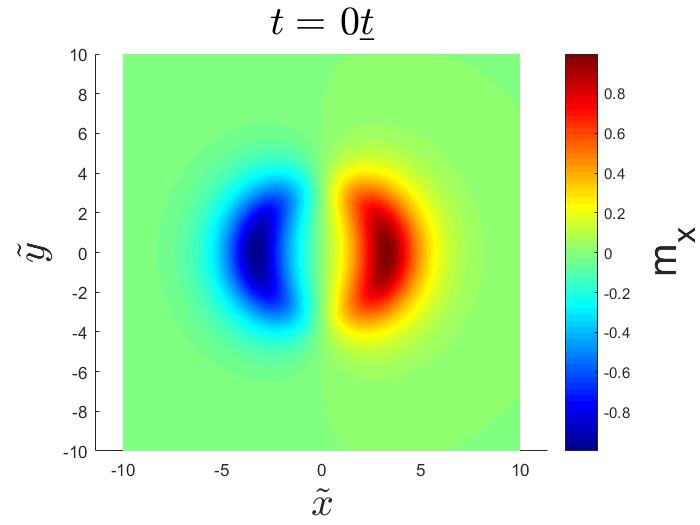
\includegraphics[width=\linewidth]{Figures/StaticSkyrmionMxT0.jpg}
  \caption{}
  \label{fig:StaticSkyrmionMxT0}
\end{subfigure}
\begin{subfigure}{.3\textwidth}
  \centering
  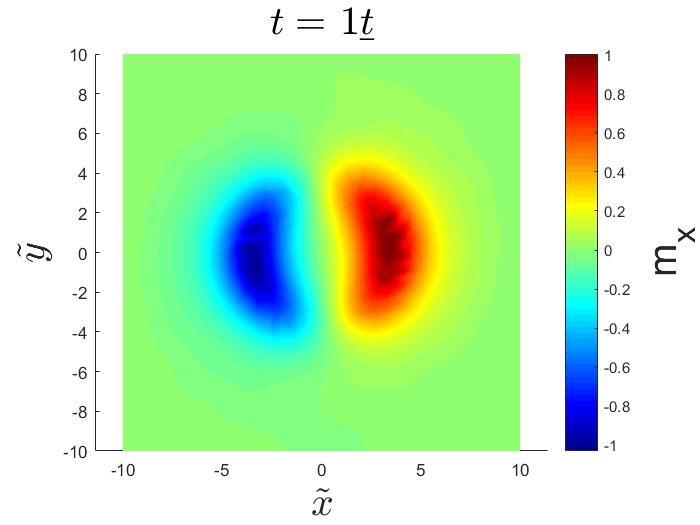
\includegraphics[width=\linewidth]{Figures/StaticSkyrmionMxT1.jpg}
  \caption{}
  \label{fig:StaticSkyrmionMxT1}
\end{subfigure}
\begin{subfigure}{.3\textwidth}
  \centering
  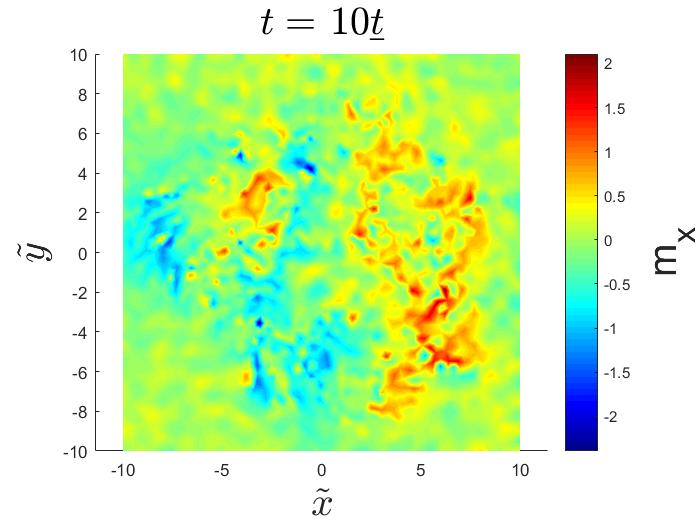
\includegraphics[width=\linewidth]{Figures/StaticSkyrmionMxT10.jpg}
  \caption{}
  \label{fig:StaticSkyrmionMxT10}
\end{subfigure}

\begin{subfigure}{.3\textwidth}
  \centering
  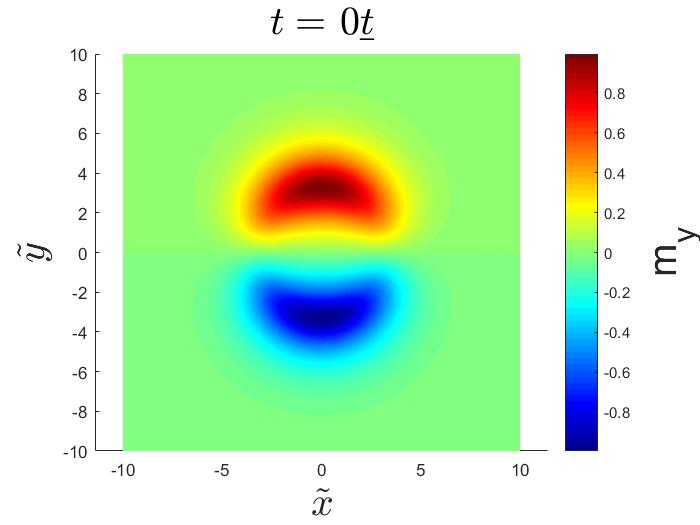
\includegraphics[width=\linewidth]{Figures/StaticSkyrmionMyT0.jpg}
  \caption{}
  \label{fig:StaticSkyrmionMyT0}
\end{subfigure}
\begin{subfigure}{.3\textwidth}
  \centering
  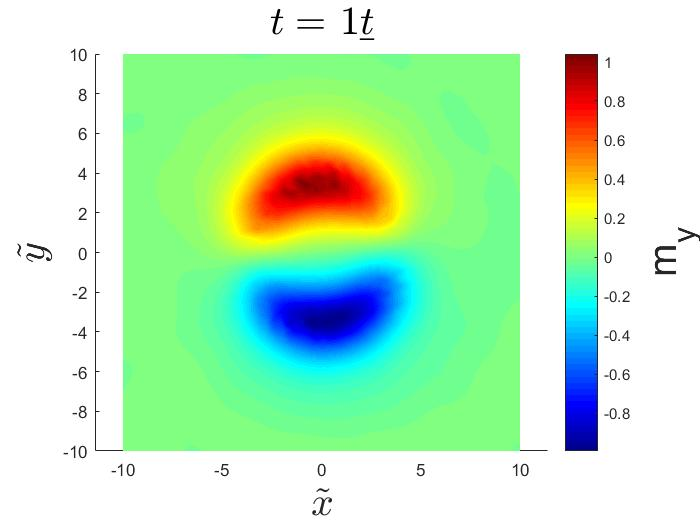
\includegraphics[width=\linewidth]{Figures/StaticSkyrmionMyT1.jpg}
  \caption{}
  \label{fig:StaticSkyrmionMyT1}
\end{subfigure}
\begin{subfigure}{.3\textwidth}
  \centering
  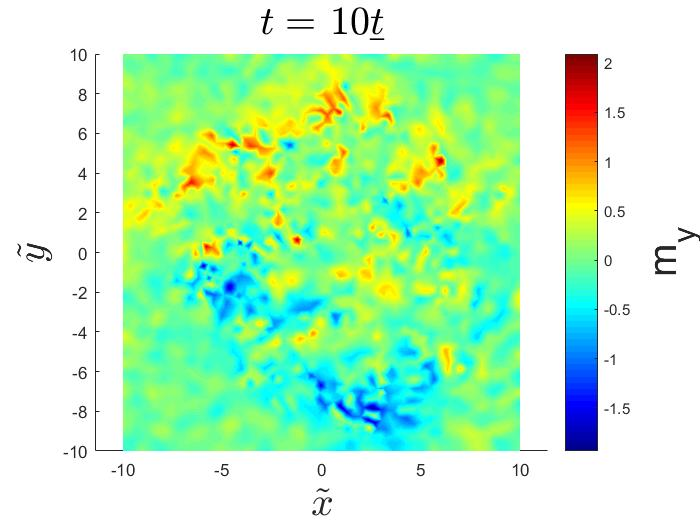
\includegraphics[width=\linewidth]{Figures/StaticSkyrmionMyT10.jpg}
  \caption{}
  \label{fig:StaticSkyrmionMyT10}
\end{subfigure}

\begin{subfigure}{.3\textwidth}
  \centering
  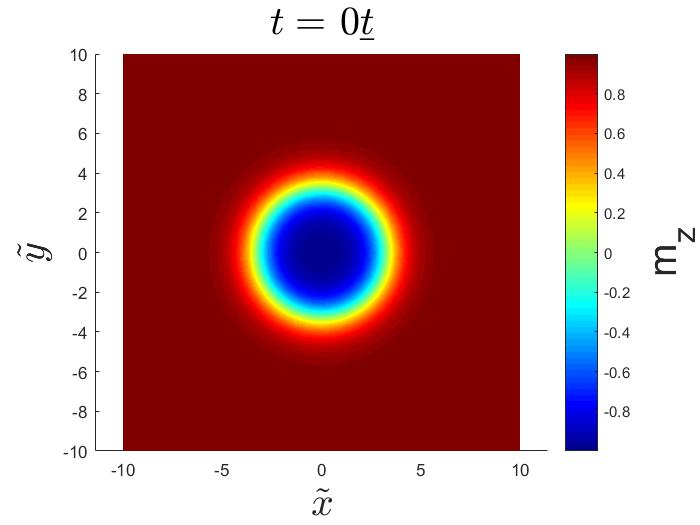
\includegraphics[width=\linewidth]{Figures/StaticSkyrmionMzT0.jpg}
  \caption{}
  \label{fig:StaticSkyrmionMzT0}
\end{subfigure}
\begin{subfigure}{.3\textwidth}
  \centering
  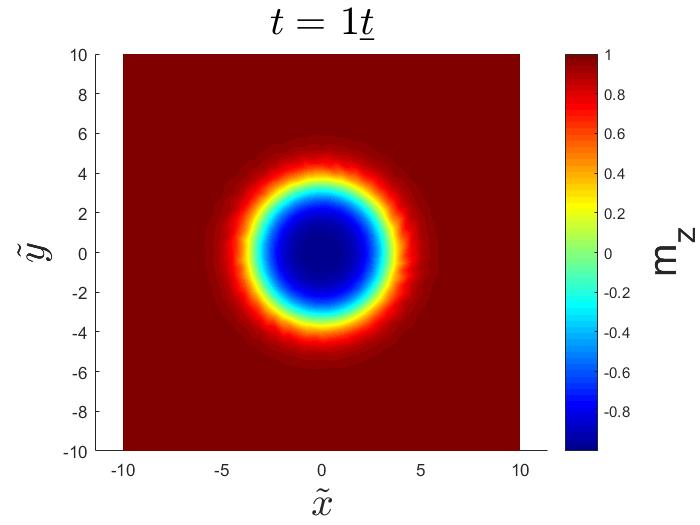
\includegraphics[width=\linewidth]{Figures/StaticSkyrmionMzT1.jpg}
  \caption{}
  \label{fig:StaticSkyrmionMzT1}
\end{subfigure}
\begin{subfigure}{.3\textwidth}
  \centering
  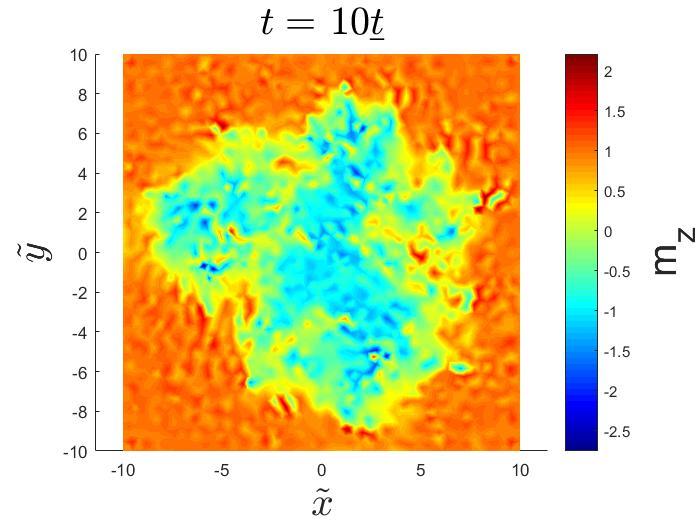
\includegraphics[width=\linewidth]{Figures/StaticSkyrmionMzT10.jpg}
  \caption{}
  \label{fig:StaticSkyrmionMzT10}
\end{subfigure}
\caption{Plots of the vector components $m_x$, $m_y$ and $m_z$ in the skyrmion plane for different times in the numerical simulation. The first row contains the data for $m_x$, the second for $m_y$ and the third for $m_z$. The first column shows the initial state, the second at a time $t=\underline{t}$ and the third at a time $t=10\underline{t}$.}
\label{fig:StaticSkyrmion}
\end{figure}
The results are shown in Figure \ref{fig:StaticSkyrmion}. At a time $t=\underline{t}$ there is not much change in the solution, but there is a slight counterclockwise rotation of the $m_x$ and $m_y$ values. After a time $t=10\underline{t}$, however, the solution has smeared out significantly from the initial state. More importantly, the values of the vector components exceed the allowed interval $\left[-1,1\right]$ by far, thereby breaking the normalization $m_x^2+m_y^2+m_z^2=1$ of the system. The LLG equation explicitly conserves the magnitude of the magnetization, so this is of particular interest when considering the stability of the code. Although we have three equations that we solve numerically, they are not independent of each other, as we can find the third vector component up to a sign once we have the solution of two. The numerical simulation does not seem to handle this well enough after a certain time, however. It is therefore a clear indication that the implemented solution method is not stable enough. There are several things that could cause this. If the boundary conditions are chosen incorrectly, this could affect the system. For this simulation Dirichlet boundary conditions corresponding to the numerical skyrmion solution at each point were chosen, and should therefore not affect the solution under the assumption that there is no dynamics. Another possible source of the instability is how the initial conditions are handled. The out of plane angle $\theta$ in the skyrmion profile has to be determined numerically from \eqref{eq:ODEtheta}. This is a differential equation with a singular point at $\tilde{r} = 0$, and we therefore settle by solving the equation down to a value close to zero. The solution of $\theta$ will also be needed arbitrarily close to zero, or at zero itself, when considering the entire skyrmion. A quick fix to this problem is shifting the $\tilde{r}$-values of the numerical solution of $\theta$ so that the $\theta$ values start at $\tilde{r}=0$ instead of $\tilde{r}=\epsilon$ (with $\epsilon$ here being set to $10^{-4}$). This is not a particularly good solution to the problem, as it introduces a small off-set to the solution of $\theta$ that will make the skyrmion profile not perfectly aligned with the effective field. However, as this off-set is so small, it is expected that any dynamics this will induce in the LLG equation will primarily go towards stabilizing the skyrmion to its proper stable form. What is more important about this fix is that it makes the function $\theta(\tilde{r})$ well defined at all points, so that $\mathbold{m} = \left(\sin\theta\cos\Phi,\sin\theta\sin\Phi,\cos\theta\right)$ is defined at all points in the skyrmion plane. To check if this fix is sufficient, we study the first and second derivatives of the magnetization, which appear in the effective field. The results are shown in Figure \ref{fig:SkyrmionDerivatives}.
\begin{figure}[h!]
\centering
\begin{subfigure}{.45\textwidth}
  \centering
  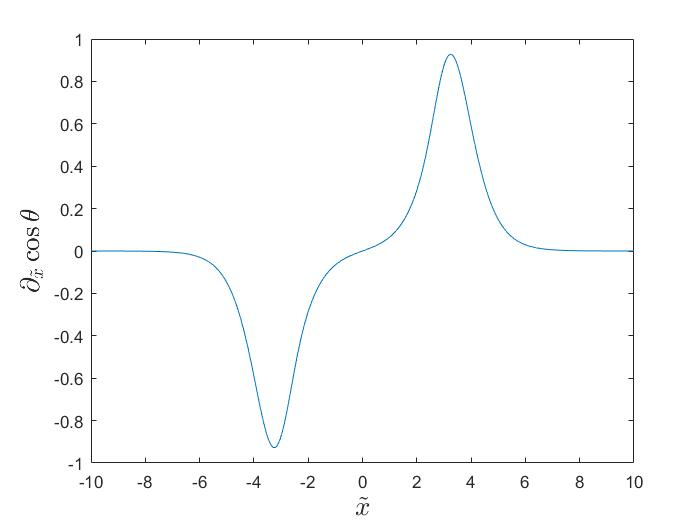
\includegraphics[width=\linewidth]{Figures/dCosTheta.jpg}
  \caption{}
\end{subfigure}
\begin{subfigure}{.45\textwidth}
  \centering
  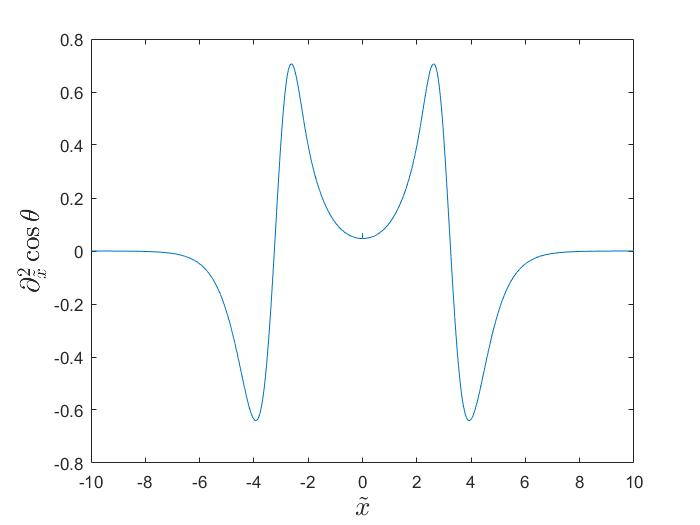
\includegraphics[width=\linewidth]{Figures/d2CosTheta.jpg}
  \caption{}
\end{subfigure}

\begin{subfigure}{.45\textwidth}
  \centering
  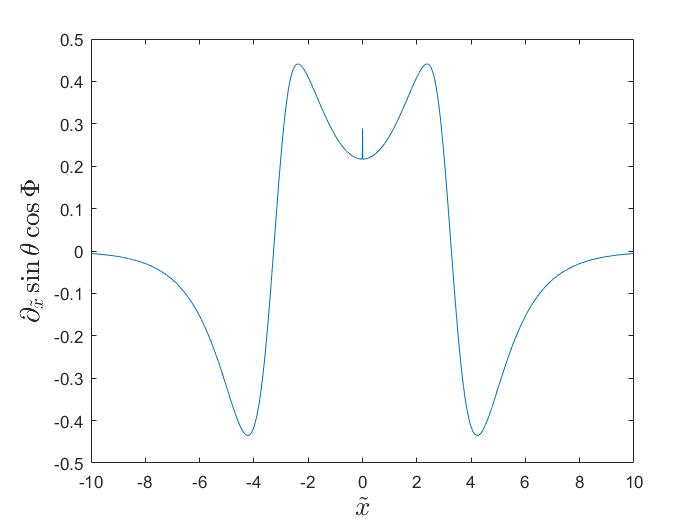
\includegraphics[width=\linewidth]{Figures/dSinThetaCosPhi.jpg}
  \caption{}
\end{subfigure}
\begin{subfigure}{.45\textwidth}
  \centering
  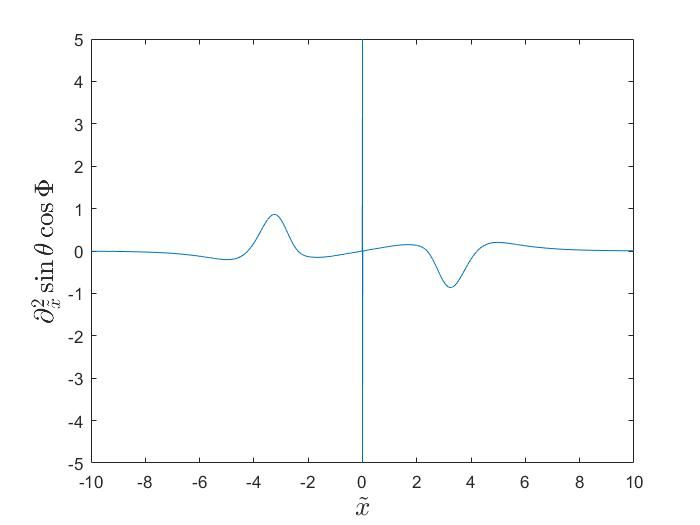
\includegraphics[width=\linewidth]{Figures/d2SinThetaCosPhi.jpg}
  \caption{}
\end{subfigure}
\caption{First and second derivatives of $m_x$ and $m_z$ in the $x$-direction. Every derivative has a discontinuity at $\tilde{x}=0$ except for the first derivative of $m_z$. The second derivative of $m_x$ has a singularity at $\tilde{x}=0$.}
\label{fig:SkyrmionDerivatives}
\end{figure}
As one can see, we still have an issue with discontinuities in the derivatives. For the $m_x = \sin\theta\cos\Phi$ case this could possibly stem from the $\cos\Phi$ factor, as $\Phi$ is not properly defined at $\tilde{r}=0$. As the first derivative of $m_x$ has a discontinuity while the first derivative of $m_z$ does not, and $m_z$ is independent of $\Phi$, it would back up this hypothesis. However, as $\sin\theta(\tilde{r}=0)=0$ a value for $\Phi$ at this point should not be necessary. But we also see that our fix of the $\theta$ solution cannot be without problems, as we also have a discontinuity in the second derivative of $m_z$, and this must stem from how we handle $\theta$. These discontinuities could therefore be an explanation for the instability in our numerical simulations. A last possible explanation for the instability is that while the LLG equation should conserve the magnitude of $\mathbold{m}$ by default due to the form of the equation, there is no explicit constriction in the solver that requires that $m_x^2+m_y^2+m_z^2=1$. As the numerical solutions are based on approximations, if there is a small perturbation that makes $m_x^2+m_y^2+m_z^2\neq1$ the solver will not necessarily attempt to adjust the magnitude of $\mathbold{m}$ back to unity, and this perturbation can then increase until the components of $\mathbold{m}$ reach unrealistic values. From this point on the results of the simulation are of absolutely no interest, as the input to the next time step is outright wrong.

\subsection{Spin-transfer torque driven dynamics}
In the previous subsection we saw that the numerical simulation proved to be unstable even in a case that should involve no dynamics. However, up to the time $t=\underline{t}$ it was more or less stable, with some deformations of the initial state that should not be present. Despite the fact that the results yielded by the simulations cannot be relied entirely upon, even up to this time, we will attempt to introduce some dynamical terms in the LLG equation and solve this to a time $t=\underline{t}$ and compare this with our analytical results. While the quantitative behavior may be too inaccurate for us to judge if the numerical results agree with our analytical ones, hopefully we can still see if the qualitative behavior is the same. 
\begin{figure}[h!]
\centering
\begin{subfigure}{.45\textwidth}
  \centering
  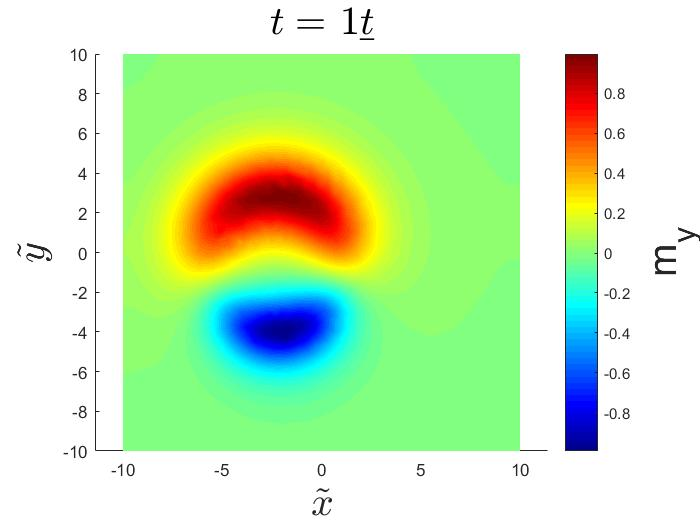
\includegraphics[width=\linewidth]{Figures/SkyrmionMySTTa1b3.jpg}
  \caption{}
\end{subfigure}
\begin{subfigure}{.45\textwidth}
  \centering
  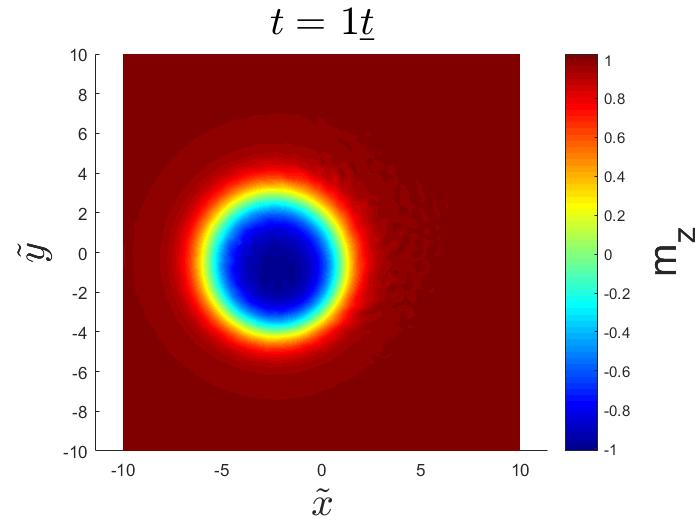
\includegraphics[width=\linewidth]{Figures/SkyrmionMzSTTa1b3.jpg}
  \caption{}
\end{subfigure}
\caption{Plots of $m_y$ and $m_z$ at a time $t=\underline{t}$ for a skyrmion driven by spin transfer torques. The skyrmion considered has $C=0.5551$ and the applied current gives a characteristic velocity $b_J\approx 178$ m/s ($b_J=1$ in dimensionless units). The values of the damping parameters were set to $\alpha=1.0$ and $\beta=3.0$. The geometric center of the skyrmion is found to be approximately $\left(-2.20, -0.85\right)$ from the plot of $m_z$.}
\label{fig:SkyrmionMotionSTTa1b3}
\end{figure}
The first test we do is on a skyrmion with $A=\SI{10}{pJ/m}$, $K=0.17$ MJ/m$^3$, $D=1.75$ mJ/m$^2$, $M_s=0.96$ MA/m. The characteristic velocity $b_J$ due to the spin transfer torque from the current is set to be unity in dimensionless units. Lastly we choose large damping parameter values ($\alpha=1.0$ and $\beta=3.0$) to make the impact of the different types of STT clear. The results are shown in Figure \ref{fig:SkyrmionMotionSTTa1b3}. While there is a clear deformation of the $m_y$ component, the $m_z$ component has more or less undergone a rigid motion, and all the magnetization components have reasonable values in the range $\left[-1,1\right]$. By looking closely at the plot of $m_z$ one can find that the location of the skyrmion core is approximately $\left(-2.20, -0.85\right)$. Using our analytical model in \eqref{eq:ElectricalSkyrmionVComponents} we would expect the core to be at $\left(-2.47, -0.88\right)$. The numerical result is then rather close to what we would expect from our analytical model. The discrepancy can perhaps be due to the deformation of the $m_y$ component, as our analytical model was made under the assumption of a rigid motion of the skyrmion. Whether the deformation is something that would actually occur in the physical case is not something we can say with accuracy, as we have already determined in the last subsection that the simulations give some deformations in cases where there should be none. In any case, the result we get agrees very well qualitatively with our analytical ones. We have a main velocity component along the direction of the conduction electrons, and also a component perpendicular to the current direction due to the skyrmion Hall effect as $\alpha\neq\beta$. When $\alpha=\beta$, however, we expect this perpendicular component from the skyrmion Hall effect to vanish. To check this we run a simulation with similar parameters as before, except now we set $\alpha=\beta=1$. The analytical model would now expect the skyrmion to have a velocity $\mathbold{v}=-b_J\mathbold{\hat{x}}$. The $m_z$ component resulting from this simulation is presented in Figure \ref{fig:SkyrmionMotionSTTa1b1}, and its center is at $\left(-1,0\right)$, in complete agreement with our analytical model. In addition, we do not have any deformations of significant magnitude in any of the magnetization components.
\begin{figure}[h!]
\centering
  \centering
  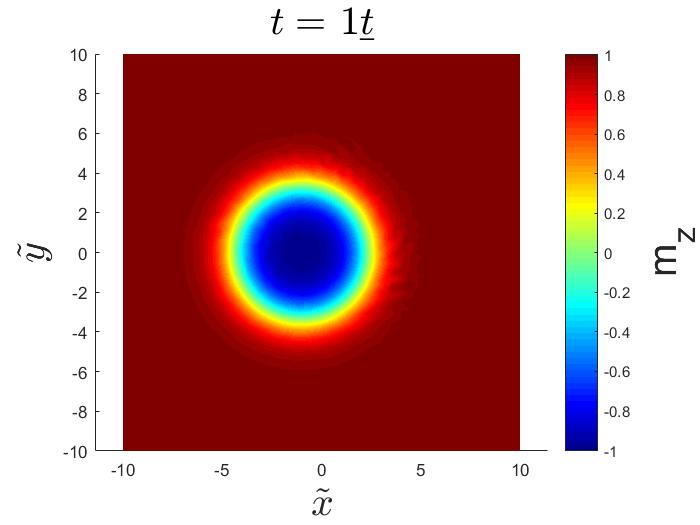
\includegraphics[width=.6\linewidth]{Figures/SkyrmionMzSTTa1b1.jpg}
\caption{Plot $m_z$ at a time $t=\underline{t}$ for a skyrmion driven by spin transfer torques. The skyrmion considered has $C=0.5551$ and the applied current gives a characteristic velocity $b_J\approx 178$ m/s ($b_J=1$ in dimensionless units). The values of the damping parameters were set to $\alpha=\beta=1.0$. The geometric center of the skyrmion is found to be $\left(-1, 0\right)$ from the plot of $m_z$.}
\label{fig:SkyrmionMotionSTTa1b1}
\end{figure}

\subsection{The effects of RSOC on the current driven dynamics}
We now move on to check the effects of RSOC on the dynamics of the skyrmion. It turns out that there is no time in the simulation that is large enough to see these effects that does not break the normalization of the magnetization to a significant degree. These values outside of the range $\left[-1,1\right]$ are local, however, so we still attempt an analysis. Before we start the analysis it should be noted that the results shown and discussed in this section should be taken with a grain of salt, as the code shows clear signs of instability. As this instability also appears at $t=\underline{t}$, and does not increase significantly at $t=2\underline{t}$, we run our simulation up to $t=2\underline{t}$ in this subsection. The dynamical effects of RSOC only appears when we have an applied current in the material. To see its effects it is therefore best to compare the current driven dynamics of a skyrmion in a material with and without RSOC. The strength of DMI is set to be the same in both systems, despite the fact that the presence of RSOC will influence this. For this simulation we use the data for the cobalt nanotracks in Table \ref{tab:PhysicalConstants}, and apply a current in the $x$-direction corresponding to $b_J = 1$ in its dimensionless value. We let the damping constants take on large values $\alpha=\beta=1$ for it to be easier to recognize the effects of RSOC, as it is expected that the RSOC correction is proportional to $\beta$. The simulation results are shown in Figure \ref{fig:SkyrmionRSOC}. The first thing we notice is that there is significant more deformation in the system with RSOC than the one without. This could again be due to the instability of the code, having RSOC present in the LLG equation makes the equations harder to solve. However, RSOC appears as fields in the LLG equation, and for large currents these fields can reach an order of magnitude comparable to the effective field. It is therefore not that unexpected that RSOC causes a deformation of the skyrmion, as the skyrmion magnetization profile is no longer perfectly aligned with the experienced magnetic field. The second thing one notices is that the location of the skyrmion core is not the same in the material with RSOC and the one without. The presence of RSOC shifts the core in the positive $x$- and $y$-direction. This is behavior that is similar to what is predicted by \eqref{eq:ElectricalSkyrmionVComponents} (remember that $R$ is negative for positive $\alpha_R$ and $b_J$). Analytically the core should be located at $\left(-1.17, 0.29\right)$ in the presence of RSOC, while numerically the core is approximately found to be located at $\left(-0.90, 0.35\right)$. The results are not that different, and can possibly be due to the deformation of the skyrmion or the instability of the code. What is most important to note is that the qualitative effects of RSOC on the current driven skyrmion dynamics agree rather well with one another.
\begin{figure}[h!]
\centering
\begin{subfigure}{.45\textwidth}
  \centering
  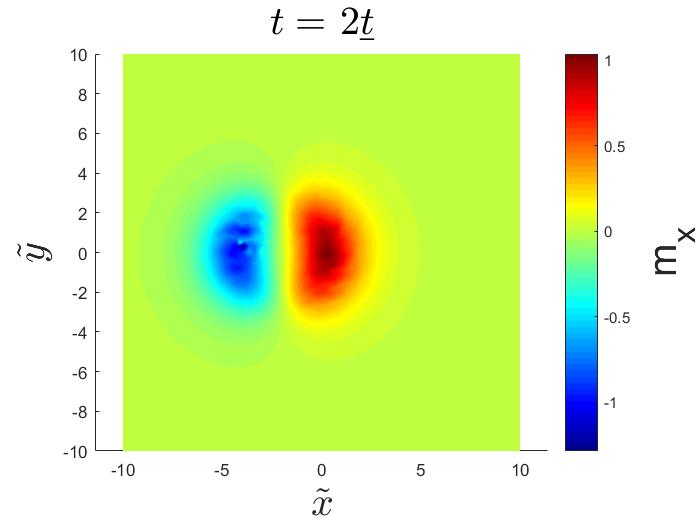
\includegraphics[width=\linewidth]{Figures/SkyrmionMxRSOCR0.jpg}
  \caption{}
\end{subfigure}
\begin{subfigure}{.45\textwidth}
  \centering
  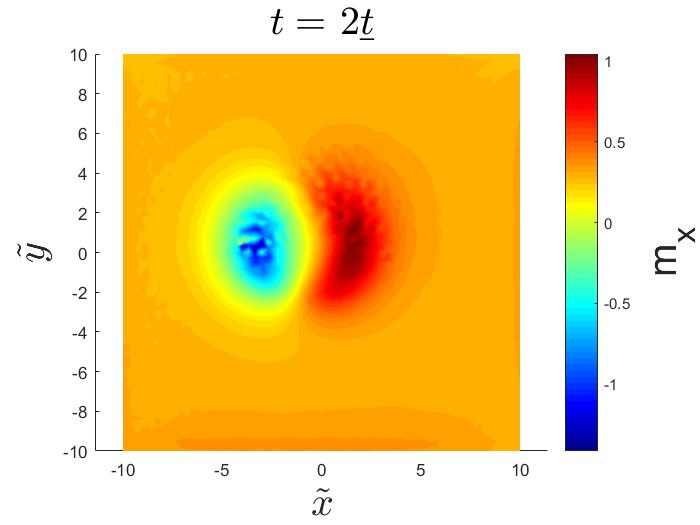
\includegraphics[width=\linewidth]{Figures/SkyrmionMxRSOC.jpg}
  \caption{}
\end{subfigure}

\begin{subfigure}{.45\textwidth}
  \centering
  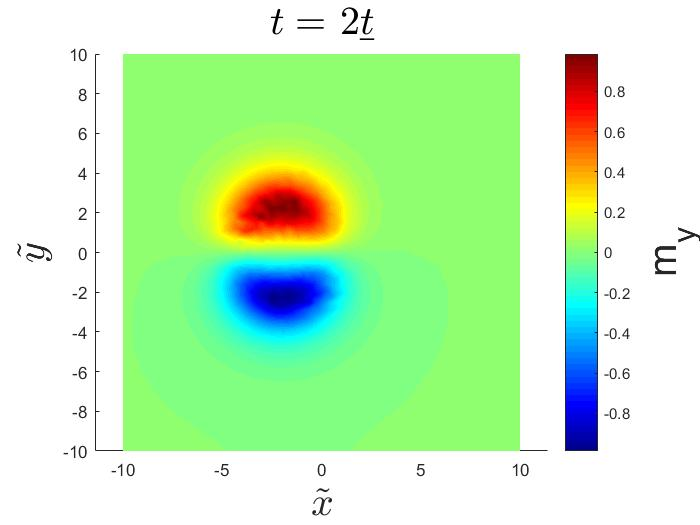
\includegraphics[width=\linewidth]{Figures/SkyrmionMyRSOCR0.jpg}
  \caption{}
\end{subfigure}
\begin{subfigure}{.45\textwidth}
  \centering
  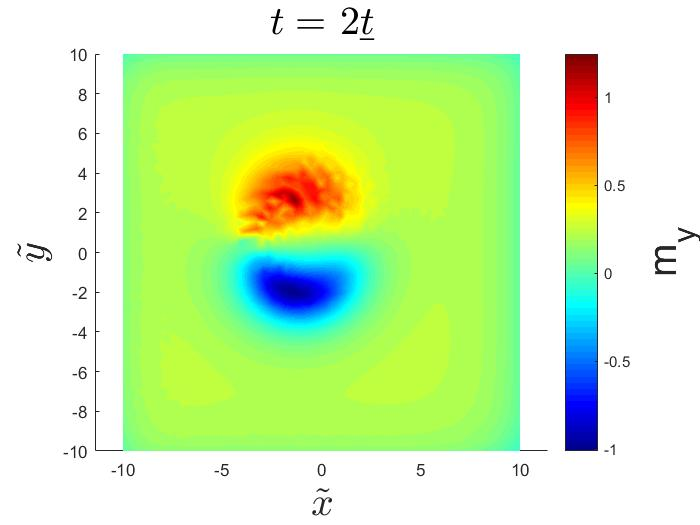
\includegraphics[width=\linewidth]{Figures/SkyrmionMyRSOC.jpg}
  \caption{}
\end{subfigure}

\begin{subfigure}{.45\textwidth}
  \centering
  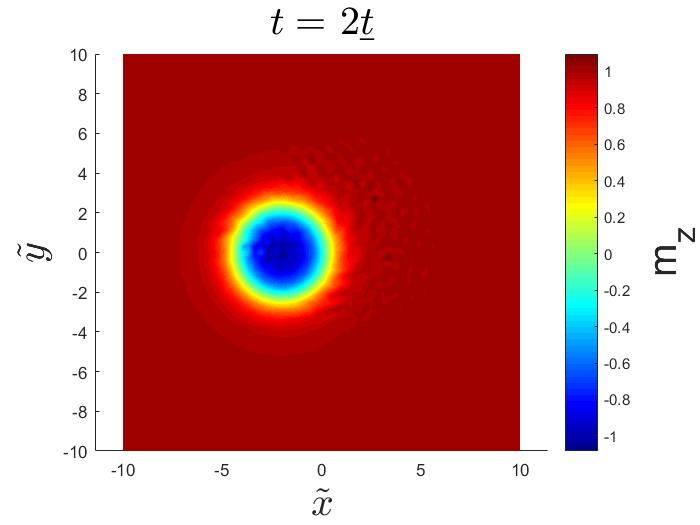
\includegraphics[width=\linewidth]{Figures/SkyrmionMzRSOCR0.jpg}
  \caption{}
\end{subfigure}
\begin{subfigure}{.45\textwidth}
  \centering
  \includegraphics[width=\linewidth]{Figures/SkyrmionMzRSOC.jpg}
  \caption{}
\end{subfigure}
\caption{$\alpha_R=5.1$ peV$\cdot$m, $b_J=1$, $C=0.75$, $\alpha=\beta=1$. The skyrmion core is located at $\left(-2,0\right)$ without RSOC, and at approximately $\left(-0.90,0.35\right)$ with RSOC. }
\label{fig:SkyrmionRSOC}
\end{figure}

\subsection{Electric field driven dynamics}
The last effect to check numerically is then the dynamics induced by an inhomogeneous electric field applied perpendicular to the skyrmion plane. The problem with simulating these effects is that for reasonably scaled electric field gradients, such that the overall change in the free energy in the vicinity of the skyrmion is rather small, the time scale needed to see the effects is quite large compared to $\underline{t}$. At these time scales we have seen that the simulations become unstable, and this instability renders any output we may get useless. To get a motion of the skyrmion that we can see at a time scale $\underline{t}$ we can, however, use a very steep electric field gradient. The ones used in these simulations were set so that $\eta E_{x/y}\underline{r} = 0.2 K$. This method is not entirely unproblematic either, not even considering that this is a much stronger modification of the anisotropic energy than we can accomplish with an electric field. With a gradient this steep there is a considerable change in the free energy. If we consider the example with $\eta E_{x}\underline{r} = 0.2 K$ the total anisotropic energy at $\tilde{x}=-5$ is zero, while at $\tilde{x}=5$ is twice that of the original anisotropic energy without an applied electric field. This should cause noticeable deformations in the skyrmion, as the change in the effective field becomes so great that the magnetization of the skyrmion is not even close to being the stable solution. For small time scales these deformations will hopefully not be that dominant, however. There are two effects we would like to check for the electric field driven motion of the skyrmion; in the undamped limit the skyrmion should move perpendicular to the electric field gradient, while in the presence of damping there should also be a velocity component in the opposite direction of the gradient. We therefore run simulations for two different values of $\alpha$ for each gradient direction. We choose a value $\alpha=0.01$ that should show primarily the motion in the undamped case, and a value $\alpha=0.7$ to introduce the velocity component due to damping. The value of $\alpha=0.7$ is chosen to get the maximum velocity component in the opposite direction of the field gradient. This happens when $\alpha_C=1$, which would correspond to $\alpha=0.7$ for a skyrmion with $C=0.75$, as we get when using the values for the cobalt nanotracks in Table \ref{tab:PhysicalConstants}. The simulation results for the $m_z$ component at a time $t=2\underline{t}$ are shown in Figure \ref{fig:SkyrmionEField}. As we can see there is some deformation of the skyrmion, primarily an elongation along the axis where we apply an electric field gradient. If one studies the plots closer, one can also see that the position of the core has moved slightly, although this is hard to see directly from the plots as presented here.

We will now compare the analytical and numerical core positions using \eqref{eq:ElectricalSkyrmionVComponents} and Figure \ref{fig:SkyrmionEField}. The analytical core locations are given by $\left(-0.01, -0.86\right)$ and $\left(-0.43, -0.43\right)$ for a gradient in the $x$-direction and a damping parameter $\alpha=0.01$ and $\alpha=0.7$ respectively. For a gradient in the $y$-direction the locations are $\left(0.86,-0.01\right)$ and $\left(0.43, -0.43\right)$ for $\alpha=0.01$ and $\alpha=0.7$ respectively. The analytical results are in good agreement with the velocity component perpendicular to the gradient found numerically, but there is some discrepancy in the velocity component in the opposite direction of the gradient that is proportional to $\alpha$. Qualitatively the damped velocity component behaves correctly, but quantitatively it is a bit off comparing to the perpendicular velocity component. This could possibly stem from the elongation of the skyrmion along the gradient axis, as the core is chosen to be where the $m_z$ component is minimal, but this is no longer the geometric center of the skyrmion. 
\begin{figure}[h!]
\centering
\begin{subfigure}{.45\textwidth}
  \centering
  \includegraphics[width=\linewidth]{Figures/SkyrmionExA001.jpg}
  \caption{}
\end{subfigure}
\begin{subfigure}{.45\textwidth}
  \centering
  \includegraphics[width=\linewidth]{Figures/SkyrmionExA07.jpg}
  \caption{}
\end{subfigure}

\begin{subfigure}{.45\textwidth}
  \centering
  \includegraphics[width=\linewidth]{Figures/SkyrmionEyA001.jpg}
  \caption{}
\end{subfigure}
\begin{subfigure}{.45\textwidth}
  \centering
  \includegraphics[width=\linewidth]{Figures/SkyrmionEyA07.jpg}
  \caption{}
\end{subfigure}
\caption{The $m_z$ component of a skyrmion with $C=0.75$ at a time $t=2\underline{t}$ after applying an electric field gradient to the system at $t=0$. In \textbf{(a)} and \textbf{(b)} we have applied a gradient $E_x$ in the $x$-direction, while in \textbf{(c)} and \textbf{(d)} we have applied a gradient $E_y$ in the $y$-direction. The electric field is given by $E = (E_x x+E_yy)\mathbold{\hat{z}}$, and the field strength is given by $\eta E_{x/y}\underline{r} = 0.2 K$, where we have used the materialistic properties of cobalt nanotracks. In \textbf{(a)} and \textbf{(c)} the damping parameter is $\alpha = 0.01$, while in \textbf{(b)} and \textbf{(d)} it is $\alpha=0.7$. The core locations are found to be approximately \textbf{(a)} $\left(0,-0.75 \right)$, \textbf{(b)} $\left(-0.2,-0.4 \right)$, \textbf{(c)} $\left(0.75,0 \right)$, \textbf{(d)} $\left(0.4,-0.2 \right)$.}
\label{fig:SkyrmionEField}
\end{figure}

As a final comment on the electric field control of the skyrmion motion we would like to discuss what is a realistic size of the electric field gradient, and how this may be utilized in skyrmion motion. By rewriting \eqref{eq:ElectricalSkyrmionVComponents}, we can express the electric field gradients as
\begin{subequations}
\begin{align}
    E_x &= -\frac{1}{C_E}\left[\left(\beta_C+R\right)b_J + \alpha_C\dot{x}_0+\dot{y}_0\right], \\
    E_y &= \frac{1}{C_E}\left[b_J+\dot{x}_0-\alpha_C\dot{y}_0\right].
\end{align}
\end{subequations}
One use of the electric field control of the skyrmion motion is to cancel out the perpendicular velocity component when the skyrmion is dynamically driven by a spin-polarized current. We can then estimate the size of the gradient necessary to accomplish this based on the expression above. For simplicity we assume a case with $\alpha=0$, so that the $\dot{y}_0$ component can be cancelled out by an electric field gradient in the $x$-direction alone. The value of $\beta$ needs to be nonzero for us to have a nonzero $\dot{y}_0$ to cancel out. In this example we let $\beta=0.01$ for reference, and we note that the field gradient scales linearly with $\beta$. The magnitude of the electric field gradient in the $x$-direction necessary to make $\dot{y}_0$ vanish then becomes
\begin{align}
    \eta E_x\underline{r} = -\frac{2\mu_0M_s\underline{r}}{\gamma' I_3}\left(\beta_C+R\right)b_J.
\end{align}
For a current density $j_e = 10^{10}$ A/m$^2$ the size of $b_J$ is approximately $\SI{1}{m/s}$. In the cobalt nanotrack case, we would then require an electric field gradient of the magnitude $\eta E_x\underline{r}/K = -2.8\cdot10^{-6}$ to cancel out the perpendicular velocity component, while for the Ir|Co|Pt multilayer system we would require $\eta E_x\underline{r}/K = -1.2\cdot10^{-5}$. This is a much more feasible field gradient than the one used in the numerics to illustrate the dynamics (which was $\eta E_x\underline{r}/K = 0.2$), as it does not require a very considerable change in the perpendicular magnetic anisotropy. In addition, as the free energy is slowly varying in the vicinity of the skyrmion, it is unlikely to cause any deformations of significance. 

\chapter{Spin torque oscillators}
\section{Giant magnetoresistance}
An important effect that is fundamental for the spin torque oscillators is the giant magnetoresistance (GMR) effect. This effect was discovered by Albert Fert \cite{Fert1988} and Peter Gr\"{u}nberg \cite{Grunberg1989} in 1988, for which they won the Nobel prize in 2007. They discovered that when an electrical current passed through a layered magnetic system with different magnetic orientations, the resistance changed considerably depending on whether the magnetic layers were parallel or anti-parallel, as illustrated in Figure \ref{fig:GMR}. The reason for this difference in resistance is that electrons with magnetic moments aligned with the local magnetization are scattered far less than electrons that have a component in their magnetic moments that is perpendicular to the local magnetization \cite{Chappert2007}. This can be argued through the fact that in the ferromagnetic coupling between the itinerant and local electrons, the electrons that are not aligned with the local magnetization have a higher exchange energy than electrons that are aligned. They then have to pass through a higher energy barrier than the aligned electrons, and the current of those electrons will therefore have a higher resistance.
\begin{figure}[h!]
\centering
  \begin{subfigure}[b]{.58\textwidth}
  \includegraphics[width=\linewidth]{Figures/GMR_AP.pdf}
  \caption{}
  \label{fig:GMR_AP}
\end{subfigure}
\begin{subfigure}[b]{.6\textwidth}
  \includegraphics[width=\linewidth]{Figures/GMR_P.pdf}
  \caption{}
  \label{fig:GMR_P}
\end{subfigure}
\caption{The resistance of a current passing through a multilayered magnetic system depends on the magnetic moment of the electron (proportional to their spin) and the alignment of the magnetic layers. Here we consider an anti-parallel configuration in \textbf{(a)} and a parallel configuration in \textbf{(b)} separated by a non-magnetic material. In \textbf{(a)} the resistance is high because of the anti-parallel configuration of the magnetic layers the current has to pass through. In \textbf{(b)} the resistance of the electrons with a magnetic moment parallel to the magnetic layers is lower than the electrons with an anti-parallel magnetic moment.}
\label{fig:GMR}
\end{figure}

GMR has most noticeably been utilized in nonvolatile memory technologies such as magnetoresistive random-access memory (MRAM) \cite{Akerman2005} and racetrack memories \cite{Parkin2008}. The GMR is pivotal in spin torque oscillators, as the resistance is a function of the angle between two magnetizations. If we were able to make these magnetizations oscillate, such that the angle between them varies in time, the oscillation in the resistance due to GMR will cause an oscillation in the current. We would then have an oscillator that converts the direct current applied to the system into an alternating current. This type of system that utilizes the precession of magnetic moments to generate an oscillating current is known as a spin torque oscillator (STO).

\section{Spin torque oscillators under influence of spin--orbit coupling}
The spin torque oscillators that we will consider in this thesis primarily consist of a fixed polarizing magnetic layer, and two free magnetic layers that interact with each other through the RKKY interaction. We will study the effects the Rashba spin--orbit coupling may have in two different geometries, a bulk geometry and a thin film geometry, as illustrated in Figure \ref{fig:Geometries}. Whether the system is in an oscillating state depends on the system parameters, such as the strength of the magnetic anisotropy (which we assume to be uniaxial), the current density inducing spin-transfer torques, and the strength of the RKKY interaction between the free magnetic layers. Spin torque oscillators have been found to occur in both ferromagnetic \cite{Zhou2013} and antiferromagnetic \cite{Klein2012} coupling between the free magnetic layers. By varying some of these parameters we can study when the system is in an STO phase, or when a collinear state where the free magnetic layers are aligned or anti-aligned with the easy axis of the material is stable. This would result in a phase diagram that would give information regarding what state we will find the system in for a given set of parameters. The goal of this chapter is to study the effects of Rashba spin--orbit coupling on the STO phase in this phase diagram, and the effects it has on the oscillation frequency of the current going out of the system. 
\begin{figure}[h!]
\centering
%\begin{center}
\begin{subfigure}{.6\textwidth}
  \begin{tikzpicture}
\node[above right] (img) at (0,0) {\includegraphics[width=1\textwidth]{Figures/STO_Bulkv2}};
\node at (10pt,70pt) {\Large{$z$}};
\node at (32pt,47pt) {\Large{$y$}};
\node at (42pt,8pt) {\Large{$x$}};
\node at (115pt,40pt) {\Large{F$_0$}};
\node at (192pt,40pt) {\Large{F$_1$}};
\node at (215pt,40pt) {\Large{F$_2$}};
\node at (70pt,110pt) {\textcolor{blue}{\Large{$\mathbold{j}_x$}}};
\node at (255pt,130pt) {\textcolor{blue}{\Large{$\mathbold{j}_y$}}};
\end{tikzpicture}
\caption{}
\label{fig:BulkGeometry} 
\end{subfigure}

\begin{subfigure}{.6\textwidth}
  \begin{tikzpicture}
\node[above right] (img) at (0,0) {\includegraphics[width=1\textwidth]{Figures/STO_Filmv2}};
\node at (8pt,50pt) {\Large{$z$}};
\node at (28pt,32pt) {\Large{$y$}};
\node at (37pt,-2pt) {\Large{$x$}};
\node at (90pt,25pt) {\Large{F$_0$}};
\node at (177pt,25pt) {\Large{F$_1$}};
\node at (212pt,25pt) {\Large{F$_2$}};
\node at (160pt,54pt) {\textcolor{blue}{\large{$\mathbold{j}_x$}}};
\end{tikzpicture}
\caption{}
\label{fig:FGeometry} 
\end{subfigure}
%\end{center}
\caption{Illustrations of \textbf{(a)} the bulk geometry and \textbf{(b)} the thin film geometry. In geometries a fixed magnetic layer F$_0$ is separated from two free magnetic layers F$_1$ and F$_2$ by a non-magnetic metallic material shown here in blue. A material illustrated in black, which is neighboring to F$_1$ and F$_2$ in \textbf{(a)} and the top film in \textbf{(b)}, is present to get a strong Rashba spin--orbit coupling at the interface of the free ferromagnetic layers. In \textbf{(b)} the bottom film is a material that will cause little to no RSOC at the interface to the ferromagnetic materials. To induce dynamics a current is applied in the $x$-direction which causes $\mathbold{m}_1$ and $\mathbold{m}_2$ to experience spin-transfer torques. In \textbf{(a)} a current is also applied in the $y$-direction to create significant RSOC effects on $\mathbold{m}_1$ and $\mathbold{m}_2$ due to the symmetry breaking in the $x$-direction. In the film geometry this is caused by the current in the $x$-direction as the symmetry breaking is in the $z$-direction. The free magnetic layers also interact through the RKKY interaction, while the distance to the fixed magnetic layer is chosen such that an RKKY interaction with this layer can be neglected. In \textbf{(a)} the material has an easy axis in the $z$-direction, while in \textbf{(b)} the material has an easy axis in the $y$-direction.}
\label{fig:Geometries}
\end{figure}

The model that we will use to analyze this system is a variation of the Landau--Lifshitz--Gilbert--Slonczewski (LLGS) equation that includes the Rashba field derived by Kim et al. \cite{Kim2012}. The LLGS equation is an expansion of the LLG equation \eqref{eq:LLG} that includes spin-transfer torques on uniform magnetic moments. Usually the non-adiabatic spin-transfer torque is rather small compared to the adiabatic spin-transfer torque, to an order of magnitude on the size of the Gilbert damping $\alpha$ (which is typically $~10^{-2}$ for the systems we will consider). This torque still has a significant contribution to the dynamics of the magnetization even at this order of magnitude, as we have previously seen in the skyrmion dynamics. In metallic multilayers such as N/F/N/F/N (N being a non-magnetic metal, and F being a ferromagnetic metal), however, the non-adiabatic STT is even smaller than usual due to symmetry considerations. The lowest contribution to the non-adiabatic STT in such a system becomes quadratic in the applied voltage bias $V$ that generates the current responsible for STT. Since the voltage bias necessary to generate large current densities for systems at this scale is quite small, a torque that is proportional to $V^2$ can be neglected. This symmetry consideration is discussed in more detail by Ralph and Stiles \cite{Ralph2008}. We are then content by only including the adiabatic spin-transfer torque in our model, and the LLGS equation that we consider then becomes
\begin{align}
    \label{eq:LLGS}
    \partial_t \mathbold{m}_i = -\gamma \mathbold{m}_i\times\left(\mathbold{H}^{\text{eff}}_i+\mathbold{H}^{\text{R}}_i - \beta\mathbold{m}_i\times\mathbold{H}^{\text{R}}_i\right) + \alpha\mathbold{m}_i \times\partial_t\mathbold{m}_i + \mathbold{T}^{\text{STT}}_i,
\end{align}
with $\mathbold{m}_i$ being the magnetization in F$_i$. We remember that the Rashba field is given by
\begin{align}
    \mathbold{H}^{\text{R}}_i = \frac{1}{1+\beta^2}\frac{\alpha_{\text{R}}m_e P(i) j}{e M_s \hbar \mu_0} \mathbold{\hat{n}}\times\mathbold{\hat{j}}.
\end{align}
The polarization $P(i)$ is the polarization of the current responsible for the spin--orbit coupling at the interface between F$_i$ and the material that induces a strong RSOC at the interface. Note that the non-adiabatic contribution of the Rashba field proportional to $\beta$ is still included, as the same symmetry argument that allowed us to neglect the non-adiabatic STT is not applicable to this torque. The adiabatic STT acting on $\mathbold{m}_1$ and $\mathbold{m}_2$ are given by
\begin{subequations}
\begin{align}
    \mathbold{T}^{\text{STT}}_1 &= -\frac{\gamma \hbar j_x}{2 e M_s \mu_0 d} \mathbold{m}_1\times\left( P_0\mathbold{m}_0 - P_1 \mathbold{m}_2\right) \times \mathbold{m}_1, \\
    \mathbold{T}^{\text{STT}}_2 &= -\frac{\gamma \hbar j_x}{2 e M_s \mu_0 d} P_1 \mathbold{m}_2\times \mathbold{m}_1 \times \mathbold{m}_2,
\end{align}
\end{subequations}
following the derivation in Section \ref{sec:AdSTT}. Here $P_i$ is the polarization of the current after having passed through F$_i$. The effective field $\mathbold{H}^{\text{eff}}_i$ in the free magnetic layer F$_i$ is given by the field resulting from magnetic anisotropy and the RKKY interaction, which becomes
\begin{align}
    \mathbold{H}^{\text{eff}}_i = \frac{2K}{\mu_0 M_s}\left( \mathbold{m}_i \cdot \mathbold{\hat{n}}_k\right)\mathbold{\hat{n}}_k + \frac{J_{\text{RKKY}}}{\mu_0 M_s d} \mathbold{m}_{\bar{i}}.
\end{align}
Here $\mathbold{\hat{n}}_k$ is a unit vector along the easy axis, $d$ is the thickness of the free magnetic layers F$_1$ and F$_2$ (which are assumed to have an equal thickness), and $\bar{i}$ indicates the index of the free magnetic layer that is not $i$ ($\bar{i} = 3 - i$). To study the different stable phases of this system, which we assume to be collinear states along $\mathbold{\hat{n}}_k$, we follow the derivation by Zhou et al. \cite{Zhou2013}. We first make the ansatz that we have a small perturbation $\mathbold{u}_i$ from a collinear state, so that $\mathbold{m}_i \approx \lambda_i\mathbold{\hat{n}}_k + \mathbold{u}_i$, where $\lambda_i = \pm 1$. The possible collinear states in question are $\downarrow\downarrow, \downarrow\uparrow, \uparrow\downarrow, \uparrow\uparrow$, with the arrows indicating the direction of $\mathbold{m}_1$ and $\mathbold{m}_2$ respectively, and $\uparrow$ being the unit vector $\mathbold{\hat{n}}_k$ along the easy axis. To decide whether the collinear state is stable, we must study the time evolution of the perturbation $\mathbold{u}_i$. This is done by performing a Fourier transform of the LLGS equation using our ansatz of $\mathbold{m}_i$, which is shown in Appendix \ref{app:FourierLLGS}. The end result can be written compactly as
\begin{align}
    \label{eq:EigenvalueEqn}
    \left(\hat{A}\omega + \hat{V}\right)
    \begin{pmatrix}
     \tilde{\mathbold{u}}_1 \\
     \tilde{\mathbold{u}}_2
    \end{pmatrix}
    = 0.
\end{align}
The matrices for the different geometries are given by
\begin{subequations}
\begin{align}
    \hat{A}_{\text{bulk}} &=
    \begin{pmatrix}
     1-i\alpha\lambda_1 & 0 \\
     0 & 1-i\alpha\lambda_2
    \end{pmatrix}, \label{eq:Abulk}\\
    \hat{A}_{\text{film}} &=
    \begin{pmatrix}
     1+i\alpha\lambda_1 & 0 \\
     0 & 1+i\alpha\lambda_2
    \end{pmatrix}, \label{eq:Afilm}\\
    \nonumber\hat{V}_{\text{bulk}} &=
    \omega_0\begin{pmatrix}
     \lambda_1 & 0 \\
     0 & \lambda_2
    \end{pmatrix}
    + \omega_J \begin{pmatrix}
     \lambda_2 & -\lambda_1 \\
     -\lambda_2 & \lambda_1
    \end{pmatrix}
    + i\omega_j^{(x)}\left[P_0
    \begin{pmatrix}
     -\lambda_1 & 0 \\
     0 & 0
    \end{pmatrix}
    + P_1
    \begin{pmatrix}
     \lambda_1\lambda_2 & -1 \\
     1 & -\lambda_1\lambda_2
    \end{pmatrix}\right] \\
    &\hspace{4.5mm} \frac{\omega_R^{(y)}}{1+\beta^2}\left[
    \begin{pmatrix}
     P_1^{(y)} & 0 \\
     0 & P_2^{(y)}
    \end{pmatrix}
    - i \beta
    \begin{pmatrix}
     P_1^{(y)}\lambda_1 & 0 \\
     0 & P_2^{(y)}\lambda_2
    \end{pmatrix}\right], \label{eq:Vbulk}\\
    \nonumber\hat{V}_{\text{film}} &=
    -\omega_0\begin{pmatrix}
     \lambda_1 & 0 \\
     0 & \lambda_2
    \end{pmatrix}
    - \omega_J \begin{pmatrix}
     \lambda_2 & -\lambda_1 \\
     -\lambda_2 & \lambda_1
    \end{pmatrix}
    + i\omega_j^{(x)}\left[P_0
    \begin{pmatrix}
     -\lambda_1 & 0 \\
     0 & 0
    \end{pmatrix}
    + P_1
    \begin{pmatrix}
     \lambda_1\lambda_2 & -1 \\
     1 & -\lambda_1\lambda_2
    \end{pmatrix}\right] \\
    &\hspace{4.5mm} -\frac{\omega_R^{(x)}}{1+\beta^2}\left[
    \begin{pmatrix}
     P_0 & 0 \\
     0 & P_1
    \end{pmatrix}
    + i \beta
    \begin{pmatrix}
     P_0\lambda_1 & 0 \\
     0 & P_1\lambda_2
    \end{pmatrix}\right]. \label{eq:Vfilm}
\end{align}
\end{subequations}
Here we have defined the frequencies $\omega_0 = 2\gamma K/\mu_0M_s$, $\omega_J = \gamma J_{\text{RKKY}}/\mu_0 M_s d$, $\omega_j^{(x)} = \gamma \hbar j_x/2\mu_0M_sd$ and $\omega_R^{(x/y)} = \gamma \alpha_R m_e j_{x/y}/\hbar\mu_0 e M_s$. $\tilde{\mathbold{u}}_1$ and $\tilde{\mathbold{u}}_2$ are the Fourier transforms of $\mathbold{u}_1$ and $\mathbold{u}_2$, which is defined as $\mathbold{u}_i(t) = \int \tilde{\mathbold{u}}_i(\omega) \exp\left(-i\omega t\right) \d \omega/{2\pi}$. From this definition we can see that the perturbation is stable when the imaginary part of $\omega$ is less than zero, but when the imaginary part of $\omega$ is greater than zero the perturbation is exponentially increasing. To determine the sign of the imaginary component of $\omega$ we use \eqref{eq:EigenvalueEqn}. By rearranging the terms and multiplying with the inverse of $\hat{A}$, we see that $\omega$ is restricted to be one of the two possible eigenvalues of the $2\times2$ matrix $\hat{W} = -\hat{A}^{-1}\hat{V}$. The collinear state $\mathbold{m}_1=\lambda_1\mathbold{\hat{n}}_k$, $\mathbold{m}_2=\lambda_2\mathbold{\hat{n}}_k$ is then stable if both of the eigenvalues of $\hat{W}$ have negative imaginary components. This is of course dependent on the system parameters. We can then use this matrix to find the phase diagrams for when the collinear states are stable or not. There will be a region where none of the collinear states are stable for some choice of parameters, and it is in this region that an STO phase will have to be localized. However, a lack of a stable collinear state does not indicate that we have an STO phase. Our analytical model can only describe if a perturbation from a collinear state will increase or relax back to its original state, and if the perturbation is increasing it is not able to say whether the perturbation at some point becomes a self-sustained precession in the magnetization. 

Something else that we need to consider is what defines an STO phase. The goal of the spin torque oscillator is to transform the applied direct current into an alternating current, utilizing the giant magnetoresistance effect. The resistance of our multilayer system is dependent on the respective alignment of the magnetic layers, so when we excite oscillations in the magnetizations we get an oscillating resistance of the system. The resistance is approximated by
\begin{align}
    R(t) = R_0 + \Delta R_1\mathbold{m}_0\cdot\mathbold{m}_1 + \Delta R_2\mathbold{m}_1\cdot\mathbold{m}_2.
\end{align}
To have a spin torque oscillator we must therefore require oscillations in at least $\mathbold{m}_0\cdot\mathbold{m}_1$ or $\mathbold{m}_1\cdot\mathbold{m}_2$. Oscillations in $\mathbold{m}_1$ in the form of a precession around the axis of $\mathbold{m}_0$ will therefore not cause any change in the resistance of the system, and such oscillations are hence not considered as an STO phase. We will therefore later establish numerically based on the time evolution of $\mathbold{m}_1$ and $\mathbold{m}_2$ when we have an STO phase in our system.

Before moving on to numerics, we want to see if it is possible to find an analogy for the new terms in the LLGS equation that the Rashba field introduces. We see that the matrix proportional to $\omega_R$ in \eqref{eq:Vbulk} and \eqref{eq:Vfilm} is very similar to the $\hat{A}$ matrix in \eqref{eq:Abulk} and \eqref{eq:Afilm} in the case when $P_0=P_1$ and $P_1^{(y)}=P_2^{(y)}$. If we consider this case, we can incorporate the effects of RSOC into \eqref{eq:EigenvalueEqn} so that there is no explicit dependence on $\omega_R$ by introducing a new modified eigenfrequency $\omega^*$ and Gilbert damping $\alpha^*$. These modified parameters would have to satisfy
\begin{subequations}
\begin{align}
    \omega^* &= \omega+\omega_R^{(x/y)}\frac{P}{1+\beta^2}, \\
    \omega^*\alpha^* &= \omega\alpha+\omega_R^{(x/y)}\beta\frac{P}{1+\beta^2}.
\end{align}
\end{subequations}
As we remember, we used the sign of the imaginary component of $\omega$ to determine whether a collinear state is stable or not. As $\omega_R^{(x/y)}$ is real, $\omega$ and $\omega^*$ have the same imaginary component, and the modified $\omega^*$ will therefore not have any impact on when a collinear state is stable or not. We therefore move on to consider the modified $\alpha^*$. The modified Gilbert parameter is a complex function, while the original $\alpha$ is entirely real. However, as $\alpha^*$ only appears in the product $\omega^*\alpha^*$ in the Fourier transform of the LLGS equation, and $\omega^*$ and $\omega^*\alpha^*$ only have a modification in their real components, the imaginary component of $\alpha^*$ is there to weigh up for the change in the real component. The physical effects of RSOC on our system can then be seen from the real component of $\alpha$, which is found to be
\begin{align}
    \Real(\alpha^*) = \frac{\left(\alpha\Real(\omega) + \beta\omega^{(x/y)}_R \frac{P}{1+\beta^2}\right)\left(\Real(\omega) + \omega^{(x/y)}_R \frac{P}{1+\beta^2}\right) + \alpha\Imag(\omega)^2}{\left(\Real(\omega) + \omega^{(x/y)}_R \frac{P}{1+\beta^2}\right)^2+\Imag(\omega)^2}.
\end{align}
We note that there is no restriction on the sign on either $\omega$ or $\omega_R^{(x/y)}$, making it possible for $\alpha^*$ to take on a wide range of values. In the special case $\Imag(\omega)=0$ there is a singularity in $\Real(\alpha^*)$ at $\omega_R^{(x/y)}=(1+\beta^2)\Real(\omega)/P$, so that $\Real(\alpha^*)$ can in fact take on any value. It is then possible for us to get negative values of $\Real(\alpha^*)$, which differs from $\alpha$ which can only be positive. This enables us to get an anti-damping term in the LLGS equation, which will help destabilize the collinear states along the effective field. If we consider the case when $\Imag(\omega)\neq0$, $\Real(\alpha^*)$ is a finite and smooth function with a single minimum and maximum. These can be found by differentiating $\Real(\alpha^*)$ with respect to $\omega_R$, 
\begin{align}
    \frac{\partial}{\partial\omega_R} \Real(\alpha^*) = -(\alpha-\beta)\frac{\Imag(\omega)^2\left(\Real(\omega)+2\omega_R\frac{P}{1+\beta^2}\right) + \Real(\omega)\left(\Real(\omega)+\omega_R\frac{P}{1+\beta^2}\right)^2}{\left(\Imag(\omega)^2+\left(\Real(\omega)+\omega_R\frac{P}{1+\beta^2}\right)^2\right)^2}
\end{align}
and are found to be
\begin{align}
    \omega_R = -\left(\frac{1+\beta^2}{P}\right)\frac{\Imag(\omega)^2\pm\Imag(\omega)\sqrt{\Imag(\omega)^2+\Real(\omega)^2}+\Real(\omega)^2}{\Real(\omega)}.
\end{align}
We see that the sign of the derivative is dependent on whether $\alpha>\beta$ or $\alpha<\beta$, in addition to the sign of $\Real(\omega)$ and $\omega_R$. If we are in a maximal region of $\Real(\alpha^*)$ (a region where the value is higher than the average), we can therefore move to a minimal region by switching the sign of $\omega_R$, which we can control by the direction of the current responsible for RSOC. 

The minimum value of $\Real(\alpha^*)$ can still be negative even when $\Imag(\omega)\neq0$, despite the lack of a singularity. Whether we can get a negative value depends heavily on $\omega$, however, which is a complex function not only of the system parameters, but also of the collinear state. So even if RSOC helps to destabilize one collinear state by turning the Gilbert damping into an anti-damping term, it is not given that this will occur for all collinear states.

\section{Numerical simulations}
\subsection{Method}
For our numerical solution we need to solve the LLGS equation \eqref{eq:LLGS} directly. This is a three dimensional vector equation, but due to the interaction between $\mathbold{m}_1$ and $\mathbold{m}_2$ through the RKKY-interaction and the spin-transfer torques, we need to solve for both vectors simultaneously. This makes the LLGS equation for this case six coupled differential equations that is highly non-linear, due to the cubic terms appearing due to STT. The advantage with this equation over the LLG equation that we got for the skyrmion case, however, is that the solution is only temporally varying, making this an ordinary differential equation (ODE) instead of the partial differential equation (PDE) we got for the skyrmion. ODEs are in general much easier to solve than PDEs, and software such as \texttt{MATLAB} has well-implemented solvers for such problems. We will here utilize \texttt{MATLAB}'s \texttt{ode45} solver. One problem that was encountered when solving the LLGS equation numerically was one that is familiar to us from the skyrmion case; the modulus of the magnetization unit vector was not always conserved to unity. For some parameters the modulus even oscillated between being one and zero, which clearly is a type of behavior we want to eliminate. For the skyrmion case we narrowed the problem down to either being a singularity in the spatial derivatives or the fact that conservation of the unit modulus was not explicitly enforced in the solution (only through the form of the LLG equation, which should conserve the modulus). In the LLGS equation we have no spatial derivatives, but like the skyrmion case we also have not explicitly enforced the unity modulus in the solution. One way to implement this is to replace quadratic factors in a single magnetization component $m_i^2$ by $1-m_j^2-m_k^2$ to enforce the unity relation
\begin{align}
    m_x^2+m_y^2+m_z^2=1.
\end{align}
For the solution of the skyrmion motion this method was not feasible, as we had no quadratic factors in any single magnetization component, and the method does not work well for linear factors as we get an ambiguity in the sign when taking the square root of the relation above. For the LLGS equation in the STO case this method is feasible due to the different type of STT terms. This method is not perfect, we still get a magnetization modulus that decreases with time, but the magnitude of this decrease is negligible.

Once the LLGS equation is solved for all six vector components, we need to analyze the results. This analysis will primarily decide if the solution is in a collinear state, an STO phase, or none of the former. We will also perform a Fourier transform of the solutions for some sets of parameters to see the frequency spectrum of a potential STO phase. To establish if the solution is a collinear state or an STO phase we consider the last 20\% of the time-interval of the calculated solution, and then compare the latter half of that to the former half. In each half of the interval we first calculate the average value of $\mathbold{m}_0\cdot\mathbold{m}_1$ and $\mathbold{m}_1\cdot\mathbold{m}_2$, and how much the solution varies from that average during the interval. If the variation in the latter interval is above some cutoff factor between zero and one times the variation in the former interval, and the average variation is above some minimal value, we classify the solution as an STO phase. This way an oscillation that decays significantly and very small oscillations will not be classified as an STO phase. In our calculations we set the cutoff-factor to 0.9, and the minimum variance necessary to have an STO phase to be $10^{-6}$ per time unit in the latter 10\% of the solution interval. If the conclusion is that the solution is not an STO phase, we classify the state based on the final value of the solution of the vector components. If the final value of the two vector components along the easy axis is $\pm1$ to some degree of accuracy and the remaining four are zero, we classify the solution to be in the corresponding collinear state. If that is also not the case, we classify the system as being in a canted state. A canted state is where the magnetization has either relaxed to a state that is not parallel to the easy axis, or the system is oscillating in a manner that keeps $\mathbold{m}_0\cdot\mathbold{m}_1$ and $\mathbold{m}_1\cdot\mathbold{m}_2$ constant (and thereby not generating oscillations in the resistance). 
\subsection{Phase diagrams}
\subsection{Power spectrums}

\chapter{Conclusion}

\bibliography{thesis}
\bibliographystyle{unsrt}

\begin{appendices}
\chapter{Rashba force in the Thiele equation}\label{app:F_RashbaThiele}
The Rashba force in the Thiele equation is given by
\begin{align}
    \mathbold{F}_{\text{R}} = -\mu_0\int\d V\sum_k(\mathbold{\nabla}M_k)\left(\mathbold{H}_{\text{R}}-\frac{\beta}{M_s}\mathbold{M}\times\mathbold{H}_{\text{R}}\right)_k
\end{align}
with $\mathbold{H}_{\text{R}} = C_{\text{R}} b_J\mathbold{\hat{y}}$ for a broken inversion symmetry in the $z$-direction and an applied current in the $x$-direction. We will first consider the force 
\begin{align}
    \mathbold{F}_{\text{R}}^{(1)} = -\mu_0\int\d V\sum_k(\mathbold{\nabla}M_k)\left(\mathbold{H}_{\text{R}}\right)_k.
\end{align}
To do this we must know $\partial_x m_y$ and $\partial_y m_y$. We note for the remainder of this chapter that $\partial_z \mathbold{M} = 0$. To find these derivatives we use the chain rule and the following relations obtained from the ansatz $\theta = \theta(r)$ and identity $\tan\phi=x/y$:
\begin{subequations}
\begin{align}
    \partial_x\theta &= \cos\phi \partial_r \theta, \\
    \partial_y\theta &= \sin\phi\partial_r\theta, \\
    \partial_x\Phi &= -\frac{\sin\phi}{r}, \\
    \partial_y\Phi &= \frac{\cos\phi}{r}.
\end{align}
\end{subequations}
We then find that
\begin{subequations}
\begin{align}
    \partial_x m_y &= \partial_x(\sin\theta\sin\Phi) = \cos\theta\sin\Phi\cos\phi\partial_r\theta - \frac{\sin\theta}{r}\cos\Phi\sin\phi, \\
    \partial_y m_y &= \partial_y(\sin\theta\sin\Phi) = \cos\theta\sin\Phi\sin\phi\partial_r\theta + \frac{\sin\theta}{r}\cos\Phi\cos\phi.
\end{align}
\end{subequations}
Using these results we end up with the force
\begin{align}
    \mathbold{F}_{\text{R}}^{(1)} = -\mu_0C_{\text{R}}b_J M_s\int\d V
    \begin{pmatrix}
    (\sin\psi+\cos\Phi\sin\phi)\partial_r\theta-\frac{\sin\theta}{r}\cos\Phi\sin\phi \\
    (\cos\psi-\cos\Phi\cos\phi)\partial_r\theta+\frac{\sin\theta}{r}\cos\Phi\cos\phi \\
    0
    \end{pmatrix},
\end{align}
where we have used the relations
\begin{subequations}
\begin{align}
    \sin\Phi\cos\phi-\cos\Phi\sin\phi &= \sin\psi, \\
    \sin\Phi\sin\phi+\cos\Phi\cos\phi &= \cos\psi.
\end{align}
\end{subequations}
In the case of $\psi = 0$ or $\psi=\pi$, we can easily see that two of the components of $\mathbold{F}_{\text{R}}^{(1)}$ are zero, as $\sin\psi=0$ and $\int\d \phi \cos\phi\sin\phi = 0$. The $y$-component can also be seen to be zero. As $\cos\Phi\cos\phi = \cos^2\phi$ and $(\cos\psi-\cos\Phi\cos\phi) = \sin^2\phi$ for $\psi = 0$, $\cos\Phi\cos\phi = -\cos^2\phi$ and $(\cos\psi-\cos\Phi\cos\phi) = -\sin^2\phi$ for $\psi = \pi$, after performing the integral over $\phi$ we remain with a constant times the integral 
\begin{align}
\int_0^{\infty} \d r \left(r\cos\theta\partial_r \theta + \sin\theta\right).
\end{align}
This integral is zero as well, as one can see by performing a partial integration of $\sin\theta(r)$:
\begin{align}
\int_0^{\infty} \d r \sin\theta = r\sin\theta|_{r = 0}^{r=\infty} - \int_0^{\infty} \d r r\cos\theta\partial_r \theta.
\end{align}
Rearranging the terms gives us
\begin{align}
\int_0^{\infty} \d r \left(r\cos\theta\partial_r \theta + \sin\theta\right) = r\sin\theta|_{r = 0}^{r=\infty} = 0.
\end{align}
This integral is zero because $\sin\theta(r)$ decays faster than $1/r$ and is finite at $r=0$, which can be verified numerically. We have then shown that $\mathbold{F}_{\text{R}}^{(1)} = 0$ for $\psi = 0, \pi$. It can be shown in a similar manner that $\mathbold{F}_{\text{R}}^{(1)} = 0$ for $\psi=\pm\pi/2$ as well. We then proceed to consider the second part of the force,
\begin{align}
    \mathbold{F}_{\text{R}}^{(2)} = -\mu_0\int\d V\sum_k(\mathbold{\nabla}M_k)\left(-\frac{\beta}{M_s}\mathbold{M}\times\mathbold{H}_{\text{R}}\right)_k.
    \label{eq:FR2}
\end{align}
The cross-product in the magnetic field can be written out as $-\beta\mathbold{m}\times\mathbold{H}_{\text{R}} = \beta C_{\text{R}} b_J ( \cos\theta \mathbold{\hat{x}} - \sin\theta\cos\Phi\mathbold{\hat{z}} )$. The partial derivatives of $m_x$ and $m_z$ are found to be
\begin{subequations}
\begin{align}
    \partial_x m_x &= \partial_x(\sin\theta\cos\Phi) = \cos\theta\cos\Phi\cos\phi\partial_r\theta + \frac{\sin\theta}{r}\sin\Phi\sin\phi, \\
    \partial_y m_x &= \partial_y(\sin\theta\cos\Phi) = \cos\theta\cos\Phi\sin\phi\partial_r\theta - \frac{\sin\theta}{r}\sin\Phi\cos\phi, \\
    \partial_x m_z &= \partial_x\cos\theta = -\sin\theta\cos\phi\partial_r\theta, \\
    \partial_y m_z &= \partial_x\cos\theta = -\sin\theta\sin\phi\partial_r\theta.
\end{align}
\end{subequations}
Inserting this into the expression for $\mathbold{F}_{\text{R}}^{(2)}$ in \eqref{eq:FR2} we find that it can be expressed as
\begin{align}
    \mathbold{F}_{\text{R}}^{(2)} = -\mu_0\beta C_{\text{R}}b_J M_s\int\d V
    \begin{pmatrix}
    (\cos\psi-\sin\Phi\sin\phi)\partial_r\theta+\frac{\sin\theta\cos\theta}{r}\sin\Phi\sin\phi \\
    (\sin\Phi\cos\phi-\sin\psi)\partial_r\theta-\frac{\sin\theta\cos\theta}{r}\sin\Phi\cos\phi \\
    0
    \end{pmatrix}.
\end{align}
In the case of $\psi =0$ or $\psi = \pi$ it can be seen that the only non-vanishing component is the $x$-component, due to the integration over $\phi$. It can be verified that the resulting force vector becomes
\begin{align}
    \mathbold{F}_{\text{R}}=\mathbold{F}_{\text{R}}^{(2)} = -\mu_0\beta C_{\text{R}}b_J M_s\pi d\int_0^{\infty}\d r\left(r\partial_r\theta + \sin\theta\cos\theta\right)
    \begin{pmatrix}
    \cos\psi \\
    -\sin\psi \\
    0
    \end{pmatrix},
\end{align}
with $d$ being the thickness in the $z$-direction. This result is only valid when $\psi = 0, \pm\pi/2, \pi$, but it should be noted that for the uni-axial inversion asymmetry along $\mathbold{\hat{n}}$ defining the Rashba field used here the hedgehog skyrmion with $\psi=0$ or $\psi=\pi$ is the energetically favored skyrmion profile.




\chapter{Fourier transform of LLGS into an eigenvalue equation}\label{app:FourierLLGS}
The LLGS equation that we will consider in this appendix is given by
\begin{align}
    \label{eq:LLGS_app}
    \partial_t \mathbold{m}_i = -\gamma \mathbold{m}_i\times\left(\mathbold{H}^{\text{eff}}_i+\mathbold{H}^{\text{R}}_i - \beta\mathbold{m}_i\times\mathbold{H}^{\text{R}}_i\right) + \alpha\mathbold{m}_i \times\partial_t\mathbold{m}_i + \mathbold{T}^{\text{STT}}_i,
\end{align}
with the fields and torques being given by
\begin{subequations}
\begin{align}
    \mathbold{H}^{\text{eff}}_i &= \frac{\omega_0}{\gamma}\left( \mathbold{m}_i \cdot \mathbold{\hat{n}}_k\right)\mathbold{\hat{n}}_k + \frac{\omega_J}{\gamma} \mathbold{m}_{\bar{i}}, \\
    \mathbold{H}^{\text{R}}_i &= \frac{\omega_{\text{R}}}{\gamma(1+\beta^2)} P^{(\mathbold{\hat{j}}\cdot\mathbold{\hat{r}})}_i \mathbold{\hat{n}}\times\mathbold{\hat{j}}, \\
    \mathbold{T}^{\text{STT}}_1 &= -\frac{\omega^{(x)}_j}{\gamma} \mathbold{m}_1\times\left( P_0^{(x)}\mathbold{m}_0 - P_1^{(x)} \mathbold{m}_2\right) \times \mathbold{m}_1, \\
    \mathbold{T}^{\text{STT}}_2 &= -\frac{\omega^{(x)}_j}{\gamma} P_1^{(x)} \mathbold{m}_2\times \mathbold{m}_1 \times \mathbold{m}_2.
\end{align}
\end{subequations}
\section{Bulk geometry}
We start off by considering the bulk geometry, which has an easy axis in the $z$-direction, making $\mathbold{\hat{n}}_k = \mathbold{\hat{z}}$. The main inversion asymmetry is in the $x$-direction, and the current giving rise to the Rashba field is applied in the $y$-direction. The direction of the Rashba field $\mathbold{H}^{\text{R}}_i$ then becomes $\mathbold{\hat{x}}\times\mathbold{\hat{y}}=\mathbold{\hat{z}}$. We then make the ansatz that $\mathbold{m}_i = u^x_i(t)\mathbold{\hat{x}}+u^y_i(t)\mathbold{\hat{y}}+\lambda_i \mathbold{\hat{z}}$. In addition, we perform a Fourier transform such that 
\begin{align}
\label{eq:FourierTransform}
\mathbold{u}_i(t) = \int \tilde{\mathbold{u}}_i(\omega) \exp\left(-i\omega t\right) \d \omega/{2\pi}.
\end{align}
Starting from the left of \eqref{eq:LLGS_app}, the terms to first order in $u$ then become
\begin{subequations}
\label{eq:LLGS_Fourier_terms}
\begin{align}
    \partial_t\mathbold{m}_i &= -i\omega\left( \tilde{u}^x_i\mathbold{\hat{x}} + \tilde{u}^y_i \mathbold{\hat{y}} \right), \label{eq:LLGS_linear_u}\\
    \nonumber -\gamma\mathbold{m}_i\times\mathbold{H}^{\text{eff}}_i &= - \omega_0\lambda_i\left( \tilde{u}^y_i\mathbold{\hat{x}} - \tilde{u}^x_i \mathbold{\hat{y}} \right) \\
    &\hspace{4.5mm }- \omega_J\left[ \left(\lambda_{\bar{i}}\tilde{u}^y_i-\lambda_i\tilde{u}^y_{\bar{i}}\right)\mathbold{\hat{x}} - \left(\lambda_{\bar{i}}\tilde{u}^x_i-\lambda_i\tilde{u}^x_{\bar{i}}\right)\mathbold{\hat{y}} \right], \\
    -\gamma\mathbold{m}_i\times \mathbold{H}^{\text{R}}_i &= -\frac{\omega_{\text{R}}}{1+\beta^2} P^{(y)}_i \left( \tilde{u}^y_i\mathbold{\hat{x}} - \tilde{u}^x_i \mathbold{\hat{y}} \right), \label{eq:LLGS_cross_u} \\
    \gamma\beta\mathbold{m}_i\times\mathbold{m}_i\times\mathbold{H}^{\text{R}}_i &= \frac{\beta\omega_{\text{R}}}{1+\beta^2} P^{(y)}_i \lambda_i\ \left( \tilde{u}^x_i\mathbold{\hat{x}} + \tilde{u}^y_i\mathbold{\hat{y}} \right), \\
    \alpha\mathbold{m}_i\times\partial_t\mathbold{m}_i &= i\alpha \omega \lambda_i \left( \tilde{u}^y_i\mathbold{\hat{x}} - \tilde{u}^x_i \mathbold{\hat{y}} \right), \\
    \nonumber \mathbold{T}^{\text{STT}}_1 &= \omega^{(x)}_j \lambda_1 P^{(x)}_0 \left( \tilde{u}^x_1\mathbold{\hat{x}} + \tilde{u}^y_1 \mathbold{\hat{y}} \right) \\
    &\hspace{4.5mm} +\omega^{(x)}_jP^{(x)}_1\left[\left(-\lambda_1\lambda_2\tilde{u}^x_1+ \tilde{u}^x_{2}\right)\mathbold{\hat{x}} + \left(-\lambda_1\lambda_2\tilde{u}^y_1+ \tilde{u}^y_{2}\right)\mathbold{\hat{y}}\right], \\
    \mathbold{T}^{\text{STT}}_2 &= -\omega^{(x)}_jP^{(x)}_1\left[\left(-\lambda_1\lambda_2\tilde{u}^x_1+ \tilde{u}^x_{2}\right)\mathbold{\hat{x}} + \left(-\lambda_1\lambda_2\tilde{u}^y_1+ \tilde{u}^y_{2}\right)\mathbold{\hat{y}}\right].
\end{align}
\end{subequations}
We want to express the equations above as a linear combination of $\tilde{\mathbold{u}}_i$, as then it will be possible to get the LLGS equation on the form of an eigenvalue equation. For some terms, such as \eqref{eq:LLGS_linear_u} this will be trivial, whereas for other terms, such as \eqref{eq:LLGS_cross_u} it becomes a little harder. To deal with these terms that result from the cross-products, we utilize the periodic nature of the Fourier transform. In Figure \ref{fig:VectorPhases} we see that the terms in \eqref{eq:LLGS_Fourier_terms} that can not be written directly as a linear combination in $\tilde{\mathbold{u}}_i$ are terms that are a phase $\pi/2$ ahead or behind $\tilde{\mathbold{u}}_i$. A rotation of something complex by an angle $\pi/2$ is equivalent to multiplying it with the imaginary number $i$. Therefore, $\left(- \tilde{u}^y_i\mathbold{\hat{x}} + \tilde{u}^x_i \mathbold{\hat{y}} \right) = i \left(\tilde{u}^x_i\mathbold{\hat{x}} + \tilde{u}^y_i \mathbold{\hat{y}} \right)$ and $\left( \tilde{u}^y_i\mathbold{\hat{x}} - \tilde{u}^x_i \mathbold{\hat{y}} \right) = -i \left(\tilde{u}^x_i\mathbold{\hat{x}} + \tilde{u}^y_i \mathbold{\hat{y}} \right)$.
\begin{figure}[h!]
\begin{center}
    \begin{tikzpicture}
\node[above right] (img) at (0,0) {\includegraphics[width=0.6\textwidth]{Figures/VectorPhasesv2.pdf}};
\node at (155pt,270pt) {\Large{$y$}};
\node at (270pt,125pt) {\Large{$x$}};
\node at (60pt,230pt) {\Large{$\left(-v,u\right)$}};
\node at (220pt,205pt) {\Large{$\left(u,v\right)$}};
\node at (220pt,50pt) {\Large{$\left(v,-u\right)$}};
\end{tikzpicture}
\caption{The vector $(-v,u)$ is a phase $\pi/2$ ahead of the vector $(u,v)$, while the vector $(v,-u)$ is a phase $\pi/2$ behind the vector $(u,v)$.}
\label{fig:VectorPhases} 
\end{center}
\end{figure}
Using this, we find that the LLGS equations can be written as
\begin{subequations}
\begin{align}
    \nonumber&\left[-(i+\alpha\lambda_1)\omega - i\omega_0\lambda_1 - i\omega_J\lambda_2 -\frac{\omega_{\text{R}}}{1+\beta^2}P^{(y)}_1(i+\beta\lambda_1) + \omega^{(x)}_j\lambda_1(\lambda_2P^{(x)}_1 - P^{(x)}_0)\right]\tilde{\mathbold{u}}_1 \\
    + &\left[ i\omega_J\lambda_1 - \omega^{(x)}_jP^{(x)}_1 \right]\tilde{\mathbold{u}}_2 = 0, \\
    \nonumber&\left[i\omega_J\lambda_2 + \omega^{(x)}_jP^{(x)}_1\right]\tilde{\mathbold{u}}_1 \\
    + &\left[-(i+\alpha\lambda_2)\omega - i\omega_0\lambda_2 - i\omega_J\lambda_1 -\frac{\omega_{\text{R}}}{1+\beta^2}P^{(y)}_1(i+\beta\lambda_2) - \omega^{(x)}_j\lambda_1\lambda_2P^{(x)}_1 \right]\tilde{\mathbold{u}}_2 = 0.
\end{align}
\end{subequations}
Multiplying the equations above with $i$, we can write the equations compactly as
\begin{align}
    \label{eq:EigenvalueEqn_app}
    \left(\bar{A}\omega + \bar{V}\right)
    \begin{pmatrix}
     \tilde{\mathbold{u}}_1 \\
     \tilde{\mathbold{u}}_2
    \end{pmatrix}
    = 0,
\end{align}
with
\begin{subequations}
\begin{align}
    \bar{A} &=
    \begin{pmatrix}
     1-i\alpha\lambda_1 & 0 \\
     0 & 1-i\alpha\lambda_2
    \end{pmatrix}, \\
    \nonumber\bar{V} &=
    \omega_0\begin{pmatrix}
     \lambda_1 & 0 \\
     0 & \lambda_2
    \end{pmatrix}
    + \omega_J \begin{pmatrix}
     \lambda_2 & -\lambda_1 \\
     -\lambda_2 & \lambda_1
    \end{pmatrix}
    + i\omega_j^{(x)}\left[P_0
    \begin{pmatrix}
     -\lambda_1 & 0 \\
     0 & 0
    \end{pmatrix}
    + P_1
    \begin{pmatrix}
     \lambda_1\lambda_2 & -1 \\
     1 & -\lambda_1\lambda_2
    \end{pmatrix}\right] \\
    &\hspace{4.5mm} \frac{\omega_{\text{R}}^{(y)}}{1+\beta^2}\left[
    \begin{pmatrix}
     P_1^{(y)} & 0 \\
     0 & P_2^{(y)}
    \end{pmatrix}
    - i \beta
    \begin{pmatrix}
     P_1^{(y)}\lambda_1 & 0 \\
     0 & P_2^{(y)}\lambda_2
    \end{pmatrix}\right].
\end{align}
\end{subequations}

\section{Thin film geometry}
When considering the thin film geometry, there are four differences from the bulk geometry. Firstly, the easy axis is along $\mathbold{\hat{n}}_k = \mathbold{\hat{y}}$ instead of $\mathbold{\hat{n}}_k = \mathbold{\hat{z}}$. Secondly, the main inversion asymmetry is in the $z$-direction and there is only an applied current in the $x$-direction, so that the direction of the Rashba field becomes $\mathbold{\hat{z}}\times\mathbold{\hat{x}} = \mathbold{\hat{y}}$. For the bulk case this was also directed along $\mathbold{\hat{z}}$. Thirdly, as the easy axis is along $\mathbold{\hat{y}}$, we use the ansatz $\mathbold{m}_i = u^x_i\mathbold{\hat{x}}+\lambda_i\mathbold{\hat{y}}+u^z_i\mathbold{\hat{z}}$. Lastly, the polarizations in the Rashba field are given by the polarizations of the current in the $x$-direction, so that $\mathbold{H}^{\textrm{R}}_i \propto P^{(x)}_{i-1}$. With the exception of the last change, the difference between the thin film geometry and the bulk geometry is mainly a switch between the $y$- and $z$-directions. This makes it easier for us to find the matrices $\bar{A}$ and $\bar{V}$ for the thin film geometry. When switching two column vectors in a determinant you pick up a negative sign. When we switch the $y$- and $z$-directions, we therefore pick up a negative sign for the terms that stem from an odd number of cross products. Using this in addition to the fact that it is the current in the $x$-direction that generates the Rashba field, the equations for the thin film geometry can also be written in the form of \eqref{eq:EigenvalueEqn_app} with 
\begin{subequations}
\begin{align}
    \bar{A} &=
    \begin{pmatrix}
     1+i\alpha\lambda_1 & 0 \\
     0 & 1+i\alpha\lambda_2
    \end{pmatrix}, \\
    \nonumber\bar{V} &=
    -\omega_0\begin{pmatrix}
     \lambda_1 & 0 \\
     0 & \lambda_2
    \end{pmatrix}
    - \omega_J \begin{pmatrix}
     \lambda_2 & -\lambda_1 \\
     -\lambda_2 & \lambda_1
    \end{pmatrix}
    + i\omega_j^{(x)}\left[P_0
    \begin{pmatrix}
     -\lambda_1 & 0 \\
     0 & 0
    \end{pmatrix}
    + P_1
    \begin{pmatrix}
     \lambda_1\lambda_2 & -1 \\
     1 & -\lambda_1\lambda_2
    \end{pmatrix}\right] \\
    &\hspace{4.5mm} \frac{\omega_{\text{R}}^{(y)}}{1+\beta^2}\left[
    \begin{pmatrix}
     -P_0^{(x)} & 0 \\
     0 & P_1^{(x)}
    \end{pmatrix}
    - i \beta
    \begin{pmatrix}
     P_0^{(x)}\lambda_1 & 0 \\
     0 & P_1^{(x)}\lambda_2
    \end{pmatrix}\right].
\end{align}
\end{subequations}

\end{appendices}


\end{document}
